\documentclass[a4paper,12pt]{article}
\usepackage[T1]{fontenc}
\usepackage[utf8]{inputenc}
\usepackage[polish]{babel}
\usepackage{graphicx}
\usepackage{geometry}
\usepackage{enumitem}
\usepackage{hyperref}
\usepackage{xcolor}
\usepackage{float}

\geometry{margin=2.5cm}

\title{\textbf{OpenTravel}\\\
\large{Propozycja kompleksowej platformy do planowania i realizacji podróży}}
\author{Mateusz Bielówka, Maksim Dziatkou, Patryk Chamera
\\ Berenike Banek, Karol Bystrek}
\date{\today}

\begin{document}
\maketitle

\begin{figure}[H]
    \centering
    
\includegraphics[width=\linewidth]{images/logo.png}
    \label{fig:logo}
\end{figure}

\newpage

\tableofcontents
\newpage

\section*{Wprowadzenie i cel projektu}
Celem projektu OpenTravel jest stworzenie innowacyjnej aplikacji mobilnej, która zintegruje funkcjonalności najpopularniejszych aplikacji transportowych w jednym, intuicyjnym interfejsie.
Projekt zakłada połączenie możliwości narzędzi takich jak Jakdojade czy Uber, a także aplikacji służących do zakupu biletów kolejowych i wyszukiwania lotów.
Głównym założeniem jest opracowanie kompleksowej platformy, która ma na celu zaspokojenie wszystkich potrzeb transportowych użytkowników bez konieczności przełączania się między różnymi aplikacjami.
OpenTravel ma umożliwić płynne planowanie podróży praktycznie każdym środkiem transportu, co stanowi odpowiedź na rosnące zapotrzebowanie na zintegrowane rozwiązania w dziedzinie mobilności.

\section{Ogólny opis systemu i kluczowe funkcjonalności}
Platforma OpenTravel projektowana jest z myślą o dostarczeniu użytkownikom wszechstronnego narzędzia do zarządzania podróżami. Poniżej przedstawiono kluczowe obszary funkcjonalne, które system ma obejmować.

\subsection*{Transport publiczny}
W ramach funkcjonalności związanych z transportem publicznym, aplikacja OpenTravel ma oferować możliwość zakupu biletów jednorazowych i okresowych na komunikację miejską, potencjalnie eliminując potrzebę posiadania gotówki czy dedykowanej karty miejskiej.
Planuje się, że użytkownicy będą mieli dostęp do aktualnych rozkładów jazdy wszystkich środków transportu publicznego, w miarę możliwości w czasie rzeczywistym, oraz będą mogli otrzymywać powiadomienia o ewentualnych opóźnieniach lub zmianach w kursowaniu.
System ma umożliwiać planowanie optymalnych tras z uwzględnieniem przesiadek oraz zapisywanie najczęściej używanych połączeń dla szybkiego dostępu.

\subsection*{Przejazdy taksówkami}
Aplikacja ma umożliwiać zamawianie przejazdów taksówkami z precyzyjnym określeniem miejsca odbioru i punktu docelowego.
Przewiduje się, że przed złożeniem zamówienia użytkownik otrzyma kalkulację przewidywanego kosztu przejazdu oraz będzie miał możliwość wyboru klasy pojazdu (np. standard, premium, pojazd dostosowany do przewozu osób z niepełnosprawnościami).
W trakcie oczekiwania na taksówkę, użytkownik powinien móc śledzić lokalizację zamówionego pojazdu w czasie rzeczywistym.
System ma również oferować funkcję oceniania kierowców po zakończonym przejeździe oraz realizację bezgotówkowych rozliczeń bezpośrednio przez aplikację.

\subsection*{Bilety kolejowe}
W zakresie transportu kolejowego, OpenTravel ma umożliwiać wyszukiwanie dostępnych połączeń krajowych i międzynarodowych oraz zakup biletów na pociągi różnych przewoźników obsługujących dany region.
Planuje się, że użytkownicy będą mogli korzystać z interaktywnego wyboru miejsca w pociągu z wizualizacją układu wagonu, jeśli API przewoźnika na to pozwoli.
Zakupione bilety mają być przechowywane w formie elektronicznej, gotowe do kontroli.
Aplikacja ma również za zadanie dostarczać powiadomienia o opóźnieniach, odwołaniach lub zmianach peronów, a także potencjalnie integrować się z programami lojalnościowymi przewoźników kolejowych.

\subsection*{Loty}
Moduł lotniczy ma oferować zaawansowane wyszukiwanie połączeń z możliwością filtrowania według ceny, czasu trwania czy liczby przesiadek.
Użytkownicy powinni móc porównywać ceny lotów z różnych linii lotniczych i platform sprzedażowych oraz otrzymywać alerty o specjalnych ofertach i promocjach na wybrane kierunki.
Aplikacja ma dążyć do umożliwienia odprawy online bezpośrednio z jej poziomu, dostarczania informacji o mapach lotnisk, bramkach, opóźnieniach i udogodnieniach, a także pozwolić na rezerwację transportu z i na lotnisko.

\newpage
\section{Analiza wymagań funkcjonalnych}
Niniejszy rozdział poświęcony jest szczegółowej analizie wymagań funkcjonalnych systemu OpenTravel. Celem tej analizy jest precyzyjne zdefiniowanie, jakie działania system będzie realizował oraz jakie funkcje udostępni swoim użytkownikom i systemom zewnętrznym. Zakres analizy obejmuje identyfikację wszystkich kluczowych interakcji użytkownika z systemem oraz interakcji między komponentami systemu a stowarzyszonymi usługami.

\subsection{Aktorzy Systemu OpenTravel}
W ramach systemu OpenTravel zidentyfikowano kluczowe role, zwane aktorami, które będą wchodzić w interakcję z platformą. Aktorzy reprezentują zarówno użytkowników końcowych, jak i zewnętrzne systemy lub podmioty współpracujące. Poniżej przedstawiono ich listę wraz z krótkim opisem.

\begin{description}
    \item[\textbf{Użytkownik}] Główny aktor systemu, reprezentujący osobę fizyczną korzystającą z aplikacji do planowania podróży, wyszukiwania połączeń, zakupu biletów oraz zarządzania rezerwacjami. Obejmuje zróżnicowane profile, takie jak podróżny indywidualny, turysta, student, senior czy pracownik korporacyjny.
    \item[\textbf{Użytkownik z niepełnosprawnością}] Podtyp \textit{Użytkownika}, który dodatkowo korzysta ze specyficznych funkcji systemu ułatwiających podróżowanie, np. filtrowania pod kątem dostępności infrastruktury lub rezerwacji usług transportowych dostosowanych do jego potrzeb.
    \item[\textbf{Kierowca}] Aktor wykonujący usługi przewozowe; interakcja z systemem OpenTravel obejmuje przyjmowanie zleceń, zarządzanie statusami kursów oraz rozliczenia za pośrednictwem platformy.
    \item[\textbf{Administrator systemu}] Osoba lub zespół odpowiedzialny za zarządzanie operacyjne i techniczne platformą OpenTravel, w tym konfigurację, monitorowanie, zarządzanie użytkownikami, treścią oraz integracjami z systemami zewnętrznymi.
    \item[\textbf{Przewoźnik Miejski}] Zewnętrzny podmiot (np. Zarząd Transportu Miejskiego, Miejskie Przedsiębiorstwo Komunikacyjne) lub jego system informatyczny, odpowiedzialny za dostarczanie do OpenTravel danych dotyczących transportu publicznego (rozkłady jazdy, trasy, taryfy biletowe, dane czasu rzeczywistego) oraz umożliwiający zakup i obsługę biletów na komunikację miejską poprzez integrację z platformą.
    \item[\textbf{Przewoźnik Prywatny (dla przejazdów typu taxi/na żądanie)}] Zewnętrzny podmiot świadczący usługi transportowe typu taxi lub inne przejazdy na żądanie. Aktor ten udostępnia dane o swoich trasach, taryfach i dostępności pojazdów, integrując je z platformą OpenTravel.
    \item[\textbf{Przewoźnik Kolejowy}] Zewnętrzny podmiot lub system dostarczający dane o połączeniach kolejowych (rozkłady, ceny, dostępność, status pociągów) i odbierający informacje o sprzedanych biletach/rezerwacjach za pośrednictwem OpenTravel.
    \item[\textbf{Przewoźnik Lotniczy}] Zewnętrzny podmiot lub system (linia lotnicza, system rezerwacyjny, agregator) udostępniający dane o lotach (rozkłady, ceny, dostępność, status) i umożliwiający procesy rezerwacji, zakupu oraz potencjalnie odprawy online poprzez platformę OpenTravel.
    \item[\textbf{Dostawca Usług Płatności}] Zewnętrzny system (np. bramka płatnicza) integrowany z OpenTravel, odpowiedzialny za bezpieczne przetwarzanie i autoryzację transakcji finansowych dokonywanych przez Użytkowników.
\end{description}

\subsection{Lista Przypadków Użycia}
Poniższa lista przedstawia zidentyfikowane przypadki użycia dla systemu OpenTravel, pogrupowane według głównych obszarów funkcjonalnych. Każdy przypadek użycia reprezentuje konkretną interakcję aktora z systemem, mającą osiągnąć określony cel. Diagramy przypadków użycia wizualizują te interakcje oraz powiązania między aktorami a przypadkami użycia w poszczególnych modułach systemu.

\subsubsection{Zarządzanie Kontem i Funkcje Ogólne}
\begin{enumerate}[label=\arabic*.]
    \item Rejestracja w systemie (Nowy Użytkownik, Nowy Kierowca)
    \item Logowanie do systemu (Użytkownik, Administrator systemu, Kierowca)
    \item Zarządzanie danymi konta (Użytkownik, Administrator systemu, Kierowca)
    \item Odzyskiwanie hasła (Użytkownik, Administrator systemu, Kierowca)
    \item Zarządzanie metodami płatności (Użytkownik)
    \item Dodawanie zniżek do konta (Użytkownik)
    \item Zarządzanie danymi do faktury (Użytkownik)
    \item Przeglądanie historii podróży (Użytkownik)
    \item Przeglądanie historii kursów (Kierowca)
    \item Przeglądanie historii zakupionych biletów (Użytkownik)
    \item Konfiguracja preferencji powiadomień (Użytkownik)
    \item Wyświetlanie aktywnego biletu do kontroli (Użytkownik)
    \item Uzyskiwanie pomocy (Użytkownik, Kierowca)
    \item Zarządzanie kontami użytkowników (Administrator systemu)
    \item Monitorowanie stanu systemu i logów (Administrator systemu)
    \item Generowanie raportów systemowych (Administrator systemu)
    \item Wybór preferowanych środków transportu (Użytkownik)
    \item Definiowanie preferencji dostępności (Użytkownik z niepełnosprawnością, Użytkownik)
    \item Podgląd zarobków (Kierowca)
    \item Dodawanie biletów/rezerwacji do kalendarza (Użytkownik)
\end{enumerate}
\begin{figure}[H]
    \centering
    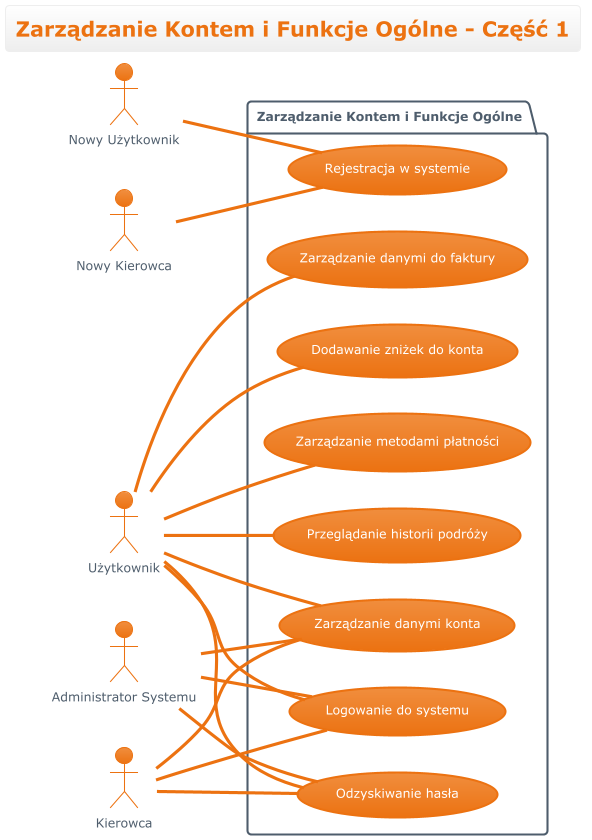
\includegraphics[width=0.8\linewidth]{diagramy/przypadki_uzycia/images/diagram_zarzadzanie_kontem_1.png}
    \caption{Diagram przypadków użycia: Funkcje ogólne - część 1}
    \label{fig:diag_zk_1}
\end{figure}
\begin{figure}[H]
    \centering
    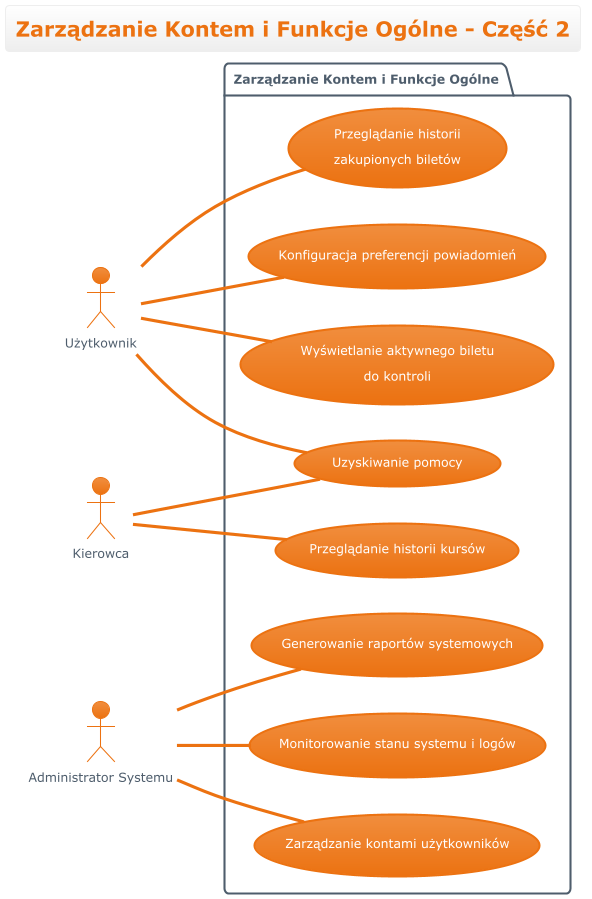
\includegraphics[width=0.8\linewidth]{diagramy/przypadki_uzycia/images/diagram_zarzadzanie_kontem_2.png}
    \caption{Diagram przypadków użycia: Funkcje ogólne - część 2}
    \label{fig:diag_zk_2}
\end{figure}
\begin{figure}[H]
    \centering
    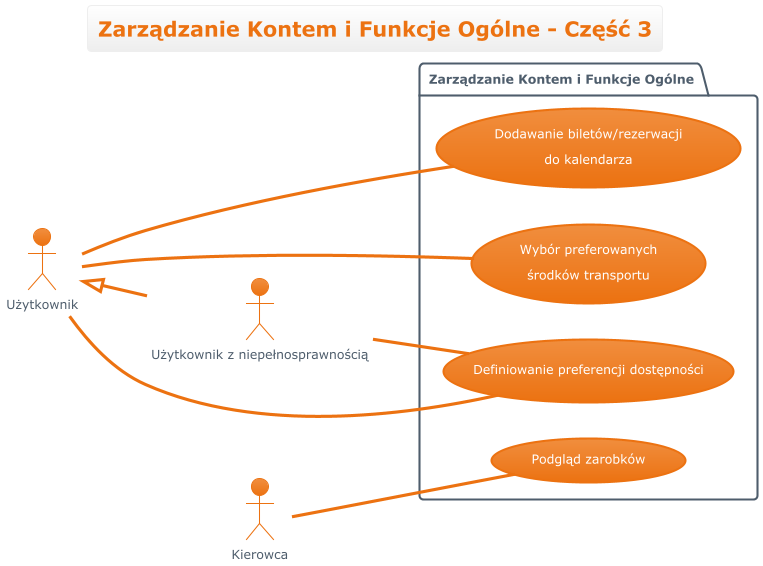
\includegraphics[width=0.8\linewidth]{diagramy/przypadki_uzycia/images/diagram_zarzadzanie_kontem_3.png}
    \caption{Diagram przypadków użycia: Funkcje ogólne - część 3}
    \label{fig:diag_zk_3}
\end{figure}

\subsubsection{Transport Publiczny}
\begin{enumerate}[label=\arabic*.]
    \item Wyszukiwanie połączeń komunikacji miejskiej (Użytkownik)
    \item Wyświetlanie rozkładu jazdy komunikacji miejskiej (Użytkownik)
    \item Zakup biletu jednorazowego na komunikację miejską (Użytkownik, Przewoźnik Miejski, Dostawca Usług Płatności)
    \item Zakup biletu okresowego na komunikację miejską (Użytkownik, Przewoźnik Miejski, Dostawca Usług Płatności)
    \item Planowanie trasy multimodalnej (Użytkownik)
    \item Zapisywanie ulubionych tras i przystanków (Użytkownik)
    \item Otrzymywanie powiadomień o zmianach w komunikacji miejskiej (Użytkownik)
    \item Dostarczanie danych o transporcie publicznym (Przewoźnik Miejski)
\end{enumerate}
\begin{figure}[H]
    \centering
    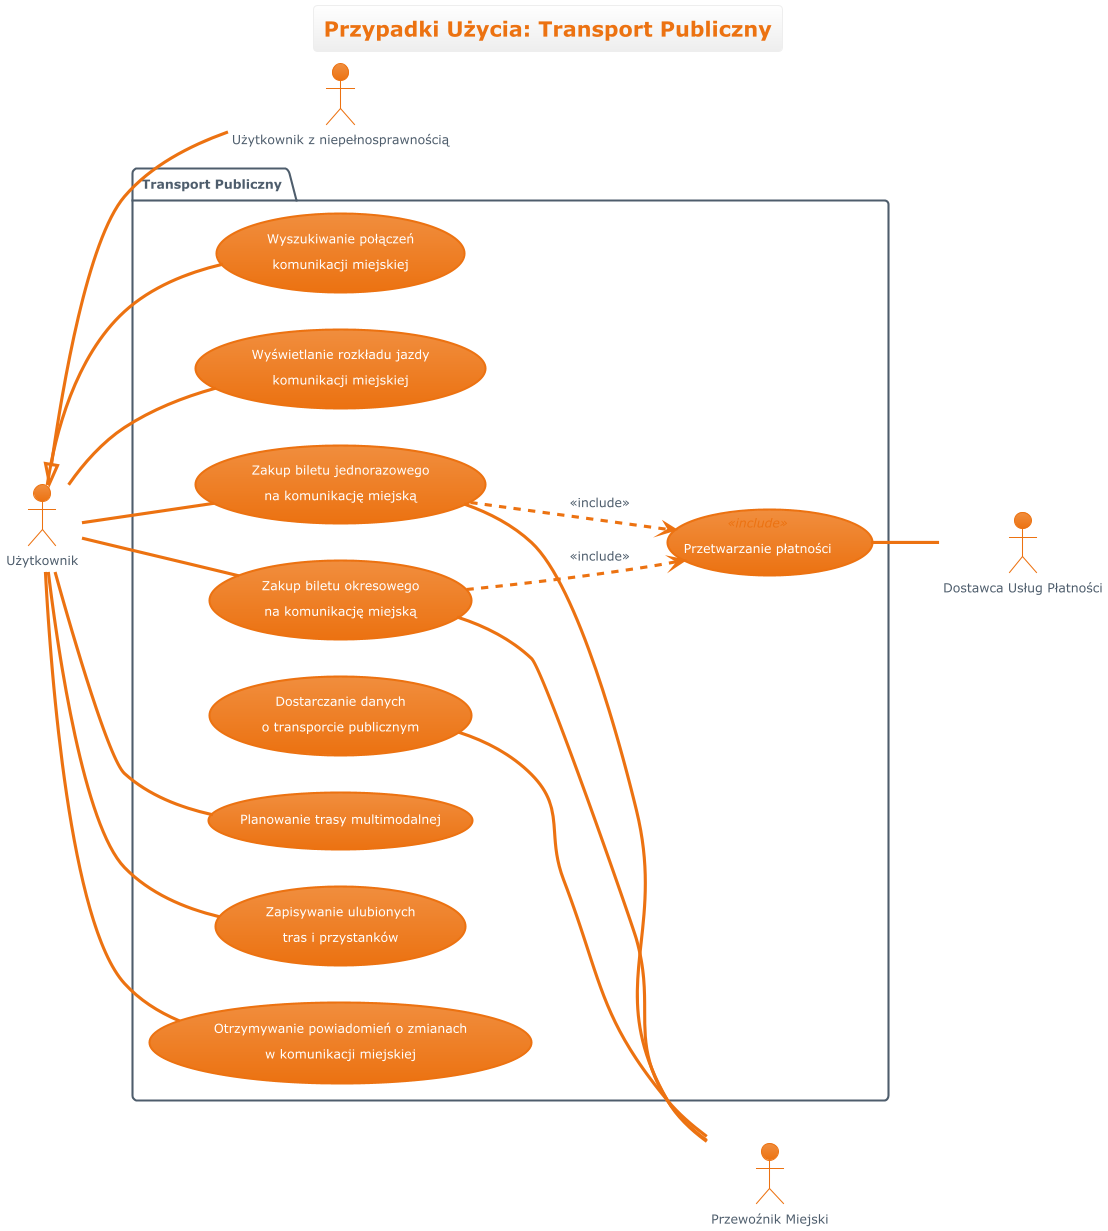
\includegraphics[width=0.9\linewidth]{diagramy/przypadki_uzycia/images/diagram_transport_publiczny.png}
    \caption{Diagram przypadków użycia: Transport publiczny}
    \label{fig:diag_tp}
\end{figure}

\subsubsection{Przejazdy Taksówką / Na Żądanie}
\begin{enumerate}[label=\arabic*.]
    \item Zamawianie przejazdu (Użytkownik, Przewoźnik Prywatny, Dostawca Usług Płatności)
    \item Rezerwacja przyszłego przejazdu (Użytkownik, Kierowca, Przewoźnik Prywatny, Dostawca Usług Płatności)
    \item Śledzenie lokalizacji zamówionego pojazdu (Użytkownik, Kierowca)
    \item Anulowanie zamówionego przejazdu (Użytkownik, Kierowca, Przewoźnik Prywatny, Dostawca Usług Płatności)
    \item Ocena kierowcy i przejazdu (Użytkownik)
    \item Otrzymywanie powiadomienia o przyjeździe pojazdu (Użytkownik)
    \item Akceptacja lub odrzucenie zlecenia (Kierowca, Przewoźnik Prywatny)
    \item Nawigowanie do miejsca odbioru pasażera (Kierowca)
    \item Zgłaszanie rozpoczęcia kursu (Kierowca)
    \item Zgłaszanie zakończenia kursu (Kierowca, Dostawca Usług Płatności)
    \item Zgłaszanie gotowości do przyjmowania zleceń (Kierowca)
\end{enumerate}
\begin{figure}[H]
    \centering
    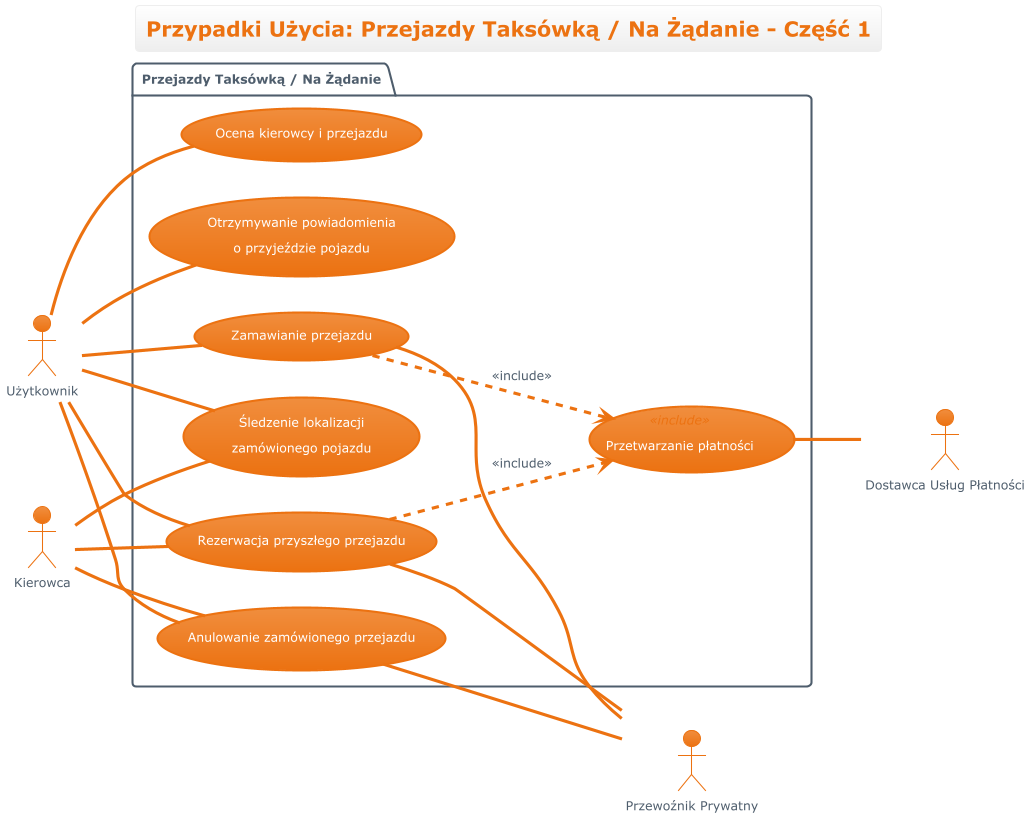
\includegraphics[width=0.8\linewidth]{diagramy/przypadki_uzycia/images/diagram_przejazdy_taksowka_1.png}
    \caption{Diagram przypadków użycia: Przejazdy taksówką / na żądanie - część 1}
    \label{fig:diag_pt_1}
\end{figure}
\begin{figure}[H]
    \centering
    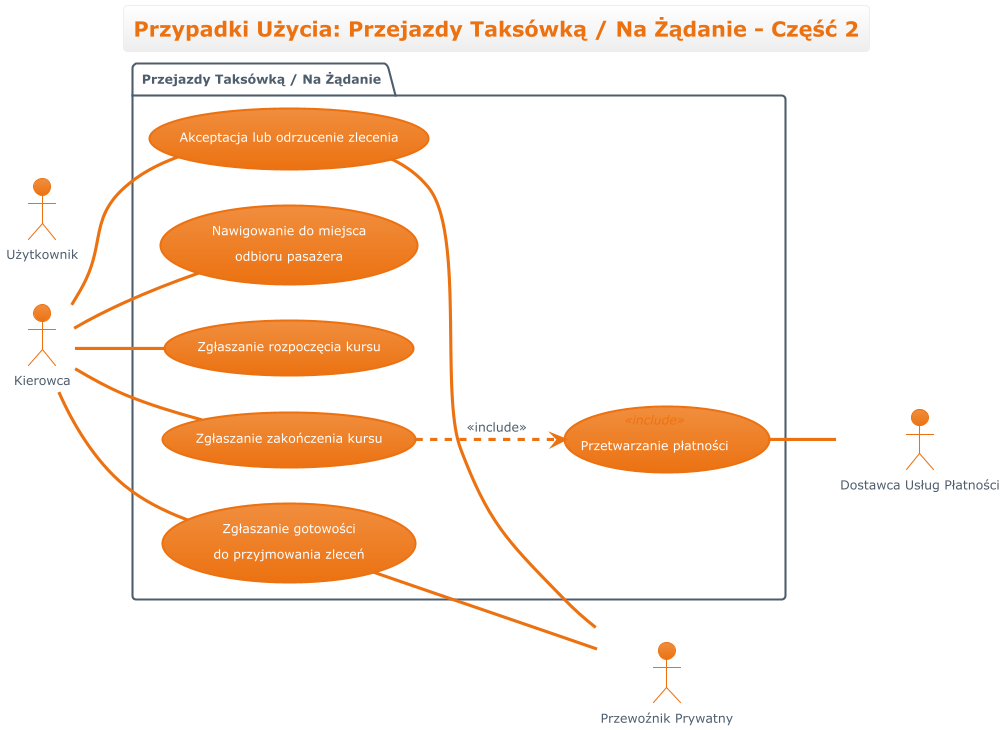
\includegraphics[width=0.8\linewidth]{diagramy/przypadki_uzycia/images/diagram_przejazdy_taksowka_2.png}
    \caption{Diagram przypadków użycia: Przejazdy taksówką / na żądanie - część 2}
    \label{fig:diag_pt_2}
\end{figure}

\subsubsection{Bilety Kolejowe}
\begin{enumerate}[label=\arabic*.]
    \item Wyszukiwanie połączeń kolejowych (Użytkownik)
    \item Wyświetlanie szczegółów połączenia kolejowego (Użytkownik)
    \item Wybór miejsca w pociągu (Użytkownik)
    \item Dodawanie danych pasażera (Użytkownik)
    \item Zakup biletu kolejowego (Użytkownik, Przewoźnik Kolejowy, Dostawca Usług Płatności)
    \item Otrzymywanie powiadomień o zmianach dotyczących podróży koleją (Użytkownik)
    \item Anulowanie biletu kolejowego (Użytkownik, Przewoźnik Kolejowy, Dostawca Usług Płatności)
    \item Wymiana biletu kolejowego (Użytkownik, Przewoźnik Kolejowy, Dostawca Usług Płatności)
    \item Pobieranie faktury za bilet kolejowy (Użytkownik)
\end{enumerate}
\begin{figure}[H]
    \centering
    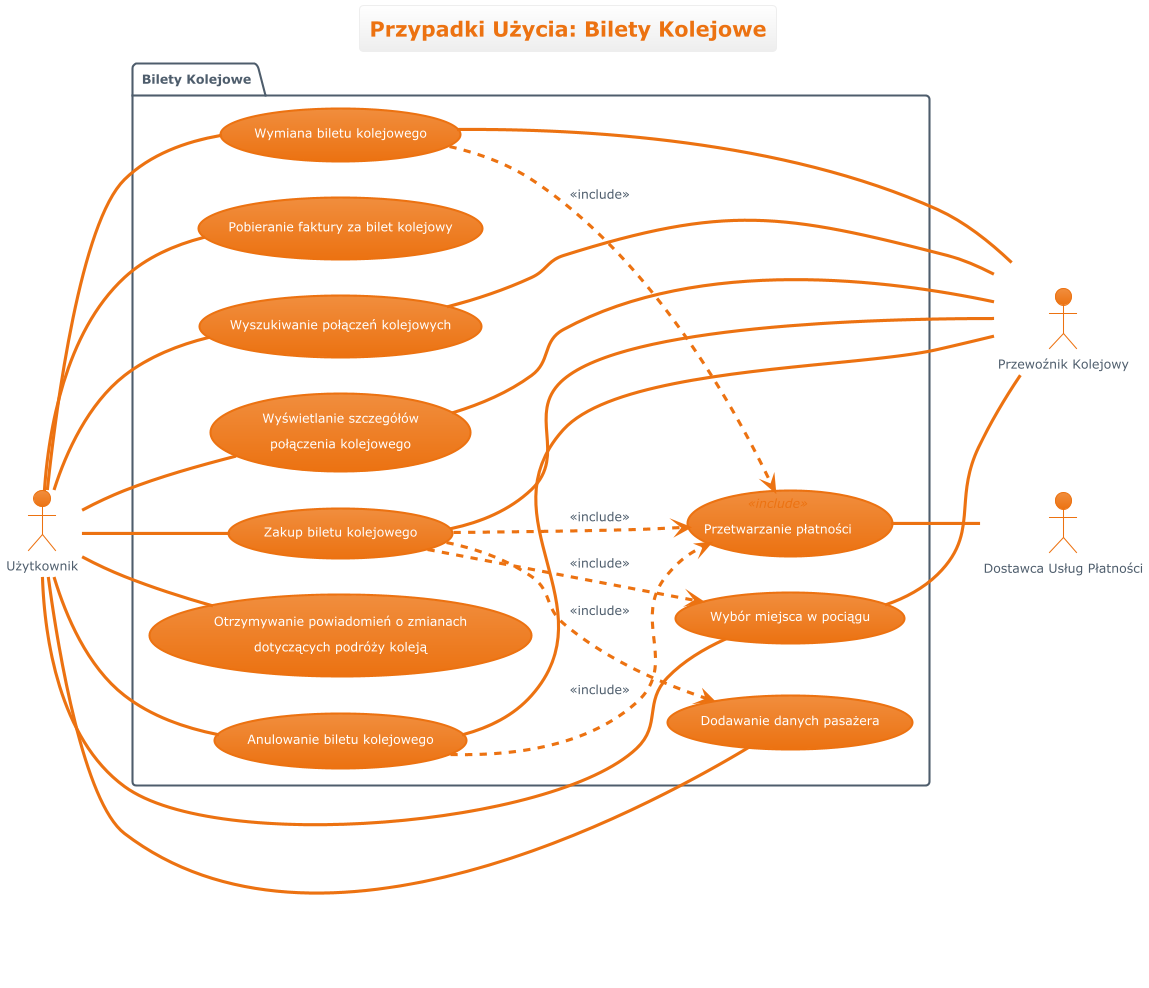
\includegraphics[width=0.8\linewidth]{diagramy/przypadki_uzycia/images/diagram_bilety_kolejowe_1.png}
    \caption{Diagram przypadków użycia: Bilety kolejowe}
    \label{fig:diag_bk_1}
\end{figure}

\subsubsection{Bilety Lotnicze}
\begin{enumerate}[label=\arabic*.]
    \item Ustawianie preferencji wyszukiwania lotów (Użytkownik)
    \item Zakup/Rezerwacja biletu lotniczego (Użytkownik, Przewoźnik lotniczy, Dostawca Usług Płatności)
    \item Wyszukiwanie połączeń lotniczych (Użytkownik)
    \item Wyświetlanie szczegółów połączenia lotniczego (Użytkownik)
    \item Porównywanie cen biletów lotniczych (Użytkownik)
    \item Dostarczanie danych o połączeniach i cenach biletów lotniczych (Przewoźnik Lotniczy)
    \item Rezerwacja transportu na/z lotniska (Użytkownik, Kierowca, Przewoźnik Prywatny, Dostawca Usług Płatności)
    \item Zarządzanie kartą pokładową (Użytkownik)
    \item Sprawdzanie statusu lotu (Użytkownik)
    \item Otrzymywanie alertów cenowych na loty (Użytkownik)
    \item Wyświetlanie mapy lotniska (Użytkownik)
\end{enumerate}
\begin{figure}[H]
    \centering
    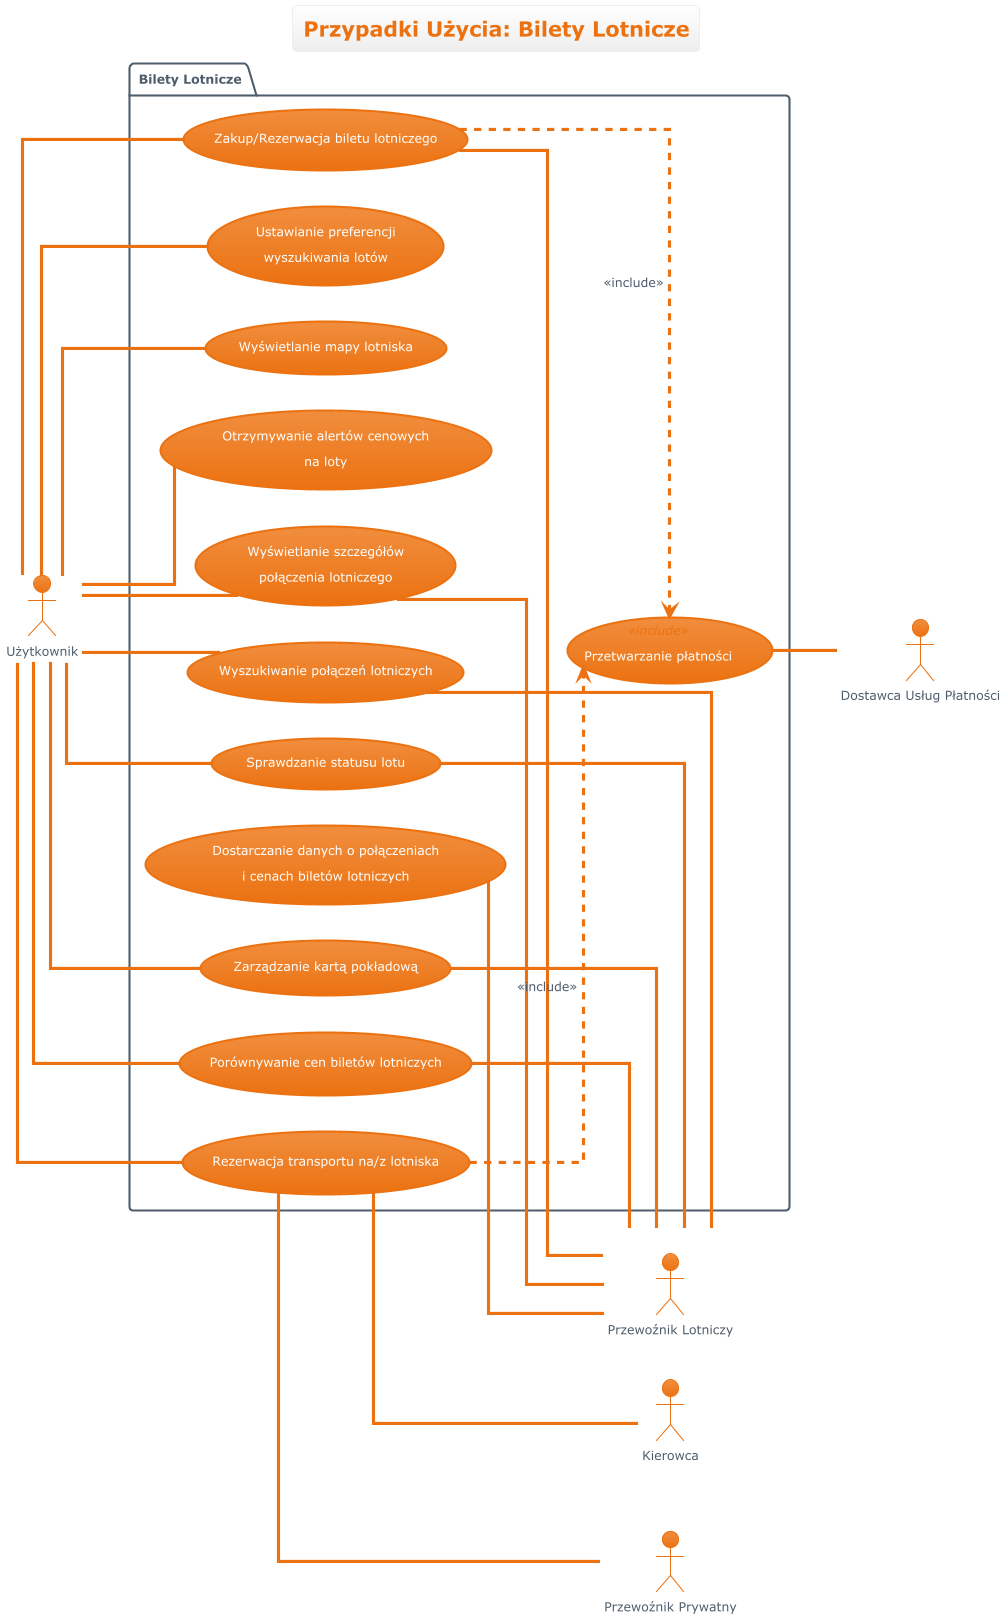
\includegraphics[width=0.8\linewidth]{diagramy/przypadki_uzycia/images/diagram_bilety_lotnicze_1.png}
    \caption{Diagram przypadków użycia: Bilety lotnicze}
    \label{fig:diag_bl_1}
\end{figure}

\newpage
\section{Scenariusze Przypadków Użycia}
\label{sec:scenarios}
Niniejszy rozdział zawiera szczegółowe scenariusze dla wybranych przypadków użycia zidentyfikowanych w systemie OpenTravel. Każdy scenariusz opisuje krok po kroku interakcję aktorów z systemem, warunki początkowe i końcowe, główny ciąg zdarzeń oraz możliwe alternatywne przebiegi i sytuacje wyjątkowe. Celem jest precyzyjne zdefiniowanie zachowania systemu w odpowiedzi na działania użytkowników i systemów zewnętrznych.

\subsection{Scenariusze dla modułu: Zarządzanie Kontem i Funkcje Ogólne}
W tej sekcji przedstawiono scenariusze przypadków użycia związane z podstawowymi funkcjami zarządzania kontem użytkownika, kierowcy oraz administratora, a także innymi ogólnymi operacjami dostępnymi w systemie OpenTravel. Obejmują one procesy takie jak rejestracja, logowanie, zarządzanie danymi osobowymi oraz inne funkcje wspólne dla różnych typów użytkowników.

\subsubsection{PU-ZK-01: Rejestracja w systemie}
\begin{itemize}
    \item \textbf{Nazwa przypadku użycia:} Rejestracja w systemie
    \item \textbf{Opis przypadku użycia:} Umożliwia nowym użytkownikom oraz kierowcom utworzenie konta w systemie OpenTravel poprzez podanie niezbędnych danych i ich weryfikację.
    \item \textbf{Aktorzy biorący udział:} Nowy Użytkownik, Nowy Kierowca
    \item \textbf{Uzasadnienie:} Zapewnienie nowym osobom możliwości dołączenia do platformy OpenTravel i korzystania z jej funkcjonalności.
    \item \textbf{Warunki początkowe:}
        \begin{itemize}
            \item Aktor (Nowy Użytkownik lub Nowy Kierowca) posiada dostęp do aplikacji mobilnej OpenTravel lub strony internetowej.
            \item Aktor nie jest zalogowany w systemie.
        \end{itemize}
    \item \textbf{Warunki końcowe:}
        \begin{itemize}
            \item Nowe konto Aktora zostało pomyślnie utworzone i zweryfikowane (jeśli wymagane).
            \item Dane nowego konta zostały zapisane w bazie danych systemu.
            \item Aktor jest gotowy do pierwszego logowania lub został automatycznie zalogowany.
        \end{itemize}
    \item \textbf{Główny ciąg zdarzeń:}
        \begin{enumerate}
            \item Aktor uruchamia aplikację mobilną OpenTravel lub otwiera stronę internetową.
            \item Aktor wybiera opcję "Zarejestruj się".
            \item System wyświetla formularz rejestracyjny zawierający następujące sekcje i pola: wybór typu konta (Użytkownik/Kierowca), dane logowania (adres e-mail, hasło, potwierdzenie hasła), dane osobowe (imię, nazwisko), numer telefonu, zgody (regulamin, polityka prywatności).
            \item Aktor wybiera typ konta (Użytkownik lub Kierowca – jeśli rozróżnienie jest na tym etapie).
            \item Aktor wypełnia wymagane pola formularza (adres e-mail, hasło, imię, nazwisko, numer telefonu). Konkretne pola mogą zależeć od typu konta.
            \item Aktor akceptuje regulamin systemu i politykę prywatności.
            \item Aktor wybiera przycisk potwierdzający chęć rejestracji (np. "Zarejestruj", "Utwórz konto").
            \item System przeprowadza walidację wprowadzonych danych (np. format adresu e-mail, siła hasła, kompletność danych).
            \item System wysyła wiadomość e-mail z linkiem aktywacyjnym na podany adres e-mail lub kod weryfikacyjny SMS na podany numer telefonu (w zależności od skonfigurowanej metody weryfikacji).
            \item Aktor odbiera wiadomość i klika w link aktywacyjny lub wprowadza otrzymany kod weryfikacyjny w odpowiednim polu w aplikacji/na stronie.
            \item System weryfikuje poprawność linku/kodu.
            \item System tworzy nowe konto w bazie danych, przypisując mu unikalny identyfikator oraz wybrany typ (Użytkownik/Kierowca).
            \item System oznacza konto jako aktywne/zweryfikowane.
            \item System wyświetla komunikat o pomyślnym zakończeniu rejestracji i może automatycznie zalogować Aktora lub przekierować go do ekranu logowania.
        \end{enumerate}
    \item \textbf{Alternatywne ciągi zdarzeń:}
        \begin{itemize}
            \item \textbf{A1: Rejestracja za pomocą konta zewnętrznego (np. Google, Facebook, Apple ID)}
                \begin{enumerate}
                    \item \textit{Kontekst: Zamiast/Po kroku 2 Głównego ciągu zdarzeń.} Aktor wybiera opcję rejestracji za pomocą jednego z dostępnych dostawców tożsamości (np. "Zarejestruj przez Google").
                    \item System inicjuje proces autoryzacji z wybranym dostawcą zewnętrznym (np. przekierowuje Aktora na stronę logowania dostawcy lub wyświetla systemowe okno dialogowe logowania).
                    \item Aktor loguje się na swoje konto u dostawcy zewnętrznego i udziela zgody na udostępnienie przez dostawcę określonych danych (np. adresu e-mail, imienia, nazwiska) systemowi OpenTravel.
                    \item System OpenTravel otrzymuje dane autoryzacyjne oraz profilowe od dostawcy zewnętrznego.
                    \item System tworzy nowe konto w bazie danych, wykorzystując otrzymane dane. Konto jest domyślnie oznaczane jako zweryfikowane.
                    \item System może poprosić Aktora o uzupełnienie dodatkowych informacji specyficznych dla OpenTravel, jeśli nie zostały one dostarczone przez zewnętrznego dostawcę (np. wybór typu konta Kierowca/Użytkownik, jeśli nie jest to domyślne).
                    \item System wyświetla komunikat o pomyślnym zakończeniu rejestracji i zazwyczaj automatycznie loguje Aktora. (Kontynuacja od kroku 14 Głównego ciągu zdarzeń).
                \end{enumerate}
        \end{itemize}
    \item \textbf{Sytuacje wyjątkowe:}
        \begin{itemize}
            \item \textbf{W1: Nieprawidłowe dane w formularzu.}
                \begin{enumerate}
                    \item \textit{Kontekst: Po kroku 8 Głównego ciągu zdarzeń.} System wykrywa błędy walidacji (np. niepoprawny format adresu e-mail, hasło nie spełnia wymagań bezpieczeństwa, brak wypełnienia obowiązkowych pól).
                    \item System wyświetla stosowne komunikaty o błędach przy odpowiednich polach formularza.
                    \item Aktor ma możliwość poprawienia danych. Scenariusz wraca do kroku 5 Głównego ciągu zdarzeń.
                \end{enumerate}
            \item \textbf{W2: Konto z podanym adresem e-mail lub numerem telefonu już istnieje.}
                \begin{enumerate}
                    \item \textit{Kontekst: Po kroku 8 Głównego ciągu zdarzeń.} System stwierdza, że podany unikalny identyfikator (np. adres e-mail) jest już zarejestrowany.
                    \item System wyświetla komunikat informujący, że konto już istnieje i sugeruje logowanie lub skorzystanie z opcji odzyskiwania hasła.
                    \item Proces rejestracji dla tych danych kończy się niepowodzeniem.
                \end{enumerate}
            \item \textbf{W3: Nieudana wysyłka wiadomości weryfikacyjnej.}
                \begin{enumerate}
                    \item \textit{Kontekst: Po kroku 9 Głównego ciągu zdarzeń.} System napotyka problem techniczny uniemożliwiający wysłanie wiadomości e-mail lub SMS.
                    \item System wyświetla komunikat o błędzie i może zaoferować opcję ponownego wysłania wiadomości lub kontakt z pomocą techniczną.
                \end{enumerate}
            \item \textbf{W4: Link aktywacyjny/kod weryfikacyjny jest nieprawidłowy lub wygasł.}
                \begin{enumerate}
                    \item \textit{Kontekst: Po kroku 11 Głównego ciągu zdarzeń.} System stwierdza, że użyty link aktywacyjny lub kod weryfikacyjny jest niepoprawny, został już użyty lub jego ważność wygasła.
                    \item System wyświetla komunikat o błędzie weryfikacji i może zaoferować opcję ponownego wysłania wiadomości weryfikacyjnej.
                \end{enumerate}
            \item \textbf{W5: Błąd autoryzacji przez dostawcę zewnętrznego (dotyczy A1).}
                \begin{enumerate}
                    \item \textit{Kontekst: Podczas kroku 3 Alternatywnego ciągu zdarzeń A1.} Dostawca zewnętrzny zwraca błąd autoryzacji lub Aktor nie udziela zgody.
                    \item System OpenTravel wyświetla komunikat o niepowodzeniu autoryzacji i sugeruje ponowienie próby lub wybór innej metody rejestracji.
                \end{enumerate}
        \end{itemize}
\end{itemize}

\subsection{Scenariusze dla modułu: Przejazdy Taksówką / Na Żądanie}
W tej sekcji przedstawiono szczegółowe scenariusze przypadków użycia związane z funkcjonalnościami zamawiania, realizacji i zarządzania przejazdami taksówkami lub innymi środkami transportu na żądanie w systemie OpenTravel. Obejmują one interakcje zarówno Użytkownika, jak i Kierowcy z platformą.

\subsubsection{PU-PT-01: Zamawianie przejazdu}
\begin{itemize}
    \item \textbf{Nazwa przypadku użycia:} Zamawianie przejazdu
    \item \textbf{Opis przypadku użycia:} Umożliwia Użytkownikowi zamówienie przejazdu "na teraz" (ASAP) poprzez określenie miejsca odbioru i docelowego, wybór typu pojazdu oraz potwierdzenie zamówienia i metody płatności.
    \item \textbf{Aktorzy biorący udział:} Użytkownik, Przewoźnik Prywatny (system zewnętrzny), Dostawca Usług Płatności (system zewnętrzny)
    \item \textbf{Uzasadnienie:} Zapewnienie Użytkownikowi możliwości szybkiego i wygodnego zamówienia dostępnego środka transportu w czasie rzeczywistym, bez konieczności ręcznego wyszukiwania czy dzwonienia.
    \item \textbf{Warunki początkowe:}
        \begin{itemize}
            \item Użytkownik jest zalogowany do aplikacji OpenTravel.
            \item Aplikacja ma dostęp do usług lokalizacyjnych urządzenia Użytkownika (lub Użytkownik ręcznie wprowadza adres odbioru).
            \item System ma aktywne połączenie z systemami Przewoźników Prywatnych.
            \item Użytkownik ma zdefiniowaną przynajmniej jedną metodę płatności w systemie lub jest gotowy ją dodać/wybrać.
        \end{itemize}
    \item \textbf{Warunki końcowe:}
        \begin{itemize}
            \item Zamówienie na przejazd zostało złożone i przyjęte przez system Przewoźnika Prywatnego.
            \item Najbliższy dostępny Kierowca (spełniający kryteria) został powiadomiony o zleceniu (lub zlecenie trafiło do puli oczekujących na akceptację).
            \item Użytkownik otrzymał potwierdzenie zamówienia wraz z szacowanym czasem oczekiwania na Kierowcę, przewidywaną ceną (lub zakresem cenowym) oraz danymi pojazdu i Kierowcy (jeśli już przydzielony).
            \item Płatność została wstępnie autoryzowana przez system Dostawcy Usług Płatności (jeśli dotyczy płatności bezgotówkowej).
        \end{itemize}
    \item \textbf{Główny ciąg zdarzeń:}
        \begin{enumerate}
            \item Użytkownik wybiera opcję "Zamów przejazd" lub "Taxi" w aplikacji OpenTravel.
            \item System automatycznie wykrywa aktualną lokalizację Użytkownika jako domyślne miejsce odbioru (z możliwością korekty przez Użytkownika na mapie lub przez wpisanie adresu).
            \item Użytkownik wprowadza adres docelowy (ręcznie, poprzez wyszukiwarkę adresów z autouzupełnianiem lub wskazanie na mapie).
            \item System wyświetla na mapie sugerowaną trasę przejazdu.
            \item System, na podstawie danych od zintegrowanych Przewoźników Prywatnych, prezentuje dostępne typy pojazdów/usług (np. Standard, Premium, XL, Eko, Dostosowany dla osób z niepełnosprawnościami) wraz z szacunkową ceną (lub widełkami cenowymi, informacją o mnożniku taryfy dynamicznej, jeśli ma zastosowanie) i przybliżonym czasem oczekiwania na przyjazd pojazdu dla każdego typu.
            \item Użytkownik wybiera preferowany typ pojazdu/usługi.
            \item System wyświetla podsumowanie zamówienia: miejsce odbioru, miejsce docelowe, wybrany typ pojazdu, szacowaną cenę/zakres cenowy, przewidywany czas oczekiwania oraz domyślną metodę płatności Użytkownika.
            \item Użytkownik ma możliwość zmiany metody płatności (jeśli ma ich kilka lub chce dodać nową, np. płatność gotówką, o ile jest akceptowana przez Przewoźnika).
            \item Użytkownik potwierdza zamówienie przejazdu (np. przyciskiem "Zamów teraz" lub "Potwierdź").
            \item Jeśli wybrano płatność bezgotówkową, system OpenTravel inicjuje wstępną autoryzację szacowanej kwoty u Dostawcy Usług Płatności.
            \item System OpenTravel wysyła zlecenie (zawierające szczegóły przejazdu i Użytkownika) do systemu odpowiedniego Przewoźnika Prywatnego.
            \item System Przewoźnika Prywatnego wyszukuje najbliższego dostępnego Kierowcę spełniającego kryteria (typ pojazdu, lokalizacja) i przydziela mu zlecenie lub umieszcza zlecenie w puli dostępnej dla Kierowców.
            \item System Przewoźnika Prywatnego zwraca do OpenTravel potwierdzenie przyjęcia zamówienia oraz, gdy Kierowca zostanie przydzielony, jego dane (imię, zdjęcie, ocena, marka i numer rejestracyjny pojazdu) oraz zaktualizowany czas przyjazdu.
            \item System OpenTravel wyświetla Użytkownikowi potwierdzenie zamówienia, szacowany czas przyjazdu Kierowcy, jego dane oraz umożliwia śledzenie pojazdu na mapie (przejście do PU-PT-03).
        \end{enumerate}
    \item \textbf{Alternatywne ciągi zdarzeń:}
        \begin{itemize}
            \item \textbf{A1: Brak dostępnych pojazdów wybranego typu.}
                \begin{enumerate}
                    \item \textit{Kontekst: Po kroku 6 Głównego ciągu zdarzeń.} System informuje Użytkownika o braku dostępnych pojazdów wybranego typu w najbliższej okolicy lub o długim czasie oczekiwania.
                    \item System może zasugerować wybór innego typu pojazdu, zmianę miejsca odbioru lub spróbowanie później.
                \end{enumerate}
            \item \textbf{A2: Użytkownik dodaje notatkę dla Kierowcy.}
                \begin{enumerate}
                    \item \textit{Kontekst: Przed krokiem 9 Głównego ciągu zdarzeń.} Użytkownik ma możliwość dodania krótkiej notatki dla Kierowcy (np. "Proszę czekać przy bramie nr 5", "Mam duży bagaż").
                    \item Notatka jest przekazywana Kierowcy wraz ze zleceniem.
                \end{enumerate}
             \item \textbf{A3: Płatność gotówką.}
                \begin{enumerate}
                    \item \textit{Kontekst: Krok 8 Głównego ciągu zdarzeń.} Użytkownik wybiera płatność gotówką (jeśli opcja jest dostępna dla danego Przewoźnika/Kierowcy).
                    \item Krok 10 (wstępna autoryzacja) jest pomijany. System informuje Przewoźnika o wybranej formie płatności.
                \end{enumerate}
        \end{itemize}
    \item \textbf{Sytuacje wyjątkowe:}
        \begin{itemize}
            \item \textbf{W1: Problem z usługami lokalizacyjnymi.}
                \begin{enumerate}
                    \item \textit{Kontekst: Krok 2 Głównego ciągu zdarzeń.} System nie może uzyskać dostępu do lokalizacji Użytkownika (np. wyłączone usługi GPS, brak uprawnień aplikacji).
                    \item System prosi Użytkownika o ręczne wprowadzenie adresu odbioru lub włączenie usług lokalizacyjnych.
                \end{enumerate}
            \item \textbf{W2: Brak dostępnych jakichkolwiek pojazdów w okolicy.}
                \begin{enumerate}
                    \item \textit{Kontekst: Po kroku 5 Głównego ciągu zdarzeń.} System nie znajduje żadnych dostępnych Kierowców/pojazdów w akceptowalnym promieniu od miejsca odbioru.
                    \item System wyświetla komunikat: "Brak dostępnych pojazdów w Twojej okolicy. Spróbuj ponownie później."
                \end{enumerate}
            \item \textbf{W3: Nieudana wstępna autoryzacja płatności.}
                \begin{enumerate}
                    \item \textit{Kontekst: Po kroku 10 Głównego ciągu zdarzeń.} Dostawca Usług Płatności odrzuca próbę autoryzacji (np. niewystarczające środki, błędne dane karty, blokada karty).
                    \item System OpenTravel informuje Użytkownika o problemie z płatnością i prosi o wybór innej metody płatności lub aktualizację danych obecnej. Zamówienie nie jest wysyłane do Przewoźnika do czasu rozwiązania problemu z płatnością. Scenariusz wraca do kroku 8.
                \end{enumerate}
            \item \textbf{W4: Błąd komunikacji z systemem Przewoźnika Prywatnego lub Dostawcy Usług Płatności.}
                \begin{enumerate}
                    \item \textit{Kontekst: Podczas kroków 5, 10, 11 lub 13 Głównego ciągu zdarzeń.} System OpenTravel napotyka problem z komunikacją.
                    \item System wyświetla komunikat o błędzie technicznym i może zasugerować ponowienie próby. Jeśli błąd wystąpił po autoryzacji płatności, a przed potwierdzeniem przez Przewoźnika, autoryzacja powinna zostać anulowana.
                \end{enumerate}
            \item \textbf{W5: Zbyt wysoki mnożnik taryfy dynamicznej (surge pricing).}
                 \begin{enumerate}
                    \item \textit{Kontekst: Krok 5 Głównego ciągu zdarzeń.} System wyświetla informację o znacznie podwyższonej cenie z powodu dużego popytu.
                    \item System wyświetla wyraźne ostrzeżenie o wysokim mnożniku i ostatecznej szacowanej cenie.
                    \item Użytkownik może zaakceptować wyższą cenę i kontynuować zamówienie lub zrezygnować i spróbować później.
                \end{enumerate}
        \end{itemize}
\end{itemize}

\subsubsection{PU-PT-02: Rezerwacja przyszłego przejazdu}
\begin{itemize}
    \item \textbf{Nazwa przypadku użycia:} Rezerwacja przyszłego przejazdu
    \item \textbf{Opis przypadku użycia:} Umożliwia Użytkownikowi zarezerwowanie przejazdu na określoną datę i godzinę w przyszłości.
    \item \textbf{Aktorzy biorący udział:} Użytkownik, Kierowca (potencjalnie, jeśli system pozwala na wcześniejsze przypisanie), Przewoźnik Prywatny (system zewnętrzny), Dostawca Usług Płatności (system zewnętrzny)
    \item \textbf{Uzasadnienie:} Zapewnienie Użytkownikowi możliwości zaplanowania transportu z wyprzedzeniem, np. na lotnisko, ważne spotkanie.
    \item \textbf{Warunki początkowe:}
        \begin{itemize}
            \item Użytkownik jest zalogowany do aplikacji OpenTravel.
            \item System Przewoźnika Prywatnego wspiera funkcję rezerwacji terminowych.
            \item Użytkownik ma zdefiniowaną metodę płatności.
        \end{itemize}
    \item \textbf{Warunki końcowe:}
        \begin{itemize}
            \item Rezerwacja na przyszły przejazd została złożona i potwierdzona przez system Przewoźnika Prywatnego.
            \item Użytkownik otrzymał potwierdzenie rezerwacji z jej szczegółami (data, godzina, trasa, szacowana cena).
            \item Płatność może być autoryzowana lub pobrana z góry, w zależności od polityki Przewoźnika.
            \item System przypomni Użytkownikowi o zbliżającej się rezerwacji.
        \end{itemize}
    \item \textbf{Główny ciąg zdarzeń:}
        \begin{enumerate}
            \item Użytkownik wybiera opcję "Zaplanuj przejazd" lub "Rezerwacja terminowa" w sekcji zamawiania taksówki.
            \item System wyświetla formularz zamówienia, prosząc o podanie:
                \begin{itemize}
                    \item Adresu odbioru (wpisanie ręczne, wybór z mapy lub z zapisanych adresów).
                    \item Adresu docelowego (wpisanie ręczne, wybór z mapy lub z zapisanych adresów).
                    \item Daty i godziny odbioru (wybór z kalendarza i zegara, z uwzględnieniem minimalnego czasu wyprzedzenia wymaganego przez Przewoźnika).
                    \item Opcjonalnie: liczby pasażerów, ilości bagażu.
                \end{itemize}
            \item Użytkownik wypełnia wszystkie wymagane pola.
            \item System, na podstawie wprowadzonych danych, kontaktuje się z systemami Przewoźników Prywatnych w celu sprawdzenia dostępności usługi rezerwacji terminowej i uzyskania szacunkowej ceny dla różnych typów pojazdów.
            \item System wyświetla dostępne typy pojazdów/usług wraz z szacowaną ceną.
            \item Użytkownik wybiera preferowany typ pojazdu/usługi.
            \item System wyświetla podsumowanie rezerwacji: miejsce odbioru, miejsce docelowe, data i godzina, wybrany typ pojazdu, szacowana cena, wybrana metoda płatności.
            \item Użytkownik potwierdza rezerwację (np. przyciskiem "Zarezerwuj").
            \item System OpenTravel wysyła zlecenie rezerwacji do systemu odpowiedniego Przewoźnika Prywatnego.
            \item System Przewoźnika Prywatnego potwierdza przyjęcie rezerwacji. Może nastąpić wstępna autoryzacja płatności u Dostawcy Usług Płatności.
            \item System OpenTravel wyświetla Użytkownikowi potwierdzenie rezerwacji i zapisuje ją w historii zamówień.
            \item Na określony czas przed terminem odbioru (np. 30 minut), system Przewoźnika Prywatnego przypisuje konkretnego Kierowcę i pojazd do zlecenia. Informacje te są przekazywane do OpenTravel.
            \item System OpenTravel wysyła Użytkownikowi powiadomienie przypominające o zbliżającej się rezerwacji, zawierające dane przydzielonego Kierowcy i pojazdu.
        \end{enumerate}
    \item \textbf{Alternatywne ciągi zdarzeń:}
        \begin{itemize}
            \item \textbf{A1: Zmiana lub anulowanie rezerwacji terminowej.}
                \begin{enumerate}
                    \item Użytkownik, przed upływem określonego terminu, może zmodyfikować szczegóły rezerwacji (np. godzinę, adres) lub ją anulować (może się to wiązać z opłatą zgodnie z regulaminem Przewoźnika - patrz PU-PT-04).
                \end{enumerate}
        \end{itemize}
    \item \textbf{Sytuacje wyjątkowe:}
        \begin{itemize}
            \item \textbf{W1: Brak możliwości rezerwacji terminowej dla podanych kryteriów.}
                \begin{enumerate}
                    \item \textit{Kontekst: Po kroku 4 Głównego ciągu zdarzeń.} System Przewoźnika Prywatnego informuje, że rezerwacja terminowa dla podanej daty/godziny/lokalizacji nie jest możliwa (np. zbyt krótki czas wyprzedzenia, brak dostępnych pojazdów w systemie przewoźnika na ten termin).
                    \item System wyświetla stosowny komunikat. Użytkownik może zmienić parametry rezerwacji.
                \end{enumerate}
            \item \textbf{W2: Problem z potwierdzeniem rezerwacji przez system Przewoźnika Prywatnego.}
                \begin{enumerate}
                    \item \textit{Kontekst: Po kroku 9 Głównego ciągu zdarzeń.} System Przewoźnika nie może potwierdzić rezerwacji z powodu błędu technicznego.
                    \item System OpenTravel informuje Użytkownika o problemie i ewentualnie anuluje wstępną autoryzację płatności.
                \end{enumerate}
            \item \textbf{W3: Brak dostępnego kierowcy przed terminem realizacji zlecenia.}
                \begin{enumerate}
                     \item \textit{Kontekst: Krok 12 Głównego ciągu zdarzeń.} Pomimo wcześniejszej rezerwacji, system Przewoźnika Prywatnego nie może znaleźć dostępnego Kierowcy na krótko przed planowanym odbiorem.
                     \item System Przewoźnika Prywatnego informuje o tym system OpenTravel.
                     \item System OpenTravel natychmiast powiadamia Użytkownika o problemie z realizacją rezerwacji i proponuje alternatywne rozwiązania (np. próba zamówienia przejazdu "na teraz", kontakt z obsługą klienta Przewoźnika). Ewentualna przedpłata jest zwracana.
                 \end{enumerate}
        \end{itemize}
\end{itemize}

\subsubsection{PU-PT-03: Śledzenie lokalizacji zamówionego pojazdu}
\begin{itemize}
    \item \textbf{Nazwa przypadku użycia:} Śledzenie lokalizacji zamówionego pojazdu
    \item \textbf{Opis przypadku użycia:} Umożliwia Użytkownikowi śledzenie na mapie w czasie rzeczywistym lokalizacji Kierowcy zmierzającego do miejsca odbioru. Kierowca również może widzieć przybliżoną lokalizację Użytkownika (jeśli Użytkownik udostępnia lokalizację).
    \item \textbf{Aktorzy biorący udział:} Użytkownik, Kierowca
    \item \textbf{Uzasadnienie:} Zwiększenie komfortu i poczucia bezpieczeństwa Użytkownika poprzez dostarczanie aktualnych informacji o położeniu zamówionego pojazdu i przewidywanym czasie jego przybycia. Ułatwia Kierowcy dotarcie do Użytkownika.
    \item \textbf{Warunki początkowe:}
        \begin{itemize}
            \item Użytkownik pomyślnie zamówił przejazd (zakończony PU-PT-01 lub aktywna rezerwacja terminowa PU-PT-02, do której został już przydzielony Kierowca).
            \item Kierowca zaakceptował zlecenie i jest w drodze do miejsca odbioru Użytkownika.
            \item Zarówno urządzenie Użytkownika, jak i Kierowcy mają włączone usługi lokalizacyjne i dostęp do sieci.
        \end{itemize}
    \item \textbf{Warunki końcowe:}
        \begin{itemize}
            \item Użytkownik widzi na mapie w aplikacji OpenTravel ikonę reprezentującą pojazd Kierowcy oraz jego aktualne położenie.
            \item Kierowca widzi na mapie w swojej aplikacji lokalizację miejsca odbioru i ewentualnie przybliżoną, anonimizowaną lokalizację Użytkownika.
            \item Informacje o lokalizacji są aktualizowane w czasie rzeczywistym.
        \end{itemize}
    \item \textbf{Główny ciąg zdarzeń:}
        \begin{enumerate}
            \item Po przydzieleniu Kierowcy do zamówienia Użytkownika, aplikacja OpenTravel (Użytkownika) automatycznie wyświetla mapę z zaznaczonym miejscem odbioru i ikoną pojazdu Kierowcy.
            \item Aplikacja Kierowcy regularnie wysyła dane o jego aktualnej lokalizacji GPS do systemu Przewoźnika Prywatnego.
            \item System Przewoźnika Prywatnego przekazuje te dane (lub przetworzone) do systemu OpenTravel.
            \item System OpenTravel aktualizuje położenie ikony pojazdu Kierowcy na mapie Użytkownika.
            \item Aplikacja OpenTravel (Użytkownika) może również wysyłać (za zgodą Użytkownika) jego przybliżoną, anonimizowaną lokalizację do systemu, aby ułatwić Kierowcy odnalezienie, szczególnie jeśli Użytkownik przemieszcza się w obrębie miejsca odbioru.
            \item Aplikacja Użytkownika wyświetla również zaktualizowany szacowany czas przyjazdu Kierowcy (ETA).
            \item Proces śledzenia trwa aż do momentu, gdy Kierowca zgłosi przybycie na miejsce odbioru.
        \end{enumerate}
    \item \textbf{Alternatywne ciągi zdarzeń:}
        \begin{itemize}
            \item \textbf{A1: Użytkownik wyłącza udostępnianie swojej lokalizacji Kierowcy.}
                \begin{enumerate}
                    \item Użytkownik w ustawieniach aplikacji może zrezygnować z udostępniania swojej lokalizacji Kierowcy. Kierowca będzie widział jedynie ustalony punkt odbioru.
                \end{enumerate}
        \end{itemize}
    \item \textbf{Sytuacje wyjątkowe:}
        \begin{itemize}
            \item \textbf{W1: Utrata połączenia GPS lub sieciowego przez Kierowcę.}
                \begin{enumerate}
                    \item Aplikacja Kierowcy traci możliwość wysyłania aktualizacji lokalizacji.
                    \item Aplikacja Użytkownika wyświetla ostatnią znaną lokalizację Kierowcy z informacją o możliwym opóźnieniu w aktualizacji lub komunikatem "Problem z lokalizacją kierowcy".
                    \item System próbuje przywrócić połączenie.
                \end{enumerate}
            \item \textbf{W2: Utrata połączenia sieciowego przez Użytkownika.}
                \begin{enumerate}
                    \item Aplikacja Użytkownika nie może odbierać aktualizacji lokalizacji Kierowcy.
                    \item Aplikacja wyświetla stosowny komunikat o problemie z połączeniem sieciowym.
                \end{enumerate}
        \end{itemize}
\end{itemize}

\subsubsection{PU-PT-04: Anulowanie zamówionego przejazdu}
\begin{itemize}
    \item \textbf{Nazwa przypadku użycia:} Anulowanie zamówionego przejazdu
    \item \textbf{Opis przypadku użycia:} Umożliwia Użytkownikowi lub Kierowcy anulowanie przyjętego zlecenia na przejazd, zgodnie z regulaminem Przewoźnika (może wiązać się z opłatą za anulowanie po określonym czasie).
    \item \textbf{Aktorzy biorący udział:} Użytkownik, Kierowca, Przewoźnik Prywatny (system zewnętrzny), Dostawca Usług Płatności (system zewnętrzny - dla ewentualnej opłaty za anulowanie)
    \item \textbf{Uzasadnienie:} Zapewnienie elastyczności w przypadku zmiany planów lub nieprzewidzianych okoliczności zarówno dla Użytkownika, jak i Kierowcy.
    \item \textbf{Warunki początkowe:}
        \begin{itemize}
            \item Przejazd został zamówiony (zakończony PU-PT-01 lub aktywna rezerwacja PU-PT-02) i Kierowca został przydzielony (lub zlecenie jest w puli).
            \item Kurs się jeszcze nie rozpoczął.
        \end{itemize}
    \item \textbf{Warunki końcowe:}
        \begin{itemize}
            \item Zamówienie przejazdu zostało anulowane w systemie OpenTravel oraz w systemie Przewoźnika Prywatnego.
            \item Druga strona (Kierowca lub Użytkownik) została powiadomiona o anulowaniu.
            \item Ewentualna opłata za anulowanie została naliczona i pobrana od Użytkownika (jeśli dotyczy).
            \item Kierowca (jeśli był już w drodze) może otrzymać rekompensatę (zależnie od polityki Przewoźnika).
        \end{itemize}
    \item \textbf{Główny ciąg zdarzeń (Anulowanie przez Użytkownika):}
        \begin{enumerate}
            \item Użytkownik wybiera opcję "Anuluj przejazd" w szczegółach aktywnego zamówienia.
            \item System wyświetla informację o ewentualnej opłacie za anulowanie, jeśli ma zastosowanie (np. jeśli Kierowca jest już w drodze lub minął określony czas od zamówienia).
            \item Użytkownik potwierdza chęć anulowania.
            \item System OpenTravel wysyła żądanie anulowania do systemu Przewoźnika Prywatnego.
            \item System Przewoźnika Prywatnego przetwarza anulowanie, powiadamia Kierowcę (jeśli był przydzielony) i potwierdza anulowanie do OpenTravel.
            \item Jeśli naliczono opłatę za anulowanie, system OpenTravel inicjuje jej pobranie za pośrednictwem Dostawcy Usług Płatności z domyślnej metody płatności Użytkownika.
            \item System OpenTravel wyświetla Użytkownikowi potwierdzenie anulowania oraz informację o ewentualnie pobranej opłacie.
        \end{enumerate}
    \item \textbf{Główny ciąg zdarzeń (Anulowanie przez Kierowcę):}
        \begin{enumerate}
            \item Kierowca, z ważnego powodu (np. awaria pojazdu, nieprzewidziane zdarzenie), wybiera opcję anulowania przyjętego zlecenia w swojej aplikacji.
            \item Aplikacja Kierowcy może wymagać podania przyczyny anulowania.
            \item Żądanie anulowania jest wysyłane do systemu Przewoźnika Prywatnego.
            \item System Przewoźnika Prywatnego przetwarza anulowanie i powiadamia system OpenTravel.
            \item System OpenTravel natychmiast informuje Użytkownika o anulowaniu przejazdu przez Kierowcę.
            \item System OpenTravel (lub Przewoźnika Prywatnego) może automatycznie rozpocząć wyszukiwanie innego, najbliższego Kierowcy dla Użytkownika lub zaproponować Użytkownikowi ponowne złożenie zamówienia.
        \end{enumerate}
    \item \textbf{Alternatywne ciągi zdarzeń:}
        \begin{itemize}
            \item \textbf{A1: Anulowanie bez opłaty.}
                \begin{enumerate}
                    \item \textit{Kontekst: Krok 2 Głównego ciągu zdarzeń (Anulowanie przez Użytkownika).} Użytkownik anuluje przejazd w okresie, w którym nie jest naliczana opłata (np. krótko po zamówieniu, zanim Kierowca zostanie przydzielony lub wyruszy).
                    \item Krok 6 (pobranie opłaty) jest pomijany.
                \end{enumerate}
        \end{itemize}
    \item \textbf{Sytuacje wyjątkowe:}
        \begin{itemize}
            \item \textbf{W1: Próba anulowania po rozpoczęciu kursu.}
                \begin{enumerate}
                    \item Użytkownik lub Kierowca próbuje anulować przejazd po tym, jak Kierowca zgłosił jego rozpoczęcie.
                    \item System odrzuca próbę anulowania, informując, że kurs już trwa.
                \end{enumerate}
            \item \textbf{W2: Problem z pobraniem opłaty za anulowanie.}
                \begin{enumerate}
                    \item \textit{Kontekst: Po kroku 6 Głównego ciągu zdarzeń (Anulowanie przez Użytkownika).} Dostawca Usług Płatności odrzuca transakcję pobrania opłaty.
                    \item System OpenTravel informuje Użytkownika o problemie. Niezapłacona opłata może zostać dodana do kolejnego zamówienia lub konto Użytkownika może zostać tymczasowo zablokowane do czasu uregulowania należności.
                \end{enumerate}
            \item \textbf{W3: Błąd komunikacji podczas procesu anulowania.}
                \begin{enumerate}
                    \item System napotyka problem z komunikacją z systemem Przewoźnika Prywatnego lub Dostawcy Usług Płatności.
                    \item System wyświetla komunikat o błędzie i sugeruje ponowienie próby lub kontakt z obsługą. Status anulowania może być niejasny do czasu rozwiązania problemu.
                \end{enumerate}
        \end{itemize}
\end{itemize}

\subsubsection{PU-PT-05: Ocena kierowcy i przejazdu}
\begin{itemize}
    \item \textbf{Nazwa przypadku użycia:} Ocena kierowcy i przejazdu
    \item \textbf{Opis przypadku użycia:} Umożliwia Użytkownikowi wystawienie oceny (np. w skali gwiazdek) oraz opcjonalnie komentarza na temat zakończonego przejazdu i obsługi przez Kierowcę.
    \item \textbf{Aktorzy biorący udział:} Użytkownik
    \item \textbf{Uzasadnienie:} Zbieranie informacji zwrotnych na temat jakości usług świadczonych przez Kierowców, co pomaga w utrzymaniu standardów, a także dostarcza innym Użytkownikom informacji przy wyborze usług.
    \item \textbf{Warunki początkowe:}
        \begin{itemize}
            \item Użytkownik zrealizował przejazd zamówiony przez aplikację OpenTravel.
            \item Kierowca zgłosił zakończenie kursu (zakończony PU-PT-10).
            \item Płatność za kurs została przetworzona.
        \end{itemize}
    \item \textbf{Warunki końcowe:}
        \begin{itemize}
            \item Ocena i ewentualny komentarz Użytkownika dotyczące przejazdu i Kierowcy zostały zapisane w systemie.
            \item Ocena może wpłynąć na ogólną ocenę Kierowcy widoczną dla innych Użytkowników i Przewoźnika Prywatnego.
        \end{itemize}
    \item \textbf{Główny ciąg zdarzeń:}
        \begin{enumerate}
            \item Po zakończeniu kursu i przetworzeniu płatności, aplikacja OpenTravel wyświetla Użytkownikowi ekran z prośbą o ocenę przejazdu i Kierowcy.
            \item System prezentuje skalę ocen (np. od 1 do 5 gwiazdek) oraz opcjonalne pole tekstowe na komentarz.
            \item Użytkownik wybiera ocenę gwiazdkową.
            \item Użytkownik opcjonalnie wprowadza komentarz dotyczący przejazdu (np. czystość pojazdu, uprzejmość Kierowcy, styl jazdy).
            \item Użytkownik może mieć możliwość wyboru predefiniowanych tagów opisujących pozytywne lub negatywne aspekty przejazdu.
            \item Użytkownik zatwierdza ocenę (np. przyciskiem "Wyślij ocenę").
            \item System OpenTravel zapisuje ocenę i komentarz, powiązując je z danym przejazdem i profilem Kierowcy.
            \item System wyświetla Użytkownikowi podziękowanie za wystawienie oceny.
        \end{enumerate}
    \item \textbf{Alternatywne ciągi zdarzeń:}
        \begin{itemize}
            \item \textbf{A1: Użytkownik pomija wystawienie oceny.}
                \begin{enumerate}
                    \item Użytkownik może zamknąć ekran oceny bez jej wystawiania.
                    \item System może przypomnieć o możliwości oceny później (np. w historii przejazdów) przez określony czas.
                \end{enumerate}
            \item \textbf{A2: Zgłoszenie problemu z przejazdem.}
                 \begin{enumerate}
                    \item Oprócz oceny, Użytkownik ma możliwość zgłoszenia poważniejszego problemu z przejazdem (np. niebezpieczne zachowanie Kierowcy, zagubiony przedmiot) poprzez dedykowaną opcję, która może uruchomić osobny proces kontaktu z obsługą klienta.
                \end{enumerate}
        \end{itemize}
    \item \textbf{Sytuacje wyjątkowe:}
        \begin{itemize}
            \item \textbf{W1: Błąd zapisu oceny.}
                \begin{enumerate}
                    \item System napotyka problem techniczny podczas próby zapisania oceny.
                    \item System wyświetla komunikat o błędzie i może umożliwić ponowną próbę zapisu.
                \end{enumerate}
        \end{itemize}
\end{itemize}

\subsubsection{PU-PT-06: Otrzymywanie powiadomienia o przyjeździe pojazdu}
\begin{itemize}
    \item \textbf{Nazwa przypadku użycia:} Otrzymywanie powiadomienia o przyjeździe pojazdu
    \item \textbf{Opis przypadku użycia:} Użytkownik otrzymuje automatyczne powiadomienie (np. push, SMS), gdy zamówiony Kierowca dotrze na wskazane miejsce odbioru lub znajduje się w jego bezpośrednim pobliżu.
    \item \textbf{Aktorzy biorący udział:} Użytkownik, System OpenTravel (moduł powiadomień), Kierowca (pośrednio, poprzez zgłoszenie statusu w swojej aplikacji)
    \item \textbf{Uzasadnienie:} Poinformowanie Użytkownika o gotowości Kierowcy do rozpoczęcia kursu, co minimalizuje czas oczekiwania i ułatwia spotkanie.
    \item \textbf{Warunki początkowe:}
        \begin{itemize}
            \item Przejazd został zamówiony i Kierowca jest w drodze do miejsca odbioru.
            \item Użytkownik ma włączone powiadomienia z aplikacji OpenTravel.
        \end{itemize}
    \item \textbf{Warunki końcowe:}
        \begin{itemize}
            \item Użytkownik otrzymał powiadomienie o przyjeździe Kierowcy.
        \end{itemize}
    \item \textbf{Główny ciąg zdarzeń (proces automatyczny):}
        \begin{enumerate}
            \item Kierowca, zbliżając się do miejsca odbioru lub po dotarciu, może ręcznie zasygnalizować w swojej aplikacji "Jestem na miejscu" lub system automatycznie wykrywa (na podstawie GPS), że Kierowca dotarł.
            \item Informacja o przybyciu Kierowcy jest wysyłana z aplikacji Kierowcy do systemu Przewoźnika Prywatnego.
            \item System Przewoźnika Prywatnego przekazuje tę informację do systemu OpenTravel.
            \item System OpenTravel generuje powiadomienie dla Użytkownika (np. "Twój kierowca [Imię Kierowcy] już czeka!", "Pojazd [Marka, Numer rejestracyjny] jest na miejscu").
            \item System wysyła powiadomienie do Użytkownika preferowanym kanałem (powiadomienie push w aplikacji, opcjonalnie SMS).
            \item Aplikacja Użytkownika może również wyświetlić stosowny komunikat na ekranie śledzenia przejazdu.
        \end{enumerate}
    \item \textbf{Alternatywne ciągi zdarzeń:} Brak typowych.
    \item \textbf{Sytuacje wyjątkowe:}
        \begin{itemize}
            \item \textbf{W1: Problem z wysyłką powiadomienia.}
                \begin{enumerate}
                    \item System OpenTravel napotyka problem techniczny uniemożliwiający wysłanie powiadomienia (np. błąd usługi powiadomień push, problem z bramką SMS).
                    \item System powinien logować błąd. Użytkownik może nie otrzymać powiadomienia, ale informacja o przybyciu kierowcy powinna być widoczna w aplikacji.
                \end{enumerate}
            \item \textbf{W2: Użytkownik ma wyłączone powiadomienia.}
                \begin{enumerate}
                    \item Użytkownik wyłączył powiadomienia dla aplikacji OpenTravel w ustawieniach systemowych swojego urządzenia.
                    \item Powiadomienie nie zostanie dostarczone. Informacja o przybyciu kierowcy będzie widoczna w interfejsie aplikacji po jej otwarciu.
                \end{enumerate}
        \end{itemize}
\end{itemize}

\subsubsection{PU-PT-07: Akceptacja lub odrzucenie zlecenia}
\begin{itemize}
    \item \textbf{Nazwa przypadku użycia:} Akceptacja lub odrzucenie zlecenia
    \item \textbf{Opis przypadku użycia:} Umożliwia Kierowcy, który otrzymał powiadomienie o nowym zleceniu (lub widzi je w puli dostępnych zleceń), zaakceptowanie go lub odrzucenie.
    \item \textbf{Aktorzy biorący udział:} Kierowca, Przewoźnik Prywatny (system zewnętrzny)
    \item \textbf{Uzasadnienie:} Mechanizm umożliwiający dynamiczne przydzielanie zleceń Kierowcom, którzy są dostępni i chętni do jego realizacji.
    \item \textbf{Warunki początkowe:}
        \begin{itemize}
            \item Kierowca jest zalogowany do swojej aplikacji i ma status "Dostępny" / "Online".
            \item Nowe zlecenie przejazdu zostało wysłane do Kierowcy przez system Przewoźnika Prywatnego (lub pojawiło się w puli dostępnych zleceń).
            \item Zlecenie nie zostało jeszcze zaakceptowane przez innego Kierowcę (jeśli było w puli).
        \end{itemize}
    \item \textbf{Warunki końcowe:}
        \begin{itemize}
            \item \textbf{Przy akceptacji:} Zlecenie jest przypisane do Kierowcy. System Przewoźnika Prywatnego informuje o tym system OpenTravel, który powiadamia Użytkownika. Kierowca otrzymuje szczegóły zlecenia i może rozpocząć nawigację do miejsca odbioru.
            \item \textbf{Przy odrzuceniu (lub braku reakcji w określonym czasie):} Zlecenie jest usuwane z listy dostępnych dla tego Kierowcy i system Przewoźnika Prywatnego może zaproponować je innemu Kierowcy lub Użytkownik otrzymuje informację o problemie ze znalezieniem kierowcy.
        \end{itemize}
    \item \textbf{Główny ciąg zdarzeń:}
        \begin{enumerate}
            \item Aplikacja Kierowcy wyświetla powiadomienie o nowym zleceniu, prezentując kluczowe informacje (np. odległość do miejsca odbioru, szacowany czas i długość kursu, ewentualnie miejsce docelowe, ocena Użytkownika).
            \item Kierowca ma określony czas na reakcję (np. 30-60 sekund).
            \item Kierowca wybiera opcję "Akceptuj zlecenie".
            \item Aplikacja Kierowcy wysyła potwierdzenie akceptacji do systemu Przewoźnika Prywatnego.
            \item System Przewoźnika Prywatnego oznacza zlecenie jako przyjęte przez tego Kierowcę i usuwa je z puli dostępnej dla innych.
            \item System Przewoźnika Prywatnego wysyła potwierdzenie do systemu OpenTravel, który informuje Użytkownika o przydzieleniu Kierowcy.
            \item Aplikacja Kierowcy wyświetla pełne szczegóły zlecenia, w tym dokładne miejsce odbioru, dane kontaktowe Użytkownika (np. zanonimizowany numer telefonu do kontaktu przez aplikację) oraz opcję nawigacji (przejście do PU-PT-08).
        \end{enumerate}
    \item \textbf{Alternatywne ciągi zdarzeń:}
        \begin{itemize}
            \item \textbf{A1: Kierowca odrzuca zlecenie.}
                \begin{enumerate}
                    \item \textit{Kontekst: Krok 3 Głównego ciągu zdarzeń.} Kierowca wybiera opcję "Odrzuć zlecenie".
                    \item Aplikacja Kierowcy wysyła informację o odrzuceniu do systemu Przewoźnika Prywatnego.
                    \item System Przewoźnika Prywatnego może zaproponować zlecenie innemu Kierowcy. Kierowca, który odrzucił, może przez krótki czas nie otrzymywać nowych propozycji (zależnie od polityki Przewoźnika).
                \end{enumerate}
            \item \textbf{A2: Brak reakcji Kierowcy w wyznaczonym czasie.}
                \begin{enumerate}
                    \item \textit{Kontekst: Po kroku 2 Głównego ciągu zdarzeń.} Kierowca nie podejmuje działania w określonym czasie.
                    \item Zlecenie jest automatycznie traktowane jako odrzucone przez tego Kierowcę. System Przewoźnika Prywatnego postępuje jak w A1.
                \end{enumerate}
        \end{itemize}
    \item \textbf{Sytuacje wyjątkowe:}
        \begin{itemize}
            \item \textbf{W1: Zlecenie zostało w międzyczasie przyjęte przez innego Kierowcę (dotyczy zleceń z puli).}
                \begin{enumerate}
                    \item \textit{Kontekst: Krok 3 Głównego ciągu zdarzeń.} Kierowca próbuje zaakceptować zlecenie, ale system Przewoźnika informuje, że jest ono już niedostępne.
                    \item Aplikacja Kierowcy wyświetla stosowny komunikat.
                \end{enumerate}
            \item \textbf{W2: Błąd komunikacji z systemem Przewoźnika Prywatnego.}
                \begin{enumerate}
                    \item Aplikacja Kierowcy nie może wysłać decyzji (akceptacji/odrzucenia) lub otrzymać potwierdzenia.
                    \item Aplikacja wyświetla komunikat o błędzie. Kierowca może spróbować ponownie.
                \end{enumerate}
        \end{itemize}
\end{itemize}

\subsubsection{PU-PT-08: Nawigowanie do miejsca odbioru pasażera}
\begin{itemize}
    \item \textbf{Nazwa przypadku użycia:} Nawigowanie do miejsca odbioru pasażera
    \item \textbf{Opis przypadku użycia:} Umożliwia Kierowcy, po zaakceptowaniu zlecenia, skorzystanie z funkcji nawigacji GPS wbudowanej w aplikację Kierowcy lub zintegrowanej z zewnętrzną aplikacją nawigacyjną, aby dotrzeć do miejsca odbioru Użytkownika.
    \item \textbf{Aktorzy biorący udział:} Kierowca
    \item \textbf{Uzasadnienie:} Ułatwienie Kierowcy szybkiego i efektywnego dotarcia do Użytkownika, minimalizując ryzyko pomyłki i skraca czas oczekiwania Użytkownika.
    \item \textbf{Warunki początkowe:}
        \begin{itemize}
            \item Kierowca zaakceptował zlecenie przejazdu (zakończony PU-PT-07).
            \item Aplikacja Kierowcy wyświetla szczegóły zlecenia, w tym adres miejsca odbioru.
            \item Urządzenie Kierowcy ma włączone usługi lokalizacyjne (GPS) i dostęp do map/danych nawigacyjnych.
        \end{itemize}
    \item \textbf{Warunki końcowe:}
        \begin{itemize}
            \item Kierowca korzysta z nawigacji prowadzącej go do miejsca odbioru Użytkownika.
        \end{itemize}
    \item \textbf{Główny ciąg zdarzeń:}
        \begin{enumerate}
            \item Po akceptacji zlecenia, aplikacja Kierowcy wyświetla przycisk "Nawiguj" lub "Prowadź do miejsca odbioru".
            \item Kierowca wybiera opcję nawigacji.
            \item Aplikacja Kierowcy uruchamia wbudowany moduł nawigacji lub przekazuje adres miejsca odbioru do domyślnej zewnętrznej aplikacji nawigacyjnej zainstalowanej na urządzeniu Kierowcy (np. Google Maps, Waze), jeśli Kierowca tak skonfigurował.
            \item Nawigacja wyznacza optymalną trasę z aktualnej pozycji Kierowcy do miejsca odbioru Użytkownika.
            \item Kierowca otrzymuje wskazówki nawigacyjne (wizualne na mapie i/lub głosowe) prowadzące go do celu.
            \item Podczas nawigacji, aplikacja Kierowcy nadal może działać w tle, wysyłając aktualizacje lokalizacji dla Użytkownika (PU-PT-03).
        \end{enumerate}
    \item \textbf{Alternatywne ciągi zdarzeń:}
        \begin{itemize}
            \item \textbf{A1: Ręczne wprowadzenie adresu do zewnętrznej nawigacji.}
                \begin{enumerate}
                    \item Kierowca może zdecydować się na ręczne skopiowanie adresu odbioru z aplikacji OpenTravel dla Kierowców i wprowadzenie go do preferowanej przez siebie, innej aplikacji nawigacyjnej.
                \end{enumerate}
            \item \textbf{A2: Kierowca zna trasę i nie korzysta z nawigacji.}
                 \begin{enumerate}
                    \item Kierowca może pominąć krok uruchomienia nawigacji, jeśli doskonale zna trasę do miejsca odbioru.
                \end{enumerate}
        \end{itemize}
    \item \textbf{Sytuacje wyjątkowe:}
        \begin{itemize}
            \item \textbf{W1: Problem z usługami lokalizacyjnymi lub danymi map.}
                \begin{enumerate}
                    \item Urządzenie Kierowcy ma problem z sygnałem GPS lub aplikacja nawigacyjna nie może załadować map.
                    \item Aplikacja wyświetla komunikat o problemie. Kierowca może musieć polegać na swojej znajomości terenu lub próbować rozwiązać problem techniczny.
                \end{enumerate}
            \item \textbf{W2: Błąd integracji z zewnętrzną aplikacją nawigacyjną.}
                \begin{enumerate}
                    \item \textit{Kontekst: Krok 3 Głównego ciągu zdarzeń.} Aplikacja Kierowcy nie może poprawnie uruchomić lub przekazać danych do zewnętrznej aplikacji nawigacyjnej.
                    \item Aplikacja Kierowcy może wyświetlić błąd lub zaproponować skorzystanie z wbudowanej nawigacji (jeśli dostępna) lub ręczne skopiowanie adresu.
                \end{enumerate}
        \end{itemize}
\end{itemize}

\subsubsection{PU-PT-09: Zgłaszanie rozpoczęcia kursu}
\begin{itemize}
    \item \textbf{Nazwa przypadku użycia:} Zgłaszanie rozpoczęcia kursu
    \item \textbf{Opis przypadku użycia:} Umożliwia Kierowcy zasygnalizowanie w systemie momentu, w którym Użytkownik wsiadł do pojazdu i przejazd faktycznie się rozpoczął. Od tego momentu system może zacząć naliczać opłatę za przejazd (w zależności od taryfy).
    \item \textbf{Aktorzy biorący udział:} Kierowca
    \item \textbf{Uzasadnienie:} Precyzyjne określenie momentu rozpoczęcia faktycznej usługi przewozowej, co jest kluczowe dla poprawnego naliczania opłat, statystyk i monitorowania przebiegu usługi.
    \item \textbf{Warunki początkowe:}
        \begin{itemize}
            \item Kierowca dotarł na miejsce odbioru wskazane przez Użytkownika (zakończony PU-PT-06 lub Kierowca manualnie potwierdził przybycie).
            \item Użytkownik znajduje się w pojeździe Kierowcy i jest gotowy do rozpoczęcia podróży.
        \end{itemize}
    \item \textbf{Warunki końcowe:}
        \begin{itemize}
            \item Status przejazdu w systemie został zmieniony na "W trakcie".
            \item System zaczyna rejestrować czas i/lub dystans przejazdu (w zależności od metody taryfikacji).
            \item Użytkownik może widzieć w swojej aplikacji, że kurs się rozpoczął.
        \end{itemize}
    \item \textbf{Główny ciąg zdarzeń:}
        \begin{enumerate}
            \item Kierowca, po upewnieniu się, że Użytkownik (właściwy, może być krótka weryfikacja np. imienia lub celu podróży) jest w pojeździe, wybiera w swojej aplikacji opcję "Rozpocznij kurs" (lub podobną, np. przesuwając suwak).
            \item Aplikacja Kierowcy wysyła informację o rozpoczęciu kursu do systemu Przewoźnika Prywatnego.
            \item System Przewoźnika Prywatnego aktualizuje status zlecenia i przekazuje tę informację do systemu OpenTravel.
            \item System OpenTravel aktualizuje status przejazdu w aplikacji Użytkownika.
            \item Aplikacja Kierowcy może rozpocząć wyświetlanie licznika czasu/dystansu kursu oraz (jeśli skonfigurowano) uruchomić nawigację do miejsca docelowego podanego przez Użytkownika.
        \end{enumerate}
    \item \textbf{Alternatywne ciągi zdarzeń:}
        \begin{itemize}
            \item \textbf{A1: Użytkownik zmienia cel podróży po rozpoczęciu kursu.}
                \begin{enumerate}
                    \item Użytkownik informuje Kierowcę o chęci zmiany miejsca docelowego.
                    \item Kierowca (lub Użytkownik w swojej aplikacji, jeśli funkcja jest dostępna) aktualizuje adres docelowy w systemie.
                    \item System przelicza szacowaną cenę (jeśli była stała) lub kontynuuje naliczanie dynamiczne. Nawigacja Kierowcy jest aktualizowana.
                \end{enumerate}
        \end{itemize}
    \item \textbf{Sytuacje wyjątkowe:}
        \begin{itemize}
            \item \textbf{W1: Próba rozpoczęcia kursu przed dotarciem na miejsce odbioru (lub bez Użytkownika).}
                \begin{enumerate}
                    \item Kierowca omyłkowo lub celowo próbuje rozpocząć kurs zbyt wcześnie.
                    \item System (jeśli posiada odpowiednie mechanizmy weryfikacji, np. geofencing, lub na podstawie zgłoszenia Użytkownika) może zablokować taką akcję lub zarejestrować ją jako potencjalne nadużycie.
                \end{enumerate}
            \item \textbf{W2: Błąd komunikacji podczas zgłaszania rozpoczęcia kursu.}
                \begin{enumerate}
                    \item Aplikacja Kierowcy nie może połączyć się z systemem Przewoźnika Prywatnego.
                    \item Aplikacja wyświetla błąd. Kierowca może spróbować ponownie. W przypadku dłuższego problemu, może być konieczny kontakt z dyspozytorem/obsługą techniczną.
                \end{enumerate}
        \end{itemize}
\end{itemize}

\subsubsection{PU-PT-10: Zgłaszanie zakończenia kursu}
\begin{itemize}
    \item \textbf{Nazwa przypadku użycia:} Zgłaszanie zakończenia kursu
    \item \textbf{Opis przypadku użycia:} Umożliwia Kierowcy zasygnalizowanie w systemie momentu, w którym Użytkownik dotarł do miejsca docelowego i opuścił pojazd. Kończy to naliczanie opłaty i inicjuje proces płatności.
    \item \textbf{Aktorzy biorący udział:} Kierowca, Dostawca Usług Płatności (system zewnętrzny)
    \item \textbf{Uzasadnienie:} Precyzyjne określenie momentu zakończenia usługi, finalizacja naliczania opłaty i rozpoczęcie procesu rozliczenia z Użytkownikiem.
    \item \textbf{Warunki początkowe:}
        \begin{itemize}
            \item Kurs jest w trakcie (rozpoczęty PU-PT-09).
            \item Kierowca dotarł z Użytkownikiem do miejsca docelowego.
            \item Użytkownik opuszcza pojazd.
        \end{itemize}
    \item \textbf{Warunki końcowe:}
        \begin{itemize}
            \item Status przejazdu w systemie został zmieniony na "Zakończony".
            \item Ostateczna kwota za przejazd została obliczona (na podstawie czasu, dystansu, taryfy, ewentualnych opłat dodatkowych np. za postój).
            \item Jeśli wybrano płatność bezgotówkową, proces obciążenia metody płatności Użytkownika został zainicjowany przez Dostawcę Usług Płatności.
            \item Użytkownik otrzymał w aplikacji (i/lub e-mailem) podsumowanie przejazdu wraz z rachunkiem/paragonem.
            \item Aplikacja wyświetla Użytkownikowi prośbę o ocenę przejazdu (przejście do PU-PT-05).
        \end{itemize}
    \item \textbf{Główny ciąg zdarzeń:}
        \begin{enumerate}
            \item Kierowca, po dotarciu do miejsca docelowego i opuszczeniu pojazdu przez Użytkownika, wybiera w swojej aplikacji opcję "Zakończ kurs" (lub podobną).
            \item Aplikacja Kierowcy wysyła informację o zakończeniu kursu, wraz z ewentualnymi danymi końcowymi (np. odczyt z taksometru, jeśli dotyczy) do systemu Przewoźnika Prywatnego.
            \item System Przewoźnika Prywatnego oblicza ostateczną kwotę należności za przejazd na podstawie zarejestrowanych parametrów (czas, dystans, taryfa, mnożniki, opłaty dodatkowe).
            \item System Przewoźnika Prywatnego przekazuje informację o zakończeniu kursu i finalnej kwocie do systemu OpenTravel.
            \item System OpenTravel aktualizuje status przejazdu w aplikacji Użytkownika.
            \item Jeśli Użytkownik wybrał płatność bezgotówkową:
                \begin{enumerate}
                    \item System OpenTravel (lub bezpośrednio system Przewoźnika) wysyła żądanie finalizacji płatności na obliczoną kwotę do Dostawcy Usług Płatności.
                    \item Dostawca Usług Płatności przetwarza transakcję i odsyła potwierdzenie (lub informację o błędzie).
                \end{enumerate}
            \item Jeśli Użytkownik wybrał płatność gotówką, Kierowca pobiera należność bezpośrednio od Użytkownika. Aplikacja Kierowcy może wymagać potwierdzenia otrzymania gotówki.
            \item System OpenTravel wysyła Użytkownikowi elektroniczny rachunek/paragon za przejazd (np. na e-mail oraz dostępny w historii przejazdów w aplikacji).
            \item Aplikacja Użytkownika wyświetla prośbę o ocenę Kierowcy i przejazdu (inicjuje PU-PT-05).
            \item Kierowca staje się dostępny do przyjmowania nowych zleceń (jeśli jego status nie zostanie zmieniony ręcznie na "Niedostępny").
        \end{enumerate}
    \item \textbf{Alternatywne ciągi zdarzeń:}
        \begin{itemize}
            \item \textbf{A1: Dodawanie napiwku dla Kierowcy (płatność bezgotówkowa).}
                \begin{enumerate}
                    \item Po zakończeniu kursu, a przed lub po ocenie, aplikacja Użytkownika może zaoferować możliwość dodania napiwku dla Kierowcy (procentowo od wartości kursu lub stała kwota).
                    \item Jeśli Użytkownik zdecyduje się na napiwek, kwota ta jest doliczana do finalnej płatności.
                \end{enumerate}
        \end{itemize}
    \item \textbf{Sytuacje wyjątkowe:}
        \begin{itemize}
            \item \textbf{W1: Nieudana płatność bezgotówkowa.}
                \begin{enumerate}
                    \item \textit{Kontekst: Krok 6b Głównego ciągu zdarzeń.} Dostawca Usług Płatności odrzuca transakcję (np. brak środków, wygaśnięcie karty).
                    \item System OpenTravel informuje Użytkownika i Kierowcę o problemie z płatnością.
                    \item Użytkownik jest proszony o zaktualizowanie metody płatności lub wybór innej. System ponawia próbę obciążenia. W ostateczności może być konieczność uregulowania płatności gotówką (jeśli Kierowca się zgodzi) lub powstaje zadłużenie na koncie Użytkownika.
                \end{enumerate}
            \item \textbf{W2: Błąd w obliczeniu finalnej kwoty.}
                \begin{enumerate}
                    \item System Przewoźnika Prywatnego błędnie oblicza kwotę za przejazd.
                    \item Użytkownik lub Kierowca mogą zgłosić problem do obsługi klienta OpenTravel lub Przewoźnika w celu korekty.
                \end{enumerate}
            \item \textbf{W3: Błąd komunikacji podczas finalizacji płatności.}
                \begin{enumerate}
                    \item System napotyka problem z komunikacją z Dostawcą Usług Płatności.
                    \item System informuje o problemie. Płatność może być opóźniona lub wymagać interwencji manualnej.
                \end{enumerate}
        \end{itemize}
\end{itemize}

\subsubsection{PU-PT-11: Zgłaszanie gotowości do przyjmowania zleceń}
\begin{itemize}
    \item \textbf{Nazwa przypadku użycia:} Zgłaszanie gotowości do przyjmowania zleceń
    \item \textbf{Opis przypadku użycia:} Umożliwia Kierowcy zmianę swojego statusu w aplikacji na "Online" / "Dostępny", sygnalizując systemowi Przewoźnika Prywatnego gotowość do przyjmowania nowych zleceń na przejazdy. Analogicznie, Kierowca może zmienić status na "Offline" / "Niedostępny".
    \item \textbf{Aktorzy biorący udział:} Kierowca
    \item \textbf{Uzasadnienie:} Zapewnienie Kierowcy kontroli nad własnym czasem pracy i dostępnością, a systemowi Przewoźnika aktualnych informacji o flocie dostępnych pojazdów.
    \item \textbf{Warunki początkowe:}
        \begin{itemize}
            \item Kierowca jest zalogowany do aplikacji dla Kierowców.
            \item Kierowca nie realizuje aktualnie żadnego kursu.
        \end{itemize}
    \item \textbf{Warunki końcowe:}
        \begin{itemize}
            \item \textbf{Przy zmianie na "Online":} Status Kierowcy w systemie Przewoźnika Prywatnego zostaje zmieniony na "Dostępny". Kierowca może otrzymywać propozycje nowych zleceń.
            \item \textbf{Przy zmianie na "Offline":} Status Kierowcy w systemie Przewoźnika Prywatnego zostaje zmieniony na "Niedostępny". Kierowca nie będzie otrzymywał nowych zleceń.
        \end{itemize}
    \item \textbf{Główny ciąg zdarzeń (Przejście w tryb "Online"):}
        \begin{enumerate}
            \item Kierowca w swojej aplikacji wybiera opcję zmiany statusu na "Online" / "Dostępny" (np. poprzez przełącznik, przycisk).
            \item Aplikacja Kierowcy wysyła informację o zmianie statusu do systemu Przewoźnika Prywatnego.
            \item System Przewoźnika Prywatnego aktualizuje status Kierowcy w swojej bazie danych.
            \item Aplikacja Kierowcy wyświetla potwierdzenie zmiany statusu na "Online". Kierowca jest teraz widoczny dla systemu jako dostępny do przyjmowania zleceń.
        \end{enumerate}
    \item \textbf{Główny ciąg zdarzeń (Przejście w tryb "Offline"):}
        \begin{enumerate}
            \item Kierowca w swojej aplikacji wybiera opcję zmiany statusu na "Offline" / "Niedostępny".
            \item Aplikacja Kierowcy wysyła informację o zmianie statusu do systemu Przewoźnika Prywatnego.
            \item System Przewoźnika Prywatnego aktualizuje status Kierowcy.
            \item Aplikacja Kierowcy wyświetla potwierdzenie zmiany statusu na "Offline". Kierowca przestaje otrzymywać nowe zlecenia.
        \end{enumerate}
    \item \textbf{Alternatywne ciągi zdarzeń:}
        \begin{itemize}
            \item \textbf{A1: Automatyczne przejście w tryb "Offline" po określonym czasie braku aktywności.}
                \begin{enumerate}
                    \item Jeśli Kierowca jest "Online", ale przez dłuższy, zdefiniowany przez Przewoźnika czas nie wykazuje aktywności w aplikacji (np. nie porusza się, nie reaguje na alerty), system może automatycznie zmienić jego status na "Offline", aby nie blokować zleceń.
                    \item Kierowca otrzymuje powiadomienie o automatycznej zmianie statusu.
                \end{enumerate}
            \item \textbf{A2: Ustawienie przerwy/tymczasowej niedostępności.}
                 \begin{enumerate}
                    \item Kierowca może mieć opcję ustawienia krótkiej przerwy (np. 15 minut, 30 minut), podczas której nie będzie otrzymywał zleceń, a po jej upływie status automatycznie wróci na "Online".
                \end{enumerate}
        \end{itemize}
    \item \textbf{Sytuacje wyjątkowe:}
        \begin{itemize}
            \item \textbf{W1: Błąd komunikacji z systemem Przewoźnika Prywatnego podczas zmiany statusu.}
                \begin{enumerate}
                    \item Aplikacja Kierowcy nie może zaktualizować statusu w systemie centralnym.
                    \item Aplikacja wyświetla błąd i może zachować poprzedni status lub ponawiać próbę aktualizacji.
                \end{enumerate}
            \item \textbf{W2: Próba zmiany statusu na "Offline" podczas realizacji kursu.}
                \begin{enumerate}
                    \item Kierowca próbuje zmienić status na "Offline" będąc w trakcie realizacji aktywnego kursu.
                    \item System może zablokować taką możliwość do momentu zakończenia bieżącego zlecenia lub wyświetlić ostrzeżenie.
                \end{enumerate}
        \end{itemize}
\end{itemize}

\subsection{Scenariusze dla modułu: Bilety Kolejowe}
W tej sekcji przedstawiono szczegółowe scenariusze przypadków użycia związane z funkcjonalnościami zakupu i zarządzania biletami kolejowymi w systemie OpenTravel. Obejmują one procesy od wyszukiwania połączeń, poprzez zakup biletu, aż po zarządzanie rezerwacją i uzyskiwanie powiadomień.

\subsubsection{PU-BK-01: Wyszukiwanie połączeń kolejowych}
\begin{itemize}
\item \textbf{Nazwa przypadku użycia:} Wyszukiwanie połączeń kolejowych
\item \textbf{Opis przypadku użycia:} Umożliwia użytkownikowi wyszukiwanie dostępnych połączeń kolejowych na podstawie określonych kryteriów, takich jak stacja początkowa i docelowa, data i godzina podróży, liczba pasażerów oraz preferencje dotyczące pociągu.
\item \textbf{Aktorzy biorący udział:} Użytkownik, Przewoźnik Kolejowy (system zewnętrzny - jako źródło danych)
\item \textbf{Uzasadnienie:} Podstawowa funkcja modułu kolejowego, umożliwiająca użytkownikowi znalezienie odpowiednich połączeń do dalszego planowania podróży i zakupu biletu.
\item \textbf{Warunki początkowe:}
\begin{itemize}
\item Użytkownik ma dostęp do aplikacji OpenTravel i jest w sekcji wyszukiwania połączeń kolejowych.
\item System ma aktywne połączenie z systemami zewnętrznymi Przewoźników Kolejowych.
\item Opcjonalnie: Użytkownik jest zalogowany i może mieć zapisane preferencje dotyczące podróży koleją.
\end{itemize}
\item \textbf{Warunki końcowe:}
\begin{itemize}
\item System wyświetla listę dostępnych połączeń kolejowych spełniających kryteria wprowadzone przez użytkownika (lub komunikat o braku wyników).
\item Wyniki wyszukiwania zawierają kluczowe informacje o każdym połączeniu: stacje, daty i godziny odjazdu/przyjazdu, czas trwania podróży, rodzaj pociągu, dostępne klasy, orientacyjną cenę oraz liczbę przesiadek.
\end{itemize}
\item \textbf{Główny ciąg zdarzeń:}
\begin{enumerate}
\item Użytkownik wybiera opcję wyszukiwania połączeń kolejowych.
\item System wyświetla formularz wyszukiwania, zawierający co najmniej następujące pola:
\begin{itemize}
\item Stacja początkowa (pole tekstowe z autouzupełnianiem lub wybór z listy).
\item Stacja docelowa (pole tekstowe z autouzupełnianiem lub wybór z listy).
\item Data wyjazdu (wybór z kalendarza).
\item Godzina wyjazdu (opcjonalnie, wybór z listy lub wpisanie).
\item Data powrotu i godzina powrotu (opcjonalnie, dla biletów w obie strony).
\item Liczba pasażerów (z podziałem na kategorie wiekowe/zniżkowe, np. dorośli, studenci, dzieci).
\item Opcjonalnie: Preferencje dotyczące połączenia (np. tylko bezpośrednie, preferowany typ pociągu, klasa).
\end{itemize}
\item Użytkownik wypełnia obowiązkowe pola formularza (stacja początkowa, stacja docelowa, data wyjazdu).
\item Użytkownik opcjonalnie wypełnia pozostałe pola i preferencje.
\item Użytkownik inicjuje wyszukiwanie (np. poprzez naciśnięcie przycisku "Szukaj połączeń").
\item System OpenTravel wysyła sformułowane zapytanie do zintegrowanych systemów Przewoźników Kolejowych.
\item System OpenTravel odbiera odpowiedzi od systemów zewnętrznych.
\item System przetwarza, agreguje i filtruje otrzymane wyniki, sortując je domyślnie (np. według najwcześniejszej godziny odjazdu lub najniższej ceny).
\item System wyświetla użytkownikowi listę znalezionych połączeń kolejowych, prezentując dla każdego: nazwę przewoźnika, stację początkową i docelową, godziny odjazdu i przyjazdu, czas podróży, liczbę przesiadek, typ pociągu, oraz orientacyjną cenę minimalną.
\end{enumerate}
\item \textbf{Alternatywne ciągi zdarzeń:}
\begin{itemize}
\item \textbf{A1: Wyszukiwanie połączenia w obie strony.}
\begin{enumerate}
\item \textit{Kontekst: Po kroku 3 Głównego ciągu zdarzeń.} Użytkownik podaje również datę i (opcjonalnie) godzinę powrotu.
\item System w kroku 8 i 9 prezentuje opcje podróży "tam" i "z powrotem", umożliwiając ich łączenie.
\end{enumerate}
\item \textbf{A2: Zastosowanie zapisanych preferencji.}
\begin{enumerate}
\item \textit{Kontekst: Krok 2 Głównego ciągu zdarzeń.} Jeśli użytkownik jest zalogowany i ma zapisane preferencje (np. ulubione stacje, domyślna liczba pasażerów), system wstępnie wypełnia nimi formularz.
\item Użytkownik może zaakceptować te preferencje lub je zmodyfikować.
\end{enumerate}
\item \textbf{A3: Modyfikacja filtrów i sortowania po wyświetleniu wyników.}
\begin{enumerate}
\item \textit{Kontekst: Po kroku 9 Głównego ciągu zdarzeń.} Użytkownik korzysta z opcji filtrowania (np. wg ceny, czasu podróży, liczby przesiadek, przewoźnika) lub sortowania wyników.
\item System aktualizuje wyświetlaną listę zgodnie z wybranymi kryteriami.
\end{enumerate}
\end{itemize}
\item \textbf{Sytuacje wyjątkowe:}
\begin{itemize}
\item \textbf{W1: Nieprawidłowe dane w formularzu wyszukiwania.}
\begin{enumerate}
\item \textit{Kontekst: Po kroku 5 Głównego ciągu zdarzeń.} System wykrywa błędy walidacji (np. data wyjazdu z przeszłości, stacja początkowa taka sama jak docelowa, brak obowiązkowych pól).
\item System wyświetla stosowne komunikaty o błędach przy odpowiednich polach formularza.
\item Użytkownik ma możliwość poprawienia danych. Scenariusz wraca do kroku 3 Głównego ciągu zdarzeń.
\end{enumerate}
\item \textbf{W2: Brak wyników wyszukiwania.}
\begin{enumerate}
\item \textit{Kontekst: Po kroku 8 Głównego ciągu zdarzeń.} Systemy zewnętrzne nie zwracają żadnych połączeń kolejowych spełniających kryteria użytkownika.
\item System wyświetla komunikat: "Nie znaleziono połączeń dla podanych kryteriów. Spróbuj zmienić parametry wyszukiwania."
\item System może zasugerować modyfikację kryteriów (np. zmiana daty, godziny, wybór pobliskich stacji).
\end{enumerate}
\item \textbf{W3: Błąd komunikacji z systemem Przewoźnika Kolejowego.}
\begin{enumerate}
\item \textit{Kontekst: Podczas kroku 7 lub 8 Głównego ciągu zdarzeń.} System OpenTravel napotyka problem z komunikacją z systemem Przewoźnika Kolejowego (np. timeout, błąd serwera dostawcy).
\item System wyświetla komunikat: "Wystąpił chwilowy problem z połączeniem z systemem przewoźnika. Spróbuj ponownie później." Wyniki mogą być niekompletne lub niedostępne.
\end{enumerate}
\end{itemize}
\end{itemize}

\subsubsection{PU-BK-02: Wyświetlanie szczegółów połączenia kolejowego}
\begin{itemize}
\item \textbf{Nazwa przypadku użycia:} Wyświetlanie szczegółów połączenia kolejowego
\item \textbf{Opis przypadku użycia:} Umożliwia użytkownikowi wyświetlenie pełnych, szczegółowych informacji o wybranym połączeniu kolejowym z listy wyników wyszukiwania.
\item \textbf{Aktorzy biorący udział:} Użytkownik, Przewoźnik Kolejowy (system zewnętrzny - jako źródło danych)
\item \textbf{Uzasadnienie:} Dostarczenie użytkownikowi wszystkich niezbędnych informacji do podjęcia świadomej decyzji o wyborze i ewentualnym zakupie biletu na konkretne połączenie.
\item \textbf{Warunki początkowe:}
\begin{itemize}
\item Użytkownik przeprowadził wyszukiwanie połączeń kolejowych (zakończony PU-BK-01).
\item System wyświetla listę wyników wyszukiwania.
\item Użytkownik wybiera jedno konkretne połączenie z listy.
\end{itemize}
\item \textbf{Warunki końcowe:}
\begin{itemize}
\item System wyświetla dedykowany ekran ze szczegółowymi informacjami o wybranym połączeniu kolejowym.
\item Użytkownik ma dostęp do wszystkich istotnych danych dotyczących połączenia i opcję przejścia do kolejnych kroków (np. wybór miejsca, dodanie pasażerów, zakup).
\end{itemize}
\item \textbf{Główny ciąg zdarzeń:}
\begin{enumerate}
\item Użytkownik wybiera (np. klika) konkretne połączenie kolejowe z wyświetlonej listy wyników.
\item System OpenTravel wysyła zapytanie o pełne szczegóły wybranego połączenia do systemu Przewoźnika Kolejowego (jeśli dane nie zostały pobrane w całości podczas wyszukiwania lub wymagają dynamicznej aktualizacji, np. dokładne ceny dla różnych taryf, dostępność miejsc).
\item System odbiera szczegółowe dane o połączeniu od systemu zewnętrznego.
\item System wyświetla ekran ze szczegółami połączenia, zawierający co najmniej:
\begin{itemize}
\item Nazwa i logo Przewoźnika Kolejowego.
\item Trasa połączenia: stacja początkowa, stacja docelowa, ewentualne stacje przesiadkowe i czas przesiadki.
\item Szczegółowy rozkład jazdy: godziny odjazdu i przyjazdu dla każdego odcinka podróży.
\item Całkowity czas podróży.
\item Numer(y) pociągu(ów), kategoria pociągu (np. EIP, IC, TLK, Regio).
\item Dostępne klasy (np. 1 klasa, 2 klasa) i rodzaje wagonów (np. przedziałowy, bezprzedziałowy, sypialny – jeśli dotyczy).
\item Dokładna cena biletu dla wybranej liczby pasażerów i domyślnej taryfy/klasy (lub opcje wyboru taryf).
\item Informacje o dostępnych usługach w pociągu (np. Wi-Fi, wagon gastronomiczny, klimatyzacja, udogodnienia dla niepełnosprawnych – jeśli dane są dostępne).
\item Warunki taryfowe (np. możliwość zwrotu, wymiany biletu – jeśli dane są dostępne).
\end{itemize}
\item System wyświetla wyraźnie widoczną opcję (np. przycisk "Wybierz ten pociąg", "Przejdź do zakupu") umożliwiającą użytkownikowi kontynuowanie procesu.
\end{enumerate}
\item \textbf{Alternatywne ciągi zdarzeń:}
\begin{itemize}
\item \textbf{A1: Wyświetlanie różnych opcji taryfowych/cenowych dla tego samego połączenia.}
\begin{enumerate}
\item \textit{Kontekst: Po kroku 3 Głównego ciągu zdarzeń.} System Przewoźnika Kolejowego zwraca informacje o różnych dostępnych taryfach (np. normalna, ulgowa, promocyjna) lub cenach dla różnych klas/miejscówek dla tego samego połączenia.
\item System OpenTravel prezentuje te opcje użytkownikowi, umożliwiając wybór preferowanej taryfy/ceny. Szczegóły i cena są aktualizowane dynamicznie.
\end{enumerate}
\end{itemize}
\item \textbf{Sytuacje wyjątkowe:}
\begin{itemize}
\item \textbf{W1: Cena lub dostępność połączenia uległa zmianie.}
\begin{enumerate}
\item \textit{Kontekst: Podczas kroku 3 Głównego ciągu zdarzeń.} System Przewoźnika Kolejowego informuje, że cena lub dostępność miejsc dla wybranego połączenia uległa zmianie od czasu wyświetlenia na liście wyników.
\item System OpenTravel natychmiast wyświetla zaktualizowane informacje użytkownikowi (nowa cena, informacja o braku dostępności).
\item Jeśli połączenie jest całkowicie niedostępne, użytkownik jest o tym informowany i zachęcany do powrotu do listy wyników.
\item Jeśli cena się zmieniła, użytkownik widzi nową cenę i może podjąć decyzję o kontynuacji lub rezygnacji.
\end{enumerate}
\item \textbf{W2: Błąd pobierania szczegółów połączenia z systemu zewnętrznego.}
\begin{enumerate}
\item \textit{Kontekst: Podczas kroku 3 Głównego ciągu zdarzeń.} System OpenTravel napotyka błąd podczas komunikacji z systemem Przewoźnika Kolejowego.
\item System wyświetla komunikat: "Nie można załadować szczegółów połączenia. Spróbuj ponownie."
\item Użytkownik może mieć możliwość ponowienia próby lub powrotu do listy wyników.
\end{enumerate}
\end{itemize}
\end{itemize}

\subsubsection{PU-BK-03: Wybór miejsca w pociągu}
\begin{itemize}
\item \textbf{Nazwa przypadku użycia:} Wybór miejsca w pociągu
\item \textbf{Opis przypadku użycia:} Umożliwia użytkownikowi wybór konkretnego miejsca lub preferencji dotyczących miejsca (np. przy oknie, przy korytarzu, kierunek jazdy) w pociągu, jeśli usługa rezerwacji miejsc jest dostępna dla danego połączenia i przewoźnika.
\item \textbf{Aktorzy biorący udział:} Użytkownik, Przewoźnik Kolejowy (system zewnętrzny)
\item \textbf{Uzasadnienie:} Zwiększenie komfortu podróży użytkownika poprzez umożliwienie mu wyboru preferowanego miejsca, zgodnie z jego oczekiwaniami.
\item \textbf{Warunki początkowe:}
\begin{itemize}
\item Użytkownik wybrał konkretne połączenie kolejowe i przeszedł do etapu konfiguracji biletu (po PU-BK-02).
\item Wybrane połączenie i przewoźnik oferują możliwość graficznej lub opisowej rezerwacji miejsc.
\item System OpenTravel ma integrację z systemem rezerwacji miejsc Przewoźnika Kolejowego.
\end{itemize}
\item \textbf{Warunki końcowe:}
\begin{itemize}
\item Użytkownik wybrał miejsce(a) w pociągu lub określił preferencje dotyczące miejsca.
\item Wybrane miejsca są tymczasowo zarezerwowane w systemie Przewoźnika Kolejowego na czas dokończenia transakcji zakupu biletu.
\item Jeśli wybór miejsca nie jest możliwy, użytkownik jest o tym informowany, a system może przydzielić miejsca automatycznie.
\end{itemize}
\item \textbf{Główny ciąg zdarzeń (Graficzny wybór miejsca):}
\begin{enumerate}
\item System informuje użytkownika o możliwości wyboru miejsca.
\item Użytkownik wybiera opcję "Wybierz miejsce".
\item System OpenTravel wysyła zapytanie do systemu Przewoźnika Kolejowego o schemat graficzny wagonu(ów) z dostępnymi miejscami dla wybranego pociągu i klasy.
\item System Przewoźnika Kolejowego zwraca schemat wagonu(ów) z oznaczeniem miejsc zajętych, wolnych i ewentualnie specjalnych (np. dla niepełnosprawnych, z większą przestrzenią na nogi).
\item System OpenTravel wyświetla użytkownikowi interaktywny schemat wagonu(ów).
\item Użytkownik wybiera jedno lub więcej miejsc na schemacie (zgodnie z liczbą pasażerów).
\item System podświetla wybrane miejsca i wyświetla ich numery.
\item Użytkownik potwierdza wybór miejsc.
\item System OpenTravel wysyła informację o wybranych miejscach do systemu Przewoźnika Kolejowego w celu ich tymczasowej rezerwacji.
\item System Przewoźnika Kolejowego potwierdza tymczasową rezerwację wybranych miejsc.
\item System OpenTravel informuje użytkownika o pomyślnym wyborze i tymczasowej rezerwacji miejsc.
\end{enumerate}
\item \textbf{Główny ciąg zdarzeń (Wybór preferencji miejsca):}
\begin{enumerate}
\item System informuje użytkownika o możliwości wyboru preferencji miejsca.
\item Użytkownik wybiera opcję "Określ preferencje miejsca".
\item System wyświetla listę dostępnych preferencji (np. miejsce przy oknie, miejsce przy korytarzu, kierunek jazdy, cichy przedział – w zależności od oferty przewoźnika).
\item Użytkownik zaznacza wybrane preferencje.
\item Użytkownik potwierdza wybór preferencji.
\item System OpenTravel zapisuje preferencje użytkownika i przekaże je do systemu Przewoźnika Kolejowego podczas finalizacji zakupu. Miejsca zostaną przydzielone automatycznie z uwzględnieniem tych preferencji, jeśli to możliwe.
\item System OpenTravel informuje użytkownika o zapisaniu preferencji.
\end{enumerate}
\item \textbf{Alternatywne ciągi zdarzeń:}
\begin{itemize}
\item \textbf{A1: Brak możliwości wyboru miejsca/preferencji.}
\begin{enumerate}
\item \textit{Kontekst: Krok 1 Głównego ciągu zdarzeń.} System Przewoźnika Kolejowego nie oferuje możliwości wyboru miejsca lub preferencji dla danego połączenia/taryfy.
\item System OpenTravel informuje użytkownika: "Dla tego połączenia miejsca są przydzielane automatycznie." Miejsca zostaną przydzielone losowo lub według algorytmu przewoźnika.
\end{enumerate}
\item \textbf{A2: Wybrane miejsce jest już niedostępne (dla graficznego wyboru).}
\begin{enumerate}
\item \textit{Kontekst: Po kroku 8 Głównego ciągu zdarzeń (Graficzny wybór miejsca).} System Przewoźnika Kolejowego informuje, że jedno z wybranych miejsc zostało w międzyczasie zajęte.
\item System OpenTravel odświeża schemat wagonu i informuje użytkownika o konieczności wyboru innego miejsca. Scenariusz wraca do kroku 6 Głównego ciągu zdarzeń (Graficzny wybór miejsca).
\end{enumerate}
\item \textbf{A3: Użytkownik rezygnuje z wyboru miejsca/preferencji.}
\begin{enumerate}
\item \textit{Kontekst: Przed potwierdzeniem wyboru.} Użytkownik wybiera opcję "Pomiń" lub "Przydziel automatycznie".
\item Miejsca zostaną przydzielone automatycznie przez system Przewoźnika Kolejowego.
\end{enumerate}
\end{itemize}
\item \textbf{Sytuacje wyjątkowe:}
\begin{itemize}
\item \textbf{W1: Błąd komunikacji z systemem rezerwacji miejsc Przewoźnika Kolejowego.}
\begin{enumerate}
\item \textit{Kontekst: Podczas kroku 3, 9 lub 10 (Graficzny wybór) lub 6 (Wybór preferencji).} System OpenTravel napotyka problem z komunikacją.
\item System wyświetla komunikat: "Wystąpił problem z systemem rezerwacji miejsc. Spróbuj ponownie później lub kontynuuj bez wyboru miejsca (miejsca zostaną przydzielone automatycznie)."
\end{enumerate}
\item \textbf{W2: Brak dostępnych miejsc spełniających preferencje.}
\begin{enumerate}
\item \textit{Kontekst: Po kroku 6 Głównego ciągu zdarzeń (Wybór preferencji).} System Przewoźnika Kolejowego informuje (np. podczas finalizacji zakupu), że nie ma dostępnych miejsc spełniających wszystkie wybrane preferencje.
\item System OpenTravel może zaproponować użytkownikowi kontynuację z automatycznym przydziałem miejsc lub zmianę preferencji.
\end{enumerate}
\end{itemize}
\end{itemize}

\subsubsection{PU-BK-04: Dodawanie danych pasażera}
\begin{itemize}
\item \textbf{Nazwa przypadku użycia:} Dodawanie danych pasażera
\item \textbf{Opis przypadku użycia:} Umożliwia użytkownikowi wprowadzenie lub potwierdzenie danych osobowych pasażerów, dla których kupowane są bilety kolejowe, w tym informacji o ewentualnych zniżkach.
\item \textbf{Aktorzy biorący udział:} Użytkownik
\item \textbf{Uzasadnienie:} Zapewnienie poprawnych danych na biletach kolejowych, co jest niezbędne do ich ważności oraz ewentualnej kontroli. Umożliwienie skorzystania z przysługujących ulg.
\item \textbf{Warunki początkowe:}
\begin{itemize}
\item Użytkownik wybrał połączenie kolejowe i (opcjonalnie) miejsce w pociągu.
\item Użytkownik przeszedł do etapu wprowadzania danych pasażerów.
\item System zna liczbę i typy pasażerów zadeklarowane podczas wyszukiwania.
\end{itemize}
\item \textbf{Warunki końcowe:}
\begin{itemize}
\item Dane wszystkich pasażerów zostały poprawnie wprowadzone i zwalidowane.
\item Informacje o zniżkach zostały przypisane do odpowiednich pasażerów.
\item System jest gotowy do przejścia do etapu płatności.
\end{itemize}
\item \textbf{Główny ciąg zdarzeń:}
\begin{enumerate}
\item System wyświetla formularz do wprowadzenia danych dla każdego pasażera (zgodnie z liczbą zadeklarowaną wcześniej). Dla każdego pasażera wymagane są co najmniej:
\begin{itemize}
\item Imię.
\item Nazwisko.
\item Opcjonalnie, w zależności od wymagań przewoźnika lub rodzaju biletu: rodzaj i numer dokumentu tożsamości, data urodzenia.
\end{itemize}
\item Jeśli użytkownik jest zalogowany i podróżuje sam, system może wstępnie wypełnić jego dane.
\item Dla każdego pasażera system umożliwia wybór przysługującej zniżki (np. student, dziecko, senior) z listy dostępnych u danego przewoźnika.
\item Użytkownik wprowadza dane dla każdego pasażera oraz wybiera odpowiednie zniżki.
\item Jeśli dla zniżki wymagany jest numer dokumentu uprawniającego do zniżki (np. numer legitymacji studenckiej), system prosi o jego wprowadzenie.
\item Użytkownik potwierdza wprowadzone dane.
\item System dokonuje walidacji wprowadzonych danych (np. kompletność, format).
\item System oblicza ostateczną cenę biletów z uwzględnieniem wybranych zniżek.
\item System wyświetla podsumowanie danych pasażerów i ostateczną cenę.
\end{enumerate}
\item \textbf{Alternatywne ciągi zdarzeń:}
\begin{itemize}
\item \textbf{A1: Wybór pasażera z zapisanej listy (dla zalogowanego użytkownika).}
\begin{enumerate}
\item \textit{Kontekst: Krok 1 Głównego ciągu zdarzeń.} System wyświetla opcję "Wybierz z zapisanych pasażerów".
\item Użytkownik wybiera pasażerów ze swojej zapisanej listy. Ich dane są automatycznie wczytywane do formularza.
\item Użytkownik może edytować wczytane dane lub zniżki.
\end{enumerate}
\item \textbf{A2: Dodawanie nowego pasażera do zapisanej listy (dla zalogowanego użytkownika).}
\begin{enumerate}
\item \textit{Kontekst: Po kroku 4 Głównego ciągu zdarzeń.} Po wprowadzeniu danych nowego pasażera, system pyta, czy zapisać go na liście pasażerów użytkownika.
\item Użytkownik wyraża zgodę. Dane pasażera są zapisywane w profilu użytkownika.
\end{enumerate}
\end{itemize}
\item \textbf{Sytuacje wyjątkowe:}
\begin{itemize}
\item \textbf{W1: Nieprawidłowe dane pasażera lub brak wymaganych danych.}
\begin{enumerate}
\item \textit{Kontekst: Po kroku 7 Głównego ciągu zdarzeń.} System wykrywa błędy walidacji (np. brak imienia, niepoprawny format numeru dokumentu).
\item System wyświetla komunikaty o błędach przy odpowiednich polach.
\item Użytkownik ma możliwość poprawienia danych. Scenariusz wraca do kroku 4 Głównego ciągu zdarzeń.
\end{enumerate}
\item \textbf{W2: Wybrana zniżka wymaga dodatkowej weryfikacji lub nie jest dostępna.}
\begin{enumerate}
\item \textit{Kontekst: Po kroku 5 Głównego ciągu zdarzeń.} System Przewoźnika Kolejowego (lub wewnętrzne reguły systemu) informuje, że wybrana zniżka nie może być zastosowana (np. niekompatybilna z taryfą, wygasła promocja) lub wymaga okazania dodatkowych dokumentów przy kontroli, o czym system informuje użytkownika.
\item System wyświetla stosowny komunikat. Użytkownik może być poproszony o zmianę zniżki lub kontynuację bez niej.
\end{enumerate}
\end{itemize}
\end{itemize}

\subsubsection{PU-BK-05: Zakup biletu kolejowego}
\begin{itemize}
\item \textbf{Nazwa przypadku użycia:} Zakup biletu kolejowego
\item \textbf{Opis przypadku użycia:} Umożliwia użytkownikowi finalizację transakcji zakupu biletu kolejowego poprzez dokonanie płatności za wybrane połączenie i pasażerów.
\item \textbf{Aktorzy biorący udział:} Użytkownik, Przewoźnik Kolejowy (system zewnętrzny), Dostawca Usług Płatności (system zewnętrzny)
\item \textbf{Uzasadnienie:} Kluczowa funkcjonalność umożliwiająca nabycie prawa do przejazdu pociągiem.
\item \textbf{Warunki początkowe:}
\begin{itemize}
\item Użytkownik wybrał połączenie kolejowe, (opcjonalnie) miejsca oraz wprowadził i potwierdził dane wszystkich pasażerów (zakończony PU-BK-04).
\item System wyświetla ostateczne podsumowanie zamówienia, w tym łączną kwotę do zapłaty.
\item Użytkownik posiada zdefiniowaną metodę płatności w systemie lub jest gotowy ją dodać/wprowadzić.
\end{itemize}
\item \textbf{Warunki końcowe:}
\begin{itemize}
\item Bilet(y) kolejowe zostały pomyślnie zakupione.
\item Płatność została przetworzona i potwierdzona.
\item Użytkownik otrzymał potwierdzenie zakupu oraz bilet(y) w formie elektronicznej (np. PDF, kod QR w aplikacji, e-mail).
\item Zakupiony bilet(y) są widoczne w historii podróży użytkownika w systemie OpenTravel.
\item Odpowiednie dane rezerwacyjne zostały przesłane i potwierdzone przez system Przewoźnika Kolejowego.
\end{itemize}
\item \textbf{Główny ciąg zdarzeń:}
\begin{enumerate}
\item Użytkownik, po zapoznaniu się z podsumowaniem zamówienia, wybiera opcję "Przejdź do płatności" lub "Kup bilet".
\item System wyświetla dostępne metody płatności (np. zapisane karty, BLIK, szybki przelew).
\item Użytkownik wybiera preferowaną metodę płatności.
\item Jeśli wybrano nową metodę płatności, użytkownik wprowadza niezbędne dane (np. numer karty, kod BLIK).
\item Użytkownik potwierdza chęć dokonania płatności i autoryzuje transakcję (np. wprowadza kod CVV/CVC, potwierdza w aplikacji bankowej).
\item System OpenTravel inicjuje transakcję płatniczą, przekazując niezbędne dane do systemu Dostawcy Usług Płatności w bezpieczny sposób.
\item Dostawca Usług Płatności przetwarza płatność.
\item System OpenTravel otrzymuje potwierdzenie pomyślnego przetworzenia płatności od Dostawcy Usług Płatności.
\item System OpenTravel wysyła żądanie finalizacji zakupu biletu wraz z potwierdzeniem płatności do systemu Przewoźnika Kolejowego.
\item System Przewoźnika Kolejowego potwierdza sprzedaż biletu i generuje dane biletu elektronicznego (np. numer biletu, kod QR).
\item System OpenTravel zapisuje dane biletu w profilu użytkownika oraz w swojej bazie danych.
\item System wyświetla użytkownikowi na ekranie potwierdzenie zakupu wraz z kluczowymi informacjami o bilecie.
\item System wysyła automatyczne potwierdzenie zakupu wraz z biletem elektronicznym (lub linkiem do jego pobrania) na adres e-mail użytkownika i/lub generuje powiadomienie w aplikacji z dostępem do biletu.
\end{enumerate}
\item \textbf{Alternatywne ciągi zdarzeń:}
\begin{itemize}
\item \textbf{A1: Płatność zapisaną metodą.}
\begin{enumerate}
\item \textit{Kontekst: Krok 3 Głównego ciągu zdarzeń.} Użytkownik wybiera jedną z wcześniej zapisanych metod płatności.
\item System może poprosić o dodatkowe potwierdzenie (np. hasło do konta OpenTravel lub kod CVV/CVC dla karty).
\end{enumerate}
\end{itemize}
\item \textbf{Sytuacje wyjątkowe:}
\begin{itemize}
\item \textbf{W1: Niepowodzenie płatności.}
\begin{enumerate}
\item \textit{Kontekst: Po kroku 7 Głównego ciągu zdarzeń.} Dostawca Usług Płatności odrzuca transakcję (np. brak środków, błędne dane, odrzucenie przez bank).
\item System OpenTravel otrzymuje informację o niepowodzeniu płatności.
\item System informuje użytkownika o problemie z płatnością i umożliwia wybór innej metody, poprawę danych lub ponowienie próby. Scenariusz wraca do kroku 2 Głównego ciągu zdarzeń.
\end{enumerate}
\item \textbf{W2: Błąd potwierdzenia rezerwacji przez Przewoźnika Kolejowego po dokonaniu płatności.}
\begin{enumerate}
\item \textit{Kontekst: Po kroku 9 Głównego ciągu zdarzeń.} System Przewoźnika Kolejowego zwraca błąd lub nie potwierdza sprzedaży biletu pomimo autoryzowanej płatności (np. miejsca zostały wyprzedane w ostatniej chwili, błąd techniczny po stronie przewoźnika).
\item System OpenTravel informuje użytkownika o problemie z finalizacją zakupu.
\item System OpenTravel inicjuje proces anulowania autoryzacji płatności lub zwrotu środków we współpracy z Dostawcą Usług Płatności.
\item Użytkownik jest zachęcany do ponownego wyszukania połączenia lub kontaktu z obsługą klienta.
\end{enumerate}
\item \textbf{W3: Błąd techniczny systemu OpenTravel, Dostawcy Usług Płatności lub Przewoźnika Kolejowego.}
\begin{enumerate}
\item \textit{Kontekst: Na dowolnym etapie.} Występuje nieoczekiwany błąd wewnętrzny.
\item System wyświetla ogólny komunikat o błędzie technicznym i sugeruje ponowienie próby później lub kontakt z obsługą klienta.
\item Transakcja nie dochodzi do skutku lub, jeśli błąd wystąpił po płatności, system podejmuje działania w celu wyjaśnienia statusu i ewentualnego zwrotu środków.
\end{enumerate}
\item \textbf{W4: Sesja użytkownika wygasła podczas procesu zakupu.}
\begin{enumerate}
\item \textit{Kontekst: Na dowolnym etapie, np. podczas płatności.} Użytkownik zbyt długo nie podejmuje akcji, co powoduje wygaśnięcie sesji lub tymczasowej rezerwacji.
\item System informuje użytkownika o wygaśnięciu sesji i konieczności rozpoczęcia procesu od nowa.
\end{enumerate}
\end{itemize}
\end{itemize}

\subsubsection{PU-BK-06: Otrzymywanie powiadomień o zmianach dotyczących podróży koleją}
\begin{itemize}
\item \textbf{Nazwa przypadku użycia:} Otrzymywanie powiadomień o zmianach dotyczących podróży koleją
\item \textbf{Opis przypadku użycia:} Umożliwia użytkownikowi otrzymywanie automatycznych powiadomień (np. push, SMS, e-mail) o istotnych zmianach dotyczących jego zakupionego biletu kolejowego, takich jak opóźnienia, odwołania pociągu, zmiana peronu.
\item \textbf{Aktorzy biorący udział:} Użytkownik, System OpenTravel (moduł powiadomień), Przewoźnik Kolejowy (system zewnętrzny - jako źródło informacji o zmianach)
\item \textbf{Uzasadnienie:} Zapewnienie użytkownikowi aktualnych informacji o jego podróży, co pozwala na odpowiednie przygotowanie się i minimalizację niedogodności związanych ze zmianami w kursowaniu pociągów.
\item \textbf{Warunki początkowe:}
\begin{itemize}
\item Użytkownik zakupił bilet kolejowy za pośrednictwem systemu OpenTravel.
\item Użytkownik wyraził zgodę na otrzymywanie powiadomień (w ustawieniach aplikacji lub podczas zakupu).
\item System OpenTravel ma możliwość integracji z systemem informacyjnym Przewoźnika Kolejowego w celu uzyskiwania danych o zmianach w czasie rzeczywistym lub z opóźnieniem.
\end{itemize}
\item \textbf{Warunki końcowe:}
\begin{itemize}
\item Użytkownik otrzymuje powiadomienia o istotnych zmianach dotyczących jego podróży koleją, zgodnie z preferencjami.
\end{itemize}
\item \textbf{Główny ciąg zdarzeń (Proces automatyczny w tle):}
\begin{enumerate}
\item System OpenTravel cyklicznie monitoruje (lub otrzymuje poprzez webhook/subskrypcję) informacje o statusie pociągów, dla których użytkownicy posiadają aktywne bilety, od systemów Przewoźników Kolejowych.
\item W przypadku wykrycia istotnej zmiany dotyczącej podróży użytkownika (np. opóźnienie pociągu o X minut, odwołanie pociągu, zmiana peronu odjazdu/przyjazdu, zmiana trasy):
\begin{itemize}
\item System OpenTravel identyfikuje użytkowników, których dotyczy zmiana.
\item System generuje treść powiadomienia zawierającą szczegóły zmiany.
\item System wysyła powiadomienie do użytkownika za pośrednictwem preferowanych przez niego kanałów (np. powiadomienie push w aplikacji, SMS, e-mail).
\end{itemize}
\item Użytkownik odbiera powiadomienie.
\item W aplikacji OpenTravel, w szczegółach podróży, informacja o zmianie jest również aktualizowana.
\end{enumerate}
\item \textbf{Alternatywne ciągi zdarzeń:}
\begin{itemize}
\item \textbf{A1: Użytkownik konfiguruje preferencje powiadomień.}
\begin{enumerate}
\item W ustawieniach konta lub aplikacji, użytkownik może wybrać, jakie typy powiadomień kolejowych chce otrzymywać (np. tylko o odwołaniach i dużych opóźnieniach) oraz preferowany kanał komunikacji.
\end{enumerate}
\end{itemize}
\item \textbf{Sytuacje wyjątkowe:}
\begin{itemize}
\item \textbf{W1: Brak informacji o zmianach od Przewoźnika Kolejowego.}
\begin{enumerate}
\item System Przewoźnika Kolejowego nie dostarcza informacji o danej zmianie lub dostarcza je z opóźnieniem.
\item System OpenTravel nie może powiadomić użytkownika o zmianie, której nie otrzymał. Powiadomienie może przyjść z opóźnieniem.
\end{enumerate}
\item \textbf{W2: Problem techniczny z wysyłką powiadomienia.}
\begin{enumerate}
\item System OpenTravel napotyka problem techniczny podczas próby wysłania powiadomienia (np. błąd serwera pocztowego, problem z usługą powiadomień push).
\item System powinien logować takie błędy i ewentualnie ponawiać próbę wysyłki. Użytkownik może nie otrzymać powiadomienia lub otrzymać je z opóźnieniem.
\end{enumerate}
\item \textbf{W3: Użytkownik ma wyłączone powiadomienia lub brak zgody.}
\begin{enumerate}
\item Użytkownik nie wyraził zgody na otrzymywanie powiadomień lub wyłączył je w ustawieniach.
\item System nie wysyła powiadomień. Informacje o zmianach mogą być nadal widoczne po wejściu do szczegółów podróży w aplikacji.
\end{enumerate}
\end{itemize}
\end{itemize}

\subsubsection{PU-BK-07: Anulowanie biletu kolejowego}
\begin{itemize}
\item \textbf{Nazwa przypadku użycia:} Anulowanie biletu kolejowego
\item \textbf{Opis przypadku użycia:} Umożliwia użytkownikowi anulowanie zakupionego biletu kolejowego, jeśli warunki taryfowe na to pozwalają, oraz uzyskanie ewentualnego zwrotu środków.
\item \textbf{Aktorzy biorący udział:} Użytkownik, Przewoźnik Kolejowy (system zewnętrzny), Dostawca Usług Płatności (system zewnętrzny - dla zwrotu środków)
\item \textbf{Uzasadnienie:} Zapewnienie elastyczności użytkownikom w zarządzaniu swoimi rezerwacjami kolejowymi w przypadku zmiany planów.
\item \textbf{Warunki początkowe:}
\begin{itemize}
\item Użytkownik zakupił bilet kolejowy za pośrednictwem systemu OpenTravel i jest on widoczny w historii podróży.
\item Użytkownik jest zalogowany.
\item Warunki taryfowe zakupionego biletu pozwalają na jego anulowanie (ewentualnie z potrąceniem opłaty manipulacyjnej).
\item Nie upłynął termin, do którego można anulować bilet zgodnie z regulaminem przewoźnika.
\end{itemize}
\item \textbf{Warunki końcowe:}
\begin{itemize}
\item Bilet kolejowy został pomyślnie anulowany w systemie OpenTravel oraz w systemie Przewoźnika Kolejowego.
\item Użytkownik otrzymał potwierdzenie anulowania.
\item Proces zwrotu środków (jeśli dotyczy) został zainicjowany. Kwota zwrotu uwzględnia ewentualne opłaty za anulowanie.
\item Anulowany bilet jest oznaczony jako nieważny.
\end{itemize}
\item \textbf{Główny ciąg zdarzeń:}
\begin{enumerate}
\item Użytkownik wybiera opcję "Anuluj bilet" dla konkretnego biletu w swojej historii podróży.
\item System OpenTravel pobiera z systemu Przewoźnika Kolejowego aktualne warunki anulowania dla danego biletu (np. wysokość ewentualnej opłaty za anulowanie, kwotę do zwrotu).
\item System wyświetla użytkownikowi warunki anulowania, w tym informację o kwocie, która zostanie zwrócona (lub informację, że zwrot nie przysługuje).
\item Użytkownik potwierdza chęć anulowania biletu.
\item System OpenTravel wysyła żądanie anulowania biletu do systemu Przewoźnika Kolejowego.
\item System Przewoźnika Kolejowego przetwarza żądanie i potwierdza anulowanie biletu.
\item Jeśli przysługuje zwrot środków, system Przewoźnika Kolejowego lub OpenTravel (w zależności od modelu rozliczeń) inicjuje proces zwrotu środków na konto/metodę płatności użytą przy zakupie, za pośrednictwem Dostawcy Usług Płatności.
\item System OpenTravel oznacza bilet jako anulowany w swojej bazie danych.
\item System wyświetla użytkownikowi potwierdzenie anulowania biletu oraz informację o statusie zwrotu środków.
\item System wysyła potwierdzenie anulowania na adres e-mail użytkownika.
\end{enumerate}
\item \textbf{Alternatywne ciągi zdarzeń:}
\begin{itemize}
\item \textbf{A1: Anulowanie częściowe rezerwacji (jeśli dotyczy i jest wspierane).}
\begin{enumerate}
\item Jeśli bilet obejmuje wielu pasażerów lub podróż w obie strony, a przewoźnik pozwala na częściowe anulowanie, system może zapytać, których pasażerów lub który odcinek podróży anulować.
\end{enumerate}
\end{itemize}
\item \textbf{Sytuacje wyjątkowe:}
\begin{itemize}
\item \textbf{W1: Anulowanie biletu niemożliwe zgodnie z warunkami taryfy lub regulaminem.}
\begin{enumerate}
\item \textit{Kontekst: Po kroku 2 Głównego ciągu zdarzeń.} System Przewoźnika Kolejowego informuje, że bilet nie podlega anulowaniu (np. bilet promocyjny bezzwrotny, upłynął termin na anulowanie).
\item System OpenTravel wyświetla użytkownikowi komunikat: "Anulowanie tego biletu nie jest możliwe."
\end{enumerate}
\item \textbf{W2: Błąd komunikacji z systemem Przewoźnika Kolejowego podczas anulowania.}
\begin{enumerate}
\item \textit{Kontekst: Podczas kroku 5 lub 6 Głównego ciągu zdarzeń.} System OpenTravel napotyka problem z komunikacją.
\item System wyświetla komunikat o błędzie technicznym i informuje, że anulowanie mogło się nie powiéść. Sugeruje kontakt z obsługą klienta.
\end{enumerate}
\item \textbf{W3: Problem z przetworzeniem zwrotu środków.}
\begin{enumerate}
\item \textit{Kontekst: Po kroku 7 Głównego ciągu zdarzeń.} Dostawca Usług Płatności lub system Przewoźnika napotyka problem z przetworzeniem zwrotu.
\item System OpenTravel informuje użytkownika o opóźnieniu lub problemie ze zwrotem i ewentualnych dalszych krokach (np. kontakt z obsługą).
\end{enumerate}
\end{itemize}
\end{itemize}

\subsubsection{PU-BK-08: Wymiana biletu kolejowego}
\begin{itemize}
\item \textbf{Nazwa przypadku użycia:} Wymiana biletu kolejowego
\item \textbf{Opis przypadku użycia:} Umożliwia użytkownikowi dokonanie zmiany w zakupionym bilecie kolejowym, np. zmiana daty/godziny podróży, trasy (jeśli warunki taryfowe na to pozwalają). Może to wiązać się z dopłatą lub częściowym zwrotem.
\item \textbf{Aktorzy biorący udział:} Użytkownik, Przewoźnik Kolejowy (system zewnętrzny), Dostawca Usług Płatności (system zewnętrzny - dla ewentualnej dopłaty/zwrotu)
\item \textbf{Uzasadnienie:} Zwiększenie elastyczności dla użytkowników, którzy potrzebują zmodyfikować swoje plany podróży po zakupie biletu.
\item \textbf{Warunki początkowe:}
\begin{itemize}
\item Użytkownik zakupił bilet kolejowy za pośrednictwem systemu OpenTravel.
\item Użytkownik jest zalogowany.
\item Warunki taryfowe zakupionego biletu pozwalają na jego wymianę.
\item Nie upłynął termin, do którego można wymienić bilet zgodnie z regulaminem przewoźnika.
\end{itemize}
\item \textbf{Warunki końcowe:}
\begin{itemize}
\item Stary bilet kolejowy został anulowany, a nowy bilet (zmieniony) został wystawiony i opłacony (lub różnica w cenie uregulowana).
\item Użytkownik otrzymał potwierdzenie wymiany oraz nowy bilet elektroniczny.
\item Nowy bilet jest widoczny w historii podróży, a stary oznaczony jako wymieniony/nieważny.
\end{itemize}
\item \textbf{Główny ciąg zdarzeń:}
\begin{enumerate}
\item Użytkownik wybiera opcję "Wymień bilet" dla konkretnego biletu w historii podróży.
\item System OpenTravel sprawdza w systemie Przewoźnika Kolejowego, czy bilet kwalifikuje się do wymiany i jakie są jej warunki (np. ewentualne opłaty za wymianę).
\item System wyświetla użytkownikowi informację o możliwości wymiany i ewentualnych kosztach.
\item Użytkownik jest proszony o podanie nowych parametrów podróży (nowa data, godzina, ewentualnie nowa trasa – analogicznie do wyszukiwania połączeń PU-BK-01).
\item System wyszukuje nowe dostępne połączenia zgodnie z podanymi kryteriami.
\item Użytkownik wybiera nowe połączenie.
\item System oblicza różnicę w cenie między starym a nowym biletem oraz dolicza ewentualne opłaty za wymianę.
\item System wyświetla podsumowanie: szczegóły nowego połączenia, informację o anulowaniu starego biletu oraz kwotę do dopłaty lub kwotę do zwrotu.
\item Jeśli jest kwota do dopłaty, użytkownik przechodzi do procesu płatności (analogicznie do PU-BK-05, kroki 2-8).
\item Po pomyślnej płatności (jeśli dotyczy) lub jeśli jest zwrot/brak zmiany ceny, system wysyła żądanie wymiany (anulowanie starego biletu i wystawienie nowego) do systemu Przewoźnika Kolejowego.
\item System Przewoźnika Kolejowego potwierdza wymianę.
\item System OpenTravel generuje nowy bilet elektroniczny.
\item System wyświetla użytkownikowi potwierdzenie wymiany i udostępnia nowy bilet. Stary bilet zostaje oznaczony jako wymieniony.
\item System wysyła potwierdzenie wymiany i nowy bilet na adres e-mail użytkownika.
\item Jeśli przysługuje częściowy zwrot, proces zwrotu jest inicjowany (analogicznie do PU-BK-07, krok 7).
\end{enumerate}
\item \textbf{Alternatywne ciągi zdarzeń:}
\begin{itemize}
\item \textbf{A1: Brak różnicy w cenie lub zwrot częściowy.}
\begin{enumerate}
\item Jeśli cena nowego biletu (plus opłaty) jest taka sama lub niższa niż starego, krok 9 (płatność) jest pomijany lub modyfikowany na proces zwrotu.
\end{enumerate}
\end{itemize}
\item \textbf{Sytuacje wyjątkowe:}
\begin{itemize}
\item \textbf{W1: Wymiana biletu niemożliwa zgodnie z warunkami taryfy lub regulaminem.}
\begin{enumerate}
\item \textit{Kontekst: Po kroku 2 Głównego ciągu zdarzeń.} System Przewoźnika Kolejowego informuje, że bilet nie podlega wymianie.
\item System OpenTravel wyświetla użytkownikowi stosowny komunikat.
\end{enumerate}
\item \textbf{W2: Brak dostępnych połączeń spełniających nowe kryteria użytkownika.}
\begin{enumerate}
\item \textit{Kontekst: Po kroku 5 Głównego ciągu zdarzeń.} System nie znajduje odpowiednich nowych połączeń.
\item Użytkownik jest informowany i może zmodyfikować kryteria lub anulować proces wymiany.
\end{enumerate}
\item \textbf{W3: Błąd komunikacji z systemem Przewoźnika Kolejowego podczas wymiany.}
\begin{enumerate}
\item \textit{Kontekst: Na etapach komunikacji z przewoźnikiem.} System napotyka problem z połączeniem.
\item System wyświetla błąd, proces wymiany jest przerywany. Ewentualna płatność nie jest finalizowana lub jest zwracana.
\end{enumerate}
\item \textbf{W4: Niepowodzenie dopłaty (jeśli wymagana).}
\begin{enumerate}
\item \textit{Kontekst: Po kroku 9 Głównego ciągu zdarzeń.} Płatność za różnicę w cenie zostaje odrzucona.
\item Proces wymiany jest wstrzymywany. Użytkownik może spróbować zapłacić inną metodą.
\end{enumerate}
\end{itemize}
\end{itemize}

\subsubsection{PU-BK-09: Pobieranie faktury za bilet kolejowy}
\begin{itemize}
\item \textbf{Nazwa przypadku użycia:} Pobieranie faktury za bilet kolejowy
\item \textbf{Opis przypadku użycia:} Umożliwia użytkownikowi pobranie faktury VAT za zakupiony bilet kolejowy, jeśli użytkownik podał dane do faktury podczas zakupu lub ma je zapisane w profilu.
\item \textbf{Aktorzy biorący udział:} Użytkownik, System OpenTravel, Przewoźnik Kolejowy (system zewnętrzny - jeśli on wystawia fakturę)
\item \textbf{Uzasadnienie:} Umożliwienie użytkownikom (szczególnie podróżującym służbowo) uzyskania dokumentu księgowego potwierdzającego zakup.
\item \textbf{Warunki początkowe:}
\begin{itemize}
\item Użytkownik zakupił bilet kolejowy za pośrednictwem systemu OpenTravel.
\item Użytkownik jest zalogowany.
\item Podczas zakupu biletu użytkownik zaznaczył opcję chęci otrzymania faktury i podał niezbędne dane (NIP, nazwa firmy, adres) lub dane te są zapisane w profilu użytkownika i zostały użyte.
\item Faktura została wygenerowana przez system OpenTravel lub system Przewoźnika Kolejowego.
\end{itemize}
\item \textbf{Warunki końcowe:}
\begin{itemize}
\item Użytkownik pomyślnie pobrał fakturę VAT w formie elektronicznej (np. PDF).
\end{itemize}
\item \textbf{Główny ciąg zdarzeń:}
\begin{enumerate}
\item Użytkownik wybiera opcję "Pobierz fakturę" dla konkretnego zakupionego biletu w historii podróży lub w sekcji "Moje faktury".
\item System OpenTravel sprawdza, czy faktura dla danego zakupu jest dostępna.
\item Jeśli faktura jest generowana przez OpenTravel: System pobiera dane faktury ze swojej bazy.
\item Jeśli faktura jest generowana przez Przewoźnika Kolejowego: System OpenTravel wysyła zapytanie do systemu Przewoźnika o udostępnienie faktury.
\item System udostępnia użytkownikowi fakturę do pobrania (np. bezpośredni link do pobrania pliku PDF) lub wyświetla ją w aplikacji.
\item Użytkownik pobiera plik faktury na swoje urządzenie.
\end{enumerate}
\item \textbf{Alternatywne ciągi zdarzeń:}
\begin{itemize}
\item \textbf{A1: Wysłanie faktury na adres e-mail.}
\begin{enumerate}
\item Zamiast pobierania, użytkownik wybiera opcję "Wyślij fakturę na e-mail".
\item System wysyła fakturę (lub link do niej) na zarejestrowany adres e-mail użytkownika.
\end{enumerate}
\item \textbf{A2: Generowanie faktury na żądanie (jeśli nie była automatycznie tworzona).}
\begin{enumerate}
\item \textit{Kontekst: Krok 2 Głównego ciągu zdarzeń.} Jeśli faktura nie została automatycznie wygenerowana po zakupie, a użytkownik wyraził taką chęć i podał dane.
\item Użytkownik wybiera opcję "Wystaw fakturę".
\item System (lub system Przewoźnika) generuje fakturę. Scenariusz kontynuuje od kroku 3.
\end{enumerate}
\end{itemize}
\item \textbf{Sytuacje wyjątkowe:}
\begin{itemize}
\item \textbf{W1: Brak danych do faktury lub nie zaznaczono chęci jej otrzymania.}
\begin{enumerate}
\item \textit{Kontekst: Krok 2 Głównego ciągu zdarzeń.} System stwierdza, że użytkownik nie podał danych do faktury lub nie zaznaczył opcji jej otrzymania podczas zakupu.
\item System wyświetla komunikat: "Nie znaleziono danych do faktury dla tego zakupu. Faktura nie została wystawiona." lub "Aby otrzymać fakturę, prosimy o uzupełnienie danych w profilu i ponowną próbę (jeśli możliwe) lub kontakt z obsługą."
\end{enumerate}
\item \textbf{W2: Faktura jest jeszcze niedostępna/w trakcie przetwarzania.}
\begin{enumerate}
\item \textit{Kontekst: Krok 2 Głównego ciągu zdarzeń.} System informuje, że faktura jest w trakcie generowania i będzie dostępna później.
\item System może zaoferować powiadomienie, gdy faktura będzie gotowa.
\end{enumerate}
\item \textbf{W3: Błąd pobierania faktury z systemu Przewoźnika Kolejowego.}
\begin{enumerate}
\item \textit{Kontekst: Krok 4 Głównego ciągu zdarzeń.} System OpenTravel napotyka problem z komunikacją z systemem Przewoźnika w celu pobrania faktury.
\item System wyświetla komunikat o błędzie technicznym.
\end{enumerate}
\item \textbf{W4: Błąd pobierania pliku faktury.}
\begin{enumerate}
\item \textit{Kontekst: Krok 6 Głównego ciągu zdarzeń.} Występuje problem z pobraniem pliku (np. uszkodzony plik, błąd serwera plików).
\item System wyświetla komunikat o błędzie pobierania.
\end{enumerate}
\end{itemize}
\end{itemize}

\subsection{Scenariusze dla modułu: Bilety Lotnicze}
Poniżej przedstawiono scenariusze dla przypadków użycia zidentyfikowanych w module biletów lotniczych. Każdy scenariusz opisuje interakcję aktora z systemem w celu osiągnięcia konkretnego rezultatu, począwszy od konfiguracji preferencji, przez wyszukiwanie i zakup biletów, aż po zarządzanie rezerwacją i uzyskiwanie informacji lotniskowych.

\subsubsection{PU-BL-01: Ustawianie preferencji wyszukiwania lotów}
\begin{itemize}
    \item \textbf{Nazwa przypadku użycia:} Ustawianie preferencji wyszukiwania lotów
    \item \textbf{Opis przypadku użycia:} Umożliwia użytkownikowi zdefiniowanie domyślnych kryteriów i preferencji dotyczących wyszukiwania połączeń lotniczych, takich jak preferowana klasa podróży, maksymalna liczba przesiadek, preferowane linie lotnicze czy lotniska.
    \item \textbf{Aktorzy biorący udział:} Użytkownik
    \item \textbf{Uzasadnienie:} Personalizacja wyników wyszukiwania i przyspieszenie procesu znajdowania odpowiednich lotów poprzez zapamiętanie często używanych kryteriów.
    \item \textbf{Warunki początkowe:}
        \begin{itemize}
            \item Użytkownik jest zalogowany do systemu.
            \item Użytkownik znajduje się w sekcji ustawień konta lub w module wyszukiwania lotów, gdzie dostępna jest opcja konfiguracji preferencji.
        \end{itemize}
    \item \textbf{Warunki końcowe:}
        \begin{itemize}
            \item Preferencje wyszukiwania lotów użytkownika są zapisane w systemie.
            \item System będzie domyślnie stosował zapisane preferencje przy kolejnych wyszukiwaniach lotów przez tego użytkownika.
        \end{itemize}
    \item \textbf{Główny ciąg zdarzeń:}
        \begin{enumerate}
            \item Użytkownik wybiera opcję modyfikacji/ustawiania preferencji wyszukiwania lotów.
            \item System wyświetla formularz z dostępnymi opcjami preferencji (np. preferowana klasa podróży: ekonomiczna, biznes, pierwsza; maksymalna liczba przesiadek: bezpośredni, 1 przesiadka, 2+ przesiadki; preferowane linie lotnicze: pole do wpisania lub wyboru z listy; preferowane lotniska wylotu/przylotu).
            \item Użytkownik wprowadza lub modyfikuje swoje preferencje w formularzu.
            \item Użytkownik zatwierdza zmiany (np. poprzez kliknięcie przycisku "Zapisz preferencje").
            \item System zapisuje ustawione preferencje w profilu użytkownika powiązanym z jego kontem.
            \item System wyświetla komunikat potwierdzający zapisanie preferencji.
        \end{enumerate}
    \item \textbf{Alternatywne ciągi zdarzeń:}
        \begin{itemize}
            \item \textbf{A1: Użytkownik anuluje zmiany.}
                \begin{enumerate}
                    \item \textit{Kontekst: Przed krokiem 4 Głównego ciągu zdarzeń.} Użytkownik wybiera opcję anulowania zmian (np. przycisk "Anuluj").
                    \item System odrzuca wprowadzone zmiany i nie modyfikuje wcześniej zapisanych preferencji (lub stanu domyślnego, jeśli nie było wcześniejszych preferencji).
                    \item System powraca do poprzedniego widoku lub zamyka formularz preferencji.
                \end{enumerate}
        \end{itemize}
    \item \textbf{Sytuacje wyjątkowe:}
        \begin{itemize}
            \item \textbf{W1: Błąd zapisu preferencji.}
                \begin{enumerate}
                    \item \textit{Kontekst: Po kroku 4 Głównego ciągu zdarzeń.} System napotyka problem podczas próby zapisania preferencji (np. błąd komunikacji z bazą danych, błąd serwera).
                    \item System wyświetla komunikat o błędzie informujący użytkownika, że preferencje nie zostały zapisane.
                    \item Użytkownik może mieć możliwość ponownej próby zapisu.
                \end{enumerate}
        \end{itemize}
\end{itemize}

\subsubsection{PU-BL-02: Zakup/Rezerwacja biletu lotniczego}
\begin{itemize}
    \item \textbf{Nazwa przypadku użycia:} Zakup/Rezerwacja biletu lotniczego
    \item \textbf{Opis przypadku użycia:} Umożliwia użytkownikowi dokonanie zakupu lub rezerwacji wybranego biletu lotniczego po wyszukaniu i wybraniu odpowiedniego połączenia, włączając podanie danych pasażerów i dokonanie płatności.
    \item \textbf{Aktorzy biorący udział:} Użytkownik, Przewoźnik Lotniczy (system zewnętrzny), Dostawca Usług Płatności (system zewnętrzny)
    \item \textbf{Uzasadnienie:} Kluczowa funkcjonalność systemu pozwalająca na finalizację procesu planowania podróży lotniczej i nabycie prawa do przelotu.
    \item \textbf{Warunki początkowe:}
        \begin{itemize}
            \item Użytkownik jest zalogowany do systemu OpenTravel.
            \item Użytkownik wyszukał połączenia lotnicze i wybrał konkretny lot do zakupu/rezerwacji.
            \item System wyświetla szczegóły wybranego lotu wraz z aktualną ceną.
            \item Użytkownik posiada zdefiniowaną przynajmniej jedną metodę płatności w systemie lub jest gotowy ją dodać podczas procesu.
        \end{itemize}
    \item \textbf{Warunki końcowe:}
        \begin{itemize}
            \item Bilet lotniczy został pomyślnie zakupiony (lub zarezerwowany, jeśli system wspiera taką opcję).
            \item Użytkownik otrzymał potwierdzenie zakupu/rezerwacji (np. wiadomość e-mail, powiadomienie w aplikacji, wyświetlenie potwierdzenia na ekranie).
            \item Zakupiony bilet/rezerwacja jest widoczna w historii podróży użytkownika w systemie OpenTravel.
            \item Środki finansowe za bilet zostały pobrane z konta użytkownika (w przypadku natychmiastowego zakupu).
            \item Odpowiednie dane rezerwacyjne zostały przesłane i potwierdzone przez system Przewoźnika Lotniczego.
        \end{itemize}
    \item \textbf{Główny ciąg zdarzeń:}
        \begin{enumerate}
            \item Użytkownik, po zapoznaniu się ze szczegółami wybranego lotu, wybiera opcję "Kup bilet" lub "Zarezerwuj" (jeśli dotyczy).
            \item System wyświetla formularz do wprowadzenia danych pasażera(ów) (np. imię, nazwisko, data urodzenia, obywatelstwo, numer dokumentu tożsamości, dane kontaktowe). Część danych może być automatycznie uzupełniona na podstawie profilu zalogowanego użytkownika.
            \item Użytkownik wprowadza lub weryfikuje i potwierdza dane wszystkich pasażerów.
            \item System może zaoferować opcjonalne usługi dodatkowe (np. wybór miejsca w samolocie, dodatkowy bagaż, ubezpieczenie podróżne), jeśli są dostępne poprzez integrację z systemem Przewoźnika Lotniczego.
            \item Użytkownik dokonuje wyboru usług dodatkowych lub pomija ten krok.
            \item System przedstawia finalne podsumowanie zamówienia, zawierające wszystkie wybrane loty, usługi dodatkowe oraz łączną kwotę do zapłaty.
            \item Użytkownik wybiera preferowaną metodę płatności spośród dostępnych (lub dodaje nową).
            \item Użytkownik potwierdza chęć dokonania zakupu/rezerwacji i autoryzuje płatność.
            \item System OpenTravel inicjuje transakcję płatniczą, przekazując niezbędne dane do systemu Dostawcy Usług Płatności w bezpieczny sposób.
            \item Dostawca Usług Płatności przetwarza płatność (np. poprzez autoryzację karty kredytowej, przekierowanie do strony banku).
            \item System OpenTravel otrzymuje potwierdzenie pomyślnego przetworzenia płatności od Dostawcy Usług Płatności.
            \item System OpenTravel wysyła żądanie rezerwacji/zakupu biletu wraz z danymi pasażerów i potwierdzeniem płatności do systemu Przewoźnika Lotniczego.
            \item System Przewoźnika Lotniczego przetwarza żądanie, potwierdza rezerwację/zakup i odsyła dane potwierdzające (np. numer rezerwacji, numer(y) elektronicznego(ych) biletu(ów)).
            \item System OpenTravel zapisuje dane biletu/rezerwacji w profilu użytkownika oraz w swojej bazie danych.
            \item System wyświetla użytkownikowi na ekranie potwierdzenie zakupu/rezerwacji wraz z kluczowymi informacjami.
            \item System wysyła automatyczne potwierdzenie (np. e-mail) zawierające szczegóły rezerwacji i bilet elektroniczny (jeśli dostępny od razu) na adres e-mail użytkownika i/lub generuje powiadomienie w aplikacji.
        \end{enumerate}
    \item \textbf{Alternatywne ciągi zdarzeń:}
        \begin{itemize}
            \item \textbf{A1: Błąd walidacji danych pasażera.}
                \begin{enumerate}
                    \item \textit{Kontekst: Po kroku 3 Głównego ciągu zdarzeń.} Użytkownik wprowadza niekompletne lub niepoprawne dane pasażera (np. błędny format daty urodzenia, brakujące pola).
                    \item System wyświetla komunikat o błędzie walidacji, wskazując niepoprawne pola.
                    \item Użytkownik ma możliwość poprawienia danych. Scenariusz wraca do kroku 2 Głównego ciągu zdarzeń.
                \end{enumerate}
            \item \textbf{A2: Niepowodzenie płatności.}
                \begin{enumerate}
                    \item \textit{Kontekst: Po kroku 10 Głównego ciągu zdarzeń.} Dostawca Usług Płatności odrzuca transakcję (np. brak wystarczających środków na koncie, błędne dane karty, przekroczony limit transakcji, odrzucenie przez bank).
                    \item System OpenTravel otrzymuje informację o niepowodzeniu płatności.
                    \item System informuje użytkownika o problemie z płatnością i umożliwia wybór innej metody płatności, poprawę danych obecnej metody lub ponowienie próby. Scenariusz wraca do kroku 7 Głównego ciągu zdarzeń.
                \end{enumerate}
            \item \textbf{A3: Użytkownik anuluje proces zakupu/rezerwacji przed dokonaniem płatności.}
                \begin{enumerate}
                    \item \textit{Kontekst: Na dowolnym etapie przed krokiem 8 Głównego ciągu zdarzeń.} Użytkownik wybiera opcję anulowania procesu (np. przycisk "Anuluj", "Powrót").
                    \item System przerywa bieżący proces zakupu/rezerwacji.
                    \item System powraca do widoku szczegółów lotu lub wyników wyszukiwania, w zależności od etapu, na którym anulowano.
                \end{enumerate}
        \end{itemize}
    \item \textbf{Sytuacje wyjątkowe:}
        \begin{itemize}
            \item \textbf{W1: Błąd komunikacji z systemem Przewoźnika Lotniczego lub brak dostępności miejsc/zmiana ceny w ostatniej chwili.}
                \begin{enumerate}
                    \item \textit{Kontekst: Po kroku 12 Głównego ciągu zdarzeń.} System Przewoźnika Lotniczego zwraca błąd (np. miejsca na wybrany lot zostały w międzyczasie wyprzedane, cena uległa zmianie, błąd techniczny po stronie przewoźnika).
                    \item System OpenTravel informuje użytkownika o problemie z finalizacją rezerwacji/zakupu (np. "Wybrane miejsca są już niedostępne", "Cena lotu uległa zmianie").
                    \item Jeśli płatność została już autoryzowana, system OpenTravel inicjuje proces anulowania autoryzacji lub zwrotu środków we współpracy z Dostawcą Usług Płatności.
                    \item Użytkownik jest zachęcany do ponownego wyszukania lotu lub wyboru innego połączenia.
                \end{enumerate}
            \item \textbf{W2: Rezerwacja tymczasowa wygasa.}
                \begin{enumerate}
                    \item \textit{Kontekst: Podczas procesu, np. po kroku 6 Głównego ciągu zdarzeń.} Użytkownik zbyt długo zwleka z przejściem do kolejnych kroków, a system Przewoźnika Lotniczego (lub agregatora) ma określony limit czasowy na utrzymanie tymczasowej rezerwacji/ceny.
                    \item System Przewoźnika Lotniczego (lub OpenTravel na podstawie informacji od przewoźnika) informuje o wygaśnięciu sesji rezerwacyjnej lub oferty cenowej.
                    \item System OpenTravel informuje użytkownika o konieczności rozpoczęcia procesu od nowa (od wyszukania lotów).
                \end{enumerate}
            \item \textbf{W3: Błąd techniczny systemu OpenTravel lub Dostawcy Usług Płatności.}
                \begin{enumerate}
                    \item \textit{Kontekst: Na dowolnym etapie.} Występuje nieoczekiwany błąd wewnętrzny w systemie OpenTravel lub w systemie Dostawcy Usług Płatności.
                    \item System wyświetla ogólny komunikat o błędzie technicznym i sugeruje ponowienie próby później lub kontakt z obsługą klienta.
                    \item Transakcja nie dochodzi do skutku lub, jeśli błąd wystąpił po płatności, system podejmuje działania w celu wyjaśnienia statusu transakcji i ewentualnego zwrotu środków.
                \end{enumerate}
        \end{itemize}
\end{itemize}

\subsubsection{PU-BL-03: Wyszukiwanie połączeń lotniczych}
\begin{itemize}
    \item \textbf{Nazwa przypadku użycia:} Wyszukiwanie połączeń lotniczych
    \item \textbf{Opis przypadku użycia:} Umożliwia użytkownikowi wyszukiwanie dostępnych połączeń lotniczych na podstawie określonych kryteriów, takich jak lotnisko wylotu i przylotu, daty podróży, liczba pasażerów oraz inne preferencje.
    \item \textbf{Aktorzy biorący udział:} Użytkownik, Przewoźnik Lotniczy (system zewnętrzny/agregator - jako źródło danych)
    \item \textbf{Uzasadnienie:} Podstawowa funkcja modułu lotniczego, inicjująca proces planowania podróży lotniczej poprzez prezentację dostępnych opcji przelotu.
    \item \textbf{Warunki początkowe:}
        \begin{itemize}
            \item Użytkownik znajduje się w sekcji wyszukiwania lotów aplikacji OpenTravel.
            \item Opcjonalnie: Użytkownik jest zalogowany i może mieć zapisane domyślne preferencje wyszukiwania.
        \end{itemize}
    \item \textbf{Warunki końcowe:}
        \begin{itemize}
            \item System wyświetla listę dostępnych połączeń lotniczych spełniających kryteria wprowadzone przez użytkownika (lub komunikat o braku wyników).
            \item Wyniki wyszukiwania zawierają kluczowe informacje o każdym połączeniu, takie jak: linie lotnicze, porty wylotu i przylotu, daty i godziny, czas trwania lotu, liczbę przesiadek, oraz orientacyjną cenę.
        \end{itemize}
    \item \textbf{Główny ciąg zdarzeń:}
        \begin{enumerate}
            \item Użytkownik wybiera opcję wyszukiwania lotów (np. poprzez dedykowany przycisk lub sekcję w menu).
            \item System wyświetla formularz wyszukiwania zawierający co najmniej następujące pola:
                \begin{itemize}
                    \item Lotnisko/miasto wylotu (pole tekstowe z funkcją autouzupełniania, wybór z listy lub mapy).
                    \item Lotnisko/miasto przylotu (analogicznie jak wyżej).
                    \item Data wylotu (wybór z interaktywnego kalendarza).
                    \item Data powrotu (opcjonalnie, dla lotów w obie strony; wybór z kalendarza).
                    \item Typ podróży (np. w jedną stronę, w obie strony, wiele miast).
                    \item Liczba pasażerów (z podziałem na kategorie: dorośli, dzieci, niemowlęta).
                    \item Klasa podróży (np. ekonomiczna, premium ekonomiczna, biznes, pierwsza – pole może być wstępnie wypełnione na podstawie preferencji użytkownika, jeśli jest zalogowany i ma je zdefiniowane).
                \end{itemize}
            \item Użytkownik wypełnia obowiązkowe pola formularza wyszukiwania.
            \item Użytkownik (opcjonalnie) rozwija i modyfikuje filtry zaawansowane (np. preferowane linie lotnicze, loty bezpośrednie, maksymalna liczba przesiadek, preferowany czas wylotu/przylotu). Filtry te mogą być częściowo wypełnione na podstawie zapisanych preferencji użytkownika (patrz PU-BL-01).
            \item Użytkownik inicjuje wyszukiwanie (np. poprzez naciśnięcie przycisku "Szukaj lotów").
            \item System OpenTravel wysyła sformułowane zapytanie (na podstawie wprowadzonych kryteriów) do zintegrowanych systemów zewnętrznych Przewoźników Lotniczych i/lub agregatorów ofert lotniczych.
            \item System OpenTravel odbiera odpowiedzi od systemów zewnętrznych zawierające listę dostępnych połączeń i ich szczegóły.
            \item System przetwarza, agreguje i filtruje otrzymane wyniki. Wyniki są zazwyczaj sortowane według domyślnego kryterium (np. najniższa cena, najkrótszy czas podróży, rekomendacja systemu).
            \item System wyświetla użytkownikowi listę znalezionych połączeń lotniczych. Każda pozycja na liście prezentuje skrócone, kluczowe informacje (np. logo linii lotniczej, trasa, podstawowe czasy, liczba przesiadek, cena).
        \end{enumerate}
    \item \textbf{Alternatywne ciągi zdarzeń:}
        \begin{itemize}
            \item \textbf{A1: Użycie zapisanych preferencji wyszukiwania.}
                \begin{enumerate}
                    \item \textit{Kontekst: Krok 2 Głównego ciągu zdarzeń.} Jeśli użytkownik jest zalogowany i ma zdefiniowane preferencje wyszukiwania (PU-BL-01), system automatycznie wypełnia odpowiednie pola formularza wyszukiwania (np. klasa podróży, preferowane linie).
                    \item Użytkownik może zaakceptować te preferencje lub zmodyfikować je dla bieżącego wyszukiwania. Scenariusz kontynuuje od kroku 3 Głównego ciągu zdarzeń.
                \end{enumerate}
            \item \textbf{A2: Modyfikacja filtrów po wyświetleniu wyników.}
                \begin{enumerate}
                    \item \textit{Kontekst: Po kroku 9 Głównego ciągu zdarzeń.} Użytkownik, po przejrzeniu wstępnej listy wyników, decyduje się na zastosowanie lub modyfikację filtrów (np. zawężenie zakresu cenowego, wybór konkretnej linii lotniczej, zmiana liczby przesiadek).
                    \item System aktualizuje wyświetlaną listę wyników zgodnie z nowymi kryteriami filtrowania, bez konieczności ponownego odpytywania systemów zewnętrznych (jeśli dane zostały już pobrane) lub odpytuje ponownie z nowymi filtrami.
                \end{enumerate}
        \end{itemize}
    \item \textbf{Sytuacje wyjątkowe:}
        \begin{itemize}
            \item \textbf{W1: Błąd walidacji danych wejściowych formularza.}
                \begin{enumerate}
                    \item \textit{Kontekst: Po kroku 3 lub 4 Głównego ciągu zdarzeń.} Użytkownik wprowadza niekompletne lub niepoprawne dane w formularzu (np. data wylotu z przeszłości, identyczne lotnisko wylotu i przylotu dla podróży w jedną stronę, niepoprawny format danych).
                    \item System wyświetla komunikat o błędzie walidacji, dokładnie wskazując niepoprawne pola i rodzaj błędu.
                    \item Użytkownik ma możliwość poprawienia wprowadzonych danych. Scenariusz wraca do kroku odpowiedniego do poprawy danych.
                \end{enumerate}
            \item \textbf{W2: Brak wyników wyszukiwania (żadne połączenie nie spełnia kryteriów).}
                \begin{enumerate}
                    \item \textit{Kontekst: Po kroku 8 Głównego ciągu zdarzeń.} Systemy zewnętrzne nie zwracają żadnych połączeń lotniczych, które spełniałyby wszystkie kryteria zdefiniowane przez użytkownika.
                    \item System wyświetla stosowny komunikat informujący o braku dostępnych lotów dla podanych parametrów.
                    \item System może dodatkowo zasugerować użytkownikowi modyfikację kryteriów wyszukiwania (np. rozszerzenie zakresu dat, wybór pobliskich lotnisk, usunięcie niektórych filtrów).
                \end{enumerate}
            \item \textbf{W3: Błąd komunikacji z systemami zewnętrznymi (Przewoźników/agregatorów).}
                \begin{enumerate}
                    \item \textit{Kontekst: Podczas kroku 7 lub 8 Głównego ciągu zdarzeń.} System OpenTravel napotyka problem podczas komunikacji z jednym lub wieloma systemami zewnętrznymi (np. timeout żądania, błąd serwera po stronie dostawcy danych, brak odpowiedzi).
                    \item System wyświetla komunikat o błędzie informujący, że wyniki mogą być niekompletne lub wyszukiwanie nie powiodło się.
                    \item System może zaproponować ponowienie próby wyszukiwania lub wyświetlić częściowe wyniki (jeśli są dostępne od innych dostawców).
                \end{enumerate}
            \item \textbf{W4: Zbyt wiele wyników (przekroczony limit).}
                \begin{enumerate}
                    \item \textit{Kontekst: Po kroku 8 Głównego ciągu zdarzeń.} Zapytanie użytkownika jest bardzo ogólne i generuje liczbę wyników przekraczającą techniczne możliwości wyświetlenia lub przetwarzania przez system.
                    \item System może wyświetlić komunikat proszący o zawężenie kryteriów wyszukiwania.
                    \item Alternatywnie, system może wyświetlić tylko część wyników (np. pierwszych N) z informacją o konieczności uściślenia zapytania.
                \end{enumerate}
        \end{itemize}
\end{itemize}

\subsubsection{PU-BL-04: Wyświetlanie szczegółów połączenia lotniczego}
\begin{itemize}
    \item \textbf{Nazwa przypadku użycia:} Wyświetlanie szczegółów połączenia lotniczego
    \item \textbf{Opis przypadku użycia:} Umożliwia użytkownikowi wyświetlenie pełnych, szczegółowych informacji o wybranym połączeniu lotniczym z listy wyników wyszukiwania.
    \item \textbf{Aktorzy biorący udział:} Użytkownik, Przewoźnik Lotniczy (system zewnętrzny/agregator - jako źródło danych)
    \item \textbf{Uzasadnienie:} Dostarczenie użytkownikowi wszystkich niezbędnych informacji do podjęcia świadomej decyzji o wyborze i ewentualnym zakupie konkretnego lotu.
    \item \textbf{Warunki początkowe:}
        \begin{itemize}
            \item Użytkownik przeprowadził wyszukiwanie połączeń lotniczych (zakończony PU-BL-03).
            \item System wyświetla listę wyników wyszukiwania.
            \item Użytkownik wybiera jedno konkretne połączenie z listy w celu obejrzenia jego szczegółów.
        \end{itemize}
    \item \textbf{Warunki końcowe:}
        \begin{itemize}
            \item System wyświetla dedykowaną stronę lub sekcję ze szczegółowymi informacjami o wybranym połączeniu lotniczym.
            \item Użytkownik ma dostęp do wszystkich istotnych danych dotyczących lotu, w tym opcji przejścia do procesu zakupu/rezerwacji.
        \end{itemize}
    \item \textbf{Główny ciąg zdarzeń:}
        \begin{enumerate}
            \item Użytkownik wybiera (np. klika) konkretne połączenie lotnicze z wyświetlonej listy wyników wyszukiwania.
            \item System OpenTravel wysyła zapytanie o pełne szczegóły wybranego lotu do odpowiedniego systemu Przewoźnika Lotniczego lub agregatora (jeśli dane nie zostały pobrane w całości podczas wyszukiwania lub wymagają dynamicznej aktualizacji, np. dokładna cena, dostępność ostatnich miejsc, szczegółowe warunki taryfy).
            \item System odbiera szczegółowe dane o locie od systemu zewnętrznego.
            \item System wyświetla stronę/widok ze szczegółami połączenia, zawierającą co najmniej:
                \begin{itemize}
                    \item Pełną trasę lotu: lotnisko wylotu, lotnisko przylotu, ewentualne lotniska przesiadkowe.
                    \item Nazwę linii lotniczej (lub linii operujących na poszczególnych odcinkach), numer(y) lotu(ów).
                    \item Dokładne daty i godziny wylotu oraz przylotu dla każdego segmentu podróży (w czasach lokalnych, z uwzględnieniem stref czasowych).
                    \item Całkowity czas podróży oraz czas trwania poszczególnych lotów i przesiadek.
                    \item Informacje o terminalach wylotu/przylotu (jeśli dostępne).
                    \item Typ samolotu (jeśli informacja jest udostępniana).
                    \item Klasę podróży (np. ekonomiczna, biznes).
                    \item Dokładną i aktualną cenę biletu dla wybranej liczby pasażerów, z wyszczególnieniem składowych (taryfa bazowa, podatki, opłaty lotniskowe, opłata za usługę, jeśli dotyczy).
                    \item Informacje o limitach bagażu (rejestrowany i podręczny – waga, wymiary, liczba sztuk w cenie biletu oraz opcje dopłaty za nadbagaż).
                    \item Kluczowe warunki taryfy (np. możliwość zmiany rezerwacji, zwrotu biletu, koszty związane z tymi operacjami).
                    \item Opcjonalnie: dostępne usługi na pokładzie, opinie o linii lotniczej lub konkretnym połączeniu.
                \end{itemize}
            \item System wyświetla wyraźnie widoczną opcję (np. przycisk "Wybierz ten lot", "Przejdź do rezerwacji") umożliwiającą użytkownikowi kontynuowanie procesu w celu zakupu biletu (przejście do PU-BL-02).
        \end{enumerate}
    \item \textbf{Alternatywne ciągi zdarzeń:}
        \begin{itemize}
            \item \textbf{A1: Wyświetlanie wielu ofert dla tego samego lotu od różnych dostawców.}
                \begin{enumerate}
                    \item \textit{Kontekst: Po kroku 3 Głównego ciągu zdarzeń.} Jeśli system OpenTravel integruje się z wieloma agregatorami lub bezpośrednio z liniami, dla tego samego (lub bardzo podobnego) połączenia może istnieć kilka ofert cenowych od różnych sprzedawców.
                    \item System, oprócz szczegółów lotu, prezentuje listę dostępnych ofert z różnych źródeł, wskazując cenę i dostawcę.
                    \item Użytkownik wybiera jedną z ofert, aby zobaczyć jej pełne szczegóły lub przejść do rezerwacji u danego dostawcy poprzez OpenTravel.
                \end{enumerate}
        \end{itemize}
    \item \textbf{Sytuacje wyjątkowe:}
        \begin{itemize}
            \item \textbf{W1: Cena lub dostępność lotu uległa zmianie od czasu wyświetlenia na liście wyników.}
                \begin{enumerate}
                    \item \textit{Kontekst: Podczas kroku 3 Głównego ciągu zdarzeń.} Podczas pobierania aktualnych szczegółów, system Przewoźnika Lotniczego/agregatora informuje, że cena wybranego lotu uległa zmianie (wzrosła lub zmalała) lub że lot w pierwotnie wyświetlonej cenie/konfiguracji nie jest już dostępny (np. wyprzedane miejsca w danej taryfie).
                    \item System OpenTravel natychmiast wyświetla zaktualizowane informacje użytkownikowi (nowa cena, informacja o braku dostępności).
                    \item Jeśli lot jest całkowicie niedostępny, użytkownik jest o tym informowany i zachęcany do powrotu do listy wyników w celu wyboru innego połączenia.
                    \item Jeśli cena się zmieniła, użytkownik widzi nową cenę i może podjąć decyzję o kontynuacji lub rezygnacji.
                \end{enumerate}
            \item \textbf{W2: Błąd pobierania szczegółów lotu z systemu zewnętrznego.}
                \begin{enumerate}
                    \item \textit{Kontekst: Podczas kroku 3 Głównego ciągu zdarzeń.} System OpenTravel napotyka błąd podczas komunikacji z systemem Przewoźnika Lotniczego/agregatora (np. timeout, błąd serwera dostawcy).
                    \item System wyświetla komunikat o błędzie informujący, że szczegóły lotu nie mogły zostać w tym momencie załadowane.
                    \item Użytkownik może mieć możliwość ponowienia próby załadowania szczegółów lub powrotu do listy wyników wyszukiwania.
                \end{enumerate}
        \end{itemize}
\end{itemize}

\subsubsection{PU-BL-05: Porównywanie cen biletów lotniczych}
\begin{itemize}
    \item \textbf{Nazwa przypadku użycia:} Porównywanie cen biletów lotniczych
    \item \textbf{Opis przypadku użycia:} Umożliwia użytkownikowi porównanie cen tego samego lub podobnych połączeń lotniczych oferowanych przez różnych dostawców (linie lotnicze, agencje podróży online) lub w różnych terminach, aby ułatwić znalezienie najkorzystniejszej oferty.
    \item \textbf{Aktorzy biorący udział:} Użytkownik, Przewoźnik Lotniczy (system zewnętrzny/agregator - jako źródło danych)
    \item \textbf{Uzasadnienie:} Pomoc użytkownikowi w znalezieniu najkorzystniejszej oferty cenowej dla wybranej trasy, co jest jednym z kluczowych czynników przy podejmowaniu decyzji o zakupie biletu lotniczego.
    \item \textbf{Warunki początkowe:}
        \begin{itemize}
            \item Użytkownik przeprowadził wyszukiwanie połączeń lotniczych (zakończony PU-BL-03).
            \item System wyświetla listę wyników wyszukiwania, która może zawierać oferty od różnych linii lotniczych i potencjalnie od różnych dystrybutorów.
        \end{itemize}
    \item \textbf{Warunki końcowe:}
        \begin{itemize}
            \item System prezentuje użytkownikowi informacje w sposób ułatwiający porównanie cen dla wybranych kryteriów (np. różne linie lotnicze dla tej samej trasy i dat, ceny dla tej samej trasy w różnych, bliskich datach, ceny od różnych agregatorów dla tego samego połączenia).
        \end{itemize}
    \item \textbf{Główny ciąg zdarzeń (Porównywanie w ramach wyników wyszukiwania):}
        \begin{enumerate}
            \item System, po przeprowadzeniu wyszukiwania (PU-BL-03), domyślnie wyświetla wyniki od różnych Przewoźników Lotniczych/agregatorów. Już sama lista wyników, jeśli jest posortowana np. po cenie, umożliwia podstawowe porównanie.
            \item Użytkownik korzysta z dostępnych narzędzi sortowania (np. "Sortuj po cenie: od najniższej", "Sortuj po cenie: od najwyższej") aby uporządkować listę wyników według kryterium cenowego.
            \item Użytkownik korzysta z narzędzi filtrowania (np. według linii lotniczej, liczby przesiadek, sojuszu lotniczego), aby zawęzić wyniki do tych, które go najbardziej interesują, co również ułatwia porównanie w ramach wybranej grupy.
            \item \textit{Kontekst: Jeśli system integruje się z wieloma OTA - Online Travel Agencies lub dystrybutorami.} Dla konkretnego połączenia lotniczego (tej samej trasy, dat i numerów lotów), system może wyświetlać kilka ofert cenowych od różnych sprzedawców. Użytkownik widzi te różnice i może wybrać najkorzystniejszą dla siebie ofertę, aby przejść do jej szczegółów (PU-BL-04).
        \end{enumerate}
    \item \textbf{Główny ciąg zdarzeń (Porównywanie z wykorzystaniem dedykowanej funkcji, np. kalendarz cenowy / wykres cen):}
        \begin{enumerate}
            \item Użytkownik inicjuje wyszukiwanie dla określonej trasy (wylot, przylot), ale wybiera opcję elastycznych dat lub przeglądania cen w całym miesiącu/okresie (jeśli taka funkcja jest dostępna).
            \item System wysyła odpowiednio sformułowane zapytania do systemów Przewoźników Lotniczych/agregatorów w celu pobrania informacji o najniższych dostępnych cenach dla danej trasy w szerszym zakresie dat.
            \item System odbiera dane o cenach w różnych terminach.
            \item System prezentuje wyniki w formie interaktywnego kalendarza cenowego (gdzie dla każdego dnia wyświetlana jest najniższa znaleziona cena) lub wykresu trendu cenowego.
            \item Użytkownik analizuje prezentację cen i wybiera interesującą go datę (lub zakres dat) z najkorzystniejszą, jego zdaniem, ceną.
            \item Po wybraniu konkretnej daty (lub dat), system wyświetla listę konkretnych lotów dostępnych w tej cenie (lub zbliżonej) dla wybranego terminu. Scenariusz może następnie przejść do wyświetlania listy wyników (jak w PU-BL-03, krok 9) lub bezpośrednio do szczegółów lotu (PU-BL-04), jeśli wybór był jednoznaczny.
        \end{enumerate}
    \item \textbf{Alternatywne ciągi zdarzeń:}
        \begin{itemize}
            \item \textbf{A1: Brak wystarczających danych do porównania dla elastycznych dat.}
                \begin{enumerate}
                    \item \textit{Kontekst: Podczas kroku 3 Głównego ciągu zdarzeń dla kalendarza cen.} Systemy zewnętrzne nie dostarczają wystarczających danych historycznych lub prognozowanych do stworzenia wiarygodnego kalendarza cenowego lub wykresu trendu dla wybranej trasy.
                    \item System informuje użytkownika o braku możliwości wyświetlenia porównania dla elastycznych dat i sugeruje wyszukiwanie dla konkretnych, wybranych przez użytkownika dat.
                \end{enumerate}
            \item \textbf{A2: Użytkownik ustawia alert cenowy (przejście do PU-BL-10).}
                \begin{enumerate}
                    \item Po przejrzeniu cen, użytkownik decyduje, że aktualne ceny nie są satysfakcjonujące, ale chce być poinformowany o ich zmianie.
                    \item Użytkownik wybiera opcję ustawienia alertu cenowego dla danej trasy (i ewentualnie dat).
                    \item System inicjuje proces ustawiania alertu cenowego (scenariusz PU-BL-10).
                \end{enumerate}
        \end{itemize}
    \item \textbf{Sytuacje wyjątkowe:}
        \begin{itemize}
             \item \textbf{W1: Wyświetlane ceny są nieaktualne.}
                \begin{enumerate}
                    \item Mimo starań systemu, ceny wyświetlane w trybie porównawczym (zwłaszcza w kalendarzach cenowych obejmujących dłuższy okres) mogą być orientacyjne i nieznacznie różnić się od cen dostępnych w momencie przejścia do rezerwacji.
                    \item System powinien informować użytkownika o możliwej orientacyjności cen "historycznych" lub "prognozowanych" i konieczności weryfikacji ceny na etapie szczegółów lotu. Ostateczna cena jest zawsze potwierdzana przed płatnością (PU-BL-04 i PU-BL-02).
                \end{enumerate}
        \end{itemize}
\end{itemize}

\subsubsection{PU-BL-06: Dostarczanie danych o połączeniach i cenach biletów lotniczych}
\begin{itemize}
    \item \textbf{Nazwa przypadku użycia:} Dostarczanie danych o połączeniach i cenach biletów lotniczych
    \item \textbf{Opis przypadku użycia:} System zewnętrzny (np. system rezerwacyjny Przewoźnika Lotniczego, Globalny System Dystrybucji - GDS, agregator ofert) udostępnia systemowi OpenTravel aktualne informacje o dostępnych połączeniach lotniczych, ich szczegółach (rozkłady, dostępność miejsc) oraz cenach. Jest to przypadek użycia realizowany głównie przez system zewnętrzny w odpowiedzi na zapytania z OpenTravel.
    \item \textbf{Aktorzy biorący udział:} Przewoźnik Lotniczy (lub jego system rezerwacyjny/dystrybucyjny), Agregator Ofert Lotniczych
    \item \textbf{Uzasadnienie:} Zapewnienie systemowi OpenTravel dostępu do aktualnych i wiarygodnych danych lotniczych, co jest fundamentalne dla realizacji funkcji wyszukiwania, wyświetlania szczegółów, porównywania cen i zakupu biletów przez użytkowników końcowych.
    \item \textbf{Warunki początkowe:}
        \begin{itemize}
            \item System OpenTravel ma nawiązane i skonfigurowane połączenie (np. poprzez API, standardy NDC/EDIFACT) z systemem zewnętrznym Przewoźnika Lotniczego/agregatora.
            \item System OpenTravel wysyła do systemu zewnętrznego poprawnie sformułowane zapytanie o dane lotnicze (np. zapytanie o dostępne loty, ceny, szczegóły konkretnego połączenia). Zapytanie jest zgodne ze specyfikacją API dostawcy.
        \end{itemize}
    \item \textbf{Warunki końcowe:}
        \begin{itemize}
            \item System zewnętrzny Przewoźnika Lotniczego/agregatora przetwarza otrzymane zapytanie.
            \item System zewnętrzny zwraca do systemu OpenTravel odpowiedź zawierającą żądane dane o połączeniach i cenach (lub odpowiedni komunikat o błędzie, braku danych, czy statusie przetwarzania).
        \end{itemize}
    \item \textbf{Główny ciąg zdarzeń:}
        \begin{enumerate}
            \item System zewnętrzny (Przewoźnika Lotniczego/agregatora) odbiera zapytanie (request) od systemu OpenTravel. Zapytanie zawiera kryteria wyszukiwania (np. trasa, daty, liczba pasażerów) lub identyfikator konkretnego lotu/oferty.
            \item System zewnętrzny waliduje otrzymane zapytanie pod kątem poprawności składniowej i semantycznej.
            \item System zewnętrzny przetwarza zapytanie, odpytując swoją bazę danych o dostępności miejsc, rozkładach lotów, taryfach cenowych lub inne zintegrowane systemy (np. systemy zarządzania przychodami, systemy innych linii lotniczych w przypadku code-share).
            \item System zewnętrzny kompiluje odpowiedź zawierającą żądane dane (np. listę dostępnych lotów z cenami, szczegółowe informacje o konkretnym locie, potwierdzenie dostępności) w uzgodnionym formacie (np. JSON, XML, zgodnie ze standardem NDC).
            \item System zewnętrzny wysyła odpowiedź (response) do systemu OpenTravel.
        \end{enumerate}
    \item \textbf{Alternatywne ciągi zdarzeń:}
        \begin{itemize}
            \item \textbf{A1: Zapytanie asynchroniczne (jeśli wspierane).}
                \begin{enumerate}
                    \item \textit{Kontekst: Krok 1 Głównego ciągu zdarzeń.} System OpenTravel wysyła zapytanie, które może wymagać dłuższego przetwarzania po stronie systemu zewnętrznego.
                    \item \textit{Kontekst: Krok 5 Głównego ciągu zdarzeń.} System zewnętrzny natychmiast odsyła potwierdzenie przyjęcia zapytania i informuje, że wyniki zostaną dostarczone później (np. poprzez webhook/callback lub OpenTravel musi cyklicznie odpytywać o status).
                    \item Po zakończeniu przetwarzania, system zewnętrzny wysyła wyniki do OpenTravel.
                \end{enumerate}
        \end{itemize}
    \item \textbf{Sytuacje wyjątkowe:}
        \begin{itemize}
            \item \textbf{W1: Błędne lub nieautoryzowane zapytanie od OpenTravel.}
                \begin{enumerate}
                    \item \textit{Kontekst: Po kroku 2 Głównego ciągu zdarzeń.} System zewnętrzny stwierdza, że zapytanie jest niepoprawnie sformułowane, brakuje w nim wymaganych parametrów, lub pochodzi z nieautoryzowanego źródła (np. błędny token API).
                    \item System zewnętrzny zwraca do OpenTravel odpowiedź z kodem błędu (np. HTTP 400 Bad Request, HTTP 401 Unauthorized, HTTP 403 Forbidden) oraz ewentualnie ze szczegółowym opisem problemu.
                \end{enumerate}
            \item \textbf{W2: Brak dostępnych danych spełniających kryteria zapytania.}
                \begin{enumerate}
                    \item \textit{Kontekst: Po kroku 3 Głównego ciągu zdarzeń.} System zewnętrzny, mimo poprawnego przetworzenia zapytania, nie znajduje żadnych lotów, taryf czy ofert, które pasowałyby do przekazanych kryteriów.
                    \item System zewnętrzny zwraca do OpenTravel odpowiedź informującą o braku wyników (np. pusta lista, odpowiedni kod statusu).
                \end{enumerate}
            \item \textbf{W3: Wewnętrzny błąd systemu Przewoźnika Lotniczego/agregatora.}
                \begin{enumerate}
                    \item \textit{Kontekst: Podczas kroku 3 lub 4 Głównego ciągu zdarzeń.} System zewnętrzny napotyka wewnętrzny problem techniczny (np. błąd bazy danych, awaria komponentu systemu), który uniemożliwia mu poprawne przetworzenie zapytania lub wygenerowanie odpowiedzi.
                    \item System zewnętrzny zwraca do OpenTravel odpowiedź z kodem błędu serwera (np. HTTP 500 Internal Server Error, HTTP 503 Service Unavailable) oraz ewentualnie z ogólnym opisem problemu.
                \end{enumerate}
            \item \textbf{W4: Przekroczony limit zapytań (Rate Limiting).}
                \begin{enumerate}
                    \item \textit{Kontekst: Przed krokiem 2 Głównego ciągu zdarzeń.} System OpenTravel wysyła zbyt wiele zapytań w krótkim okresie, przekraczając ustalony przez dostawcę limit.
                    \item System zewnętrzny odrzuca zapytanie, zwracając odpowiedź z kodem błędu informującym o przekroczeniu limitu (np. HTTP 429 Too Many Requests) i ewentualnie z informacją, kiedy kolejne zapytania będą akceptowane.
                \end{enumerate}
        \end{itemize}
\end{itemize}

\subsubsection{PU-BL-07: Rezerwacja transportu na/z lotniska}
\begin{itemize}
    \item \textbf{Nazwa przypadku użycia:} Rezerwacja transportu na/z lotniska
    \item \textbf{Opis przypadku użycia:} Umożliwia użytkownikowi zarezerwowanie usługi transportowej (np. taksówki, transferu prywatnego, shuttle busa) na lotnisko przed planowanym wylotem lub z lotniska po przylocie. Funkcja ta może być oferowana w ramach procesu rezerwacji biletu lotniczego lub jako oddzielna usługa.
    \item \textbf{Aktorzy biorący udział:} Użytkownik, Kierowca (wykonawca usługi transportowej), Przewoźnik Prywatny (lub jego system rezerwacyjny - dostawca usługi transportu naziemnego), Dostawca Usług Płatności (system zewnętrzny, jeśli płatność jest realizowana z góry)
    \item \textbf{Uzasadnienie:} Zapewnienie użytkownikowi kompleksowej obsługi podróży "od drzwi do drzwi", integrując dojazd na lotnisko (lub odbiór z niego) z główną rezerwacją lotu, co zwiększa wygodę i ułatwia planowanie.
    \item \textbf{Warunki początkowe:}
        \begin{itemize}
            \item Użytkownik jest zalogowany do systemu OpenTravel.
            \item Użytkownik ma już zarezerwowany lot przez OpenTravel (i system zna szczegóły tego lotu: data, godzina, numer lotu, lotnisko) lub użytkownik ręcznie wprowadza te szczegóły.
            \item Alternatywnie: Użytkownik jest w trakcie rezerwacji lotu i system na odpowiednim etapie proponuje dodanie usługi transportu na/z lotniska.
            \item System OpenTravel ma integrację z systemami Przewoźników Prywatnych oferujących usługi transportu naziemnego.
        \end{itemize}
    \item \textbf{Warunki końcowe:}
        \begin{itemize}
            \item Usługa transportu na/z lotniska została pomyślnie zarezerwowana.
            \item Użytkownik otrzymał potwierdzenie rezerwacji usługi transportowej (np. e-mail, powiadomienie w aplikacji, SMS).
            \item Rezerwacja transportu jest widoczna w historii podróży użytkownika i powiązana z odpowiednim lotem (jeśli dotyczy).
            \item Płatność za usługę transportową została przetworzona (jeśli usługa wymaga płatności z góry) lub ustalono metodę płatności (np. płatność u kierowcy).
            \item Informacja o zleceniu została przekazana do systemu Przewoźnika Prywatnego i przypisana do Kierowcy (lub oczekuje na przypisanie).
        \end{itemize}
    \item \textbf{Główny ciąg zdarzeń:}
        \begin{enumerate}
            \item Użytkownik wybiera opcję rezerwacji transportu na/z lotniska. Opcja ta może być dostępna:
                \begin{itemize}
                    \item W szczegółach istniejącej rezerwacji lotniczej.
                    \item Jako sugerowana usługa dodatkowa podczas procesu rezerwacji nowego lotu.
                    \item Jako osobna funkcja w menu głównym aplikacji.
                \end{itemize}
            \item System prosi użytkownika o podanie lub potwierdzenie szczegółów niezbędnych do rezerwacji transportu:
                \begin{itemize}
                    \item Kierunek transferu (np. "Na lotnisko", "Z lotniska").
                    \item Adres początkowy (dla transferu na lotnisko) lub adres docelowy (dla transferu z lotniska).
                    \item Nazwa lotniska (może być pobrana z rezerwacji lotu).
                    \item Data i godzina odbioru (system może sugerować godzinę na podstawie danych lotu, uwzględniając czas potrzebny na dojazd i odprawę). Dla transferu z lotniska: data i godzina przylotu, numer lotu (do monitorowania ewentualnych opóźnień).
                    \item Liczba pasażerów.
                    \item Przybliżona ilość bagażu (np. liczba walizek).
                    \item Preferowany typ pojazdu lub klasa usługi (jeśli dostępne są różne opcje, np. standard, premium, van).
                \end{itemize}
            \item Użytkownik wprowadza lub potwierdza wymagane dane.
            \item System OpenTravel wysyła zapytanie do zintegrowanych systemów Przewoźników Prywatnych (lub własnego modułu zarządzania transportem naziemnym) w celu sprawdzenia dostępności usług i uzyskania ofert cenowych dla podanych kryteriów.
            \item System wyświetla listę dostępnych opcji transportu (np. różne firmy, różne typy pojazdów) wraz z cenami, szacowanym czasem przejazdu i ewentualnymi dodatkowymi informacjami (np. opinie o przewoźniku).
            \item Użytkownik wybiera jedną z zaprezentowanych opcji transportu.
            \item System wyświetla pełne podsumowanie wybranej usługi transportowej, w tym ostateczną cenę i warunki.
            \item Użytkownik potwierdza chęć rezerwacji wybranej usługi.
            \item Jeśli usługa wymaga przedpłaty lub podania danych płatniczych:
                \begin{enumerate}
                    \item Użytkownik wybiera metodę płatności (analogicznie do PU-BL-02, krok 7).
                    \item System inicjuje proces płatności przez Dostawcę Usług Płatności (analogicznie do PU-BL-02, kroki 9-11).
                \end{enumerate}
            \item Po pomyślnej autoryzacji płatności (jeśli dotyczy) lub potwierdzeniu rezerwacji, system OpenTravel wysyła potwierdzenie rezerwacji (zlecenie) do systemu Przewoźnika Prywatnego.
            \item System Przewoźnika Prywatnego potwierdza przyjęcie zlecenia (może to obejmować przypisanie konkretnego Kierowcy i pojazdu lub oznaczenie zlecenia jako oczekującego na dyspozycję).
            \item System OpenTravel zapisuje szczegóły rezerwacji transportu w profilu użytkownika, powiązując ją z odpowiednią podróżą/lotem.
            \item System wyświetla użytkownikowi na ekranie potwierdzenie pomyślnej rezerwacji transportu, zawierające kluczowe informacje (np. dane przewoźnika, miejsce i czas odbioru, cena).
            \item System wysyła potwierdzenie rezerwacji (np. e-mailem, SMS-em) do użytkownika.
        \end{enumerate}
    \item \textbf{Alternatywne ciągi zdarzeń:}
        \begin{itemize}
            \item \textbf{A1: Płatność u kierowcy.}
                \begin{enumerate}
                    \item \textit{Kontekst: Zamiast kroku 9a i 9b Głównego ciągu zdarzeń.} Wybrana usługa transportowa dopuszcza płatność bezpośrednio u kierowcy.
                    \item System informuje o tym użytkownika i pomija etap płatności online. Rezerwacja jest potwierdzana bez przedpłaty.
                \end{enumerate}
        \end{itemize}
    \item \textbf{Sytuacje wyjątkowe:}
        \begin{itemize}
            \item \textbf{W1: Brak dostępnych opcji transportu dla podanych kryteriów.}
                \begin{enumerate}
                    \item \textit{Kontekst: Po kroku 4 Głównego ciągu zdarzeń.} System nie znajduje żadnych dostępnych usług transportowych spełniających kryteria użytkownika (np. brak pojazdów w danym rejonie o tej porze, specyficzne wymagania co do typu pojazdu).
                    \item System wyświetla komunikat o braku dostępności usług.
                    \item Użytkownik może zostać poproszony o zmodyfikowanie kryteriów (np. zmiana godziny odbioru, wybór innego typu pojazdu, rozszerzenie obszaru poszukiwań, jeśli to możliwe) i ponowienie próby.
                \end{enumerate}
            \item \textbf{W2: Niepowodzenie płatności (jeśli dotyczy przedpłaty).}
                \begin{enumerate}
                    \item \textit{Kontekst: Po kroku 9b Głównego ciągu zdarzeń.} Analogicznie do sytuacji wyjątkowej A2 w PU-BL-02.
                \end{enumerate}
            \item \textbf{W3: Błąd komunikacji z systemem Przewoźnika Prywatnego.}
                \begin{enumerate}
                    \item \textit{Kontekst: Podczas kroku 4, 10 lub 11 Głównego ciągu zdarzeń.} System OpenTravel napotyka problem podczas komunikacji z systemem rezerwacyjnym Przewoźnika Prywatnego (np. timeout, błąd serwera dostawcy usługi transportowej).
                    \item System informuje użytkownika o problemie technicznym i może zasugerować ponowienie próby rezerwacji później. Jeśli błąd wystąpił po dokonaniu płatności, system powinien podjąć kroki w celu wyjaśnienia statusu i ewentualnego zwrotu środków.
                \end{enumerate}
             \item \textbf{W4: Użytkownik anuluje proces rezerwacji transportu.}
                \begin{enumerate}
                    \item \textit{Kontekst: Na dowolnym etapie przed krokiem 8 Głównego ciągu zdarzeń.} Użytkownik decyduje się przerwać proces rezerwacji.
                    \item System anuluje bieżące działania i powraca do poprzedniego ekranu.
                \end{enumerate}
        \end{itemize}
\end{itemize}

\subsubsection{PU-BL-08: Zarządzanie kartą pokładową}
\begin{itemize}
    \item \textbf{Nazwa przypadku użycia:} Zarządzanie kartą pokładową
    \item \textbf{Opis przypadku użycia:} Umożliwia użytkownikowi dokonanie odprawy online (check-in) za pośrednictwem aplikacji OpenTravel (jeśli jest to wspierane przez API linii lotniczej) oraz przechowywanie i łatwe wyświetlanie elektronicznej karty pokładowej w aplikacji. Obejmuje również możliwość importu karty pokładowej uzyskanej zewnętrznie.
    \item \textbf{Aktorzy biorący udział:} Użytkownik, Przewoźnik Lotniczy (system zewnętrzny - do odprawy i dostarczenia karty)
    \item \textbf{Uzasadnienie:} Ułatwienie i przyspieszenie procesu przedodlotowego poprzez integrację odprawy online i cyfrowego przechowywania karty pokładowej bezpośrednio w aplikacji OpenTravel, co eliminuje potrzebę korzystania z wielu aplikacji lub drukowania dokumentów.
    \item \textbf{Warunki początkowe:}
        \begin{itemize}
            \item Użytkownik jest zalogowany do systemu OpenTravel.
            \item Użytkownik ma w systemie OpenTravel zakupiony i potwierdzony bilet lotniczy, dla którego chce zarządzać kartą pokładową.
            \item Okno czasowe na dokonanie odprawy online dla danego lotu jest otwarte (zgodnie z regulaminem danej linii lotniczej).
            \item Dla odprawy przez OpenTravel: Linia lotnicza udostępnia odpowiednie API pozwalające na przeprowadzenie odprawy i pobranie karty pokładowej przez systemy trzecie.
            \item Dla importu: Użytkownik posiada już plik elektronicznej karty pokładowej (np. PDF, PKPASS) lub jej kod QR, uzyskany np. ze strony linii lotniczej.
        \end{itemize}
    \item \textbf{Warunki końcowe:}
        \begin{itemize}
            \item W przypadku pomyślnej odprawy online przez OpenTravel: Użytkownik został odprawiony na lot, a jego elektroniczna karta pokładowa jest wygenerowana i zapisana w aplikacji.
            \item W przypadku pomyślnego importu: Elektroniczna karta pokładowa użytkownika jest zapisana i dostępna w aplikacji OpenTravel.
            \item Karta pokładowa jest gotowa do okazania w formie cyfrowej na odpowiednich etapach kontroli na lotnisku.
        \end{itemize}
    \item \textbf{Główny ciąg zdarzeń (Odprawa online za pośrednictwem OpenTravel):}
        \begin{enumerate}
            \item Użytkownik, w szczegółach swojej rezerwacji lotniczej, wybiera opcję "Odprawa online" lub "Check-in".
            \item System OpenTravel łączy się z systemem rezerwacyjnym/odprawy Przewoźnika Lotniczego, przekazując dane identyfikujące rezerwację.
            \item System Przewoźnika Lotniczego udostępnia formularz odprawy (lub kolejne kroki procesu odprawy). Może to obejmować:
                \begin{itemize}
                    \item Potwierdzenie danych pasażera(ów).
                    \item Wprowadzenie dodatkowych wymaganych danych (np. numer dokumentu podróży, data ważności, obywatelstwo – jeśli nie były podane wcześniej).
                    \item Wybór miejsca w samolocie (jeśli dostępny i nie został wybrany wcześniej).
                    \item Akceptację regulaminów dotyczących przewozu towarów niebezpiecznych.
                    \item Opcjonalnie: dodanie numeru karty stałego pasażera.
                \end{itemize}
            \item Użytkownik uzupełnia/potwierdza wszystkie wymagane informacje w interfejsie OpenTravel, który komunikuje się z systemem przewoźnika.
            \item Użytkownik zatwierdza dokonanie odprawy.
            \item System OpenTravel przesyła kompletne dane odprawy do systemu Przewoźnika Lotniczego.
            \item System Przewoźnika Lotniczego przetwarza żądanie odprawy, generuje elektroniczną kartę (lub karty) pokładową i odsyła ją (lub link do niej) do systemu OpenTravel.
            \item System OpenTravel zapisuje otrzymaną kartę pokładową (np. w formacie PDF, PKPASS, lub jako dane do wygenerowania kodu QR) i powiązuje ją z rezerwacją użytkownika.
            \item System wyświetla użytkownikowi potwierdzenie pomyślnej odprawy oraz udostępnia możliwość natychmiastowego wyświetlenia/pobrania karty pokładowej.
        \end{enumerate}
    \item \textbf{Główny ciąg zdarzeń (Import istniejącej karty pokładowej):}
        \begin{enumerate}
            \item Użytkownik, który dokonał odprawy zewnętrznie (np. na stronie linii lotniczej) i posiada plik karty pokładowej, wybiera w OpenTravel opcję "Dodaj/Importuj kartę pokładową" dla odpowiedniej rezerwacji.
            \item System prezentuje opcje importu:
                \begin{itemize}
                    \item Przesłanie pliku (np. PDF, PKPASS, obrazu).
                    \item Zeskanowanie kodu QR z innej karty pokładowej (np. z ekranu innego urządzenia lub wydruku).
                \end{itemize}
            \item Użytkownik wybiera metodę i importuje kartę.
            \item System przetwarza zaimportowany plik/kod, w miarę możliwości odczytuje z niego kluczowe dane (dla lepszej prezentacji) i zapisuje kartę, powiązując ją z rezerwacją.
            \item System potwierdza pomyślny import, a karta pokładowa staje się dostępna do wyświetlenia w aplikacji.
        \end{enumerate}
    \item \textbf{Główny ciąg zdarzeń (Wyświetlanie zapisanej karty pokładowej):}
        \begin{enumerate}
            \item Użytkownik, w szczegółach swojej rezerwacji lub w dedykowanej sekcji "Moje karty pokładowe", wybiera opcję wyświetlenia konkretnej karty.
            \item System wyświetla zapisaną elektroniczną kartę pokładową w odpowiednim formacie (np. renderuje PDF, wyświetla obraz kodu QR, prezentuje dane z pliku PKPASS).
        \end{enumerate}
    \item \textbf{Alternatywne ciągi zdarzeń:}
        \begin{itemize}
            \item \textbf{A1: Odprawa online przez OpenTravel nie jest wspierana dla danej linii lotniczej/rezerwacji.}
                \begin{enumerate}
                    \item \textit{Kontekst: Po kroku 1 Głównego ciągu zdarzeń - Odprawa online.} Użytkownik wybiera opcję odprawy.
                    \item System OpenTravel stwierdza (na podstawie konfiguracji lub odpowiedzi API przewoźnika), że odprawa bezpośrednia nie jest możliwa.
                    \item System informuje użytkownika, że dla tej linii lotniczej/rezerwacji odprawa musi być dokonana bezpośrednio na stronie internetowej lub w aplikacji przewoźnika.
                    \item System może (jeśli to możliwe) udostępnić bezpośredni link do strony odprawy danej linii lotniczej.
                    \item System może zaoferować opcję importu karty pokładowej po jej uzyskaniu od przewoźnika (przejście do Głównego ciągu zdarzeń - Import).
                \end{enumerate}
        \end{itemize}
    \item \textbf{Sytuacje wyjątkowe:}
        \begin{itemize}
            \item \textbf{W1: Błąd podczas procesu odprawy online z systemem Przewoźnika Lotniczego.}
                \begin{enumerate}
                    \item \textit{Kontekst: Podczas kroków 2-7 Głównego ciągu zdarzeń - Odprawa online.} System Przewoźnika Lotniczego zwraca błąd (np. nieprawidłowe dane pasażera nieakceptowane przez przewoźnika, problem techniczny po stronie przewoźnika, rezerwacja niekwalifikująca się do odprawy online z jakiegoś powodu).
                    \item System OpenTravel wyświetla użytkownikowi komunikat o błędzie, starając się przekazać jak najwięcej informacji otrzymanych od przewoźnika.
                    \item Użytkownik jest instruowany, aby spróbować ponownie później (jeśli błąd mógł być tymczasowy) lub dokonać odprawy bezpośrednio u przewoźnika.
                \end{enumerate}
            \item \textbf{W2: Nieprawidłowy format lub uszkodzony plik podczas importu karty pokładowej.}
                \begin{enumerate}
                    \item \textit{Kontekst: Po kroku 3 Głównego ciągu zdarzeń - Import.} Użytkownik próbuje zaimportować plik w nieobsługiwanym formacie, plik jest uszkodzony, lub system nie jest w stanie odczytać z niego danych karty pokładowej.
                    \item System wyświetla komunikat o błędzie importu i informuje o obsługiwanych formatach lub możliwych przyczynach problemu.
                \end{enumerate}
            \item \textbf{W3: Okno czasowe na odprawę jest zamknięte lub jeszcze nieotwarte.}
                \begin{enumerate}
                    \item \textit{Kontekst: Przed krokiem 2 Głównego ciągu zdarzeń - Odprawa online.} Użytkownik próbuje dokonać odprawy, ale system (na podstawie danych od przewoźnika lub ogólnych reguł) stwierdza, że jest za wcześnie lub za późno na odprawę online.
                    \item System informuje użytkownika o niemożności dokonania odprawy w tym momencie i podaje prawidłowy zakres czasowy, w którym odprawa będzie możliwa.
                \end{enumerate}
        \end{itemize}
\end{itemize}

\subsubsection{PU-BL-09: Sprawdzanie statusu lotu}
\begin{itemize}
    \item \textbf{Nazwa przypadku użycia:} Sprawdzanie statusu lotu
    \item \textbf{Opis przypadku użycia:} Umożliwia użytkownikowi sprawdzenie aktualnego statusu konkretnego lotu (np. planowy, opóźniony, odwołany, w trakcie lotu, wylądował). Funkcja może dotyczyć lotów zarezerwowanych przez użytkownika w OpenTravel lub dowolnego innego lotu, jeśli użytkownik poda wystarczające dane identyfikacyjne.
    \item \textbf{Aktorzy biorący udział:} Użytkownik, Przewoźnik Lotniczy (system zewnętrzny) / Zewnętrzny Dostawca danych o statusach lotów (np. FlightStats, FlightAware)
    \item \textbf{Uzasadnienie:} Dostarczenie użytkownikom aktualnych i wiarygodnych informacji o statusie lotu, co jest szczególnie istotne w dniu podróży dla pasażerów oraz osób odbierających lub odprowadzających pasażerów.
    \item \textbf{Warunki początkowe:}
        \begin{itemize}
            \item Dla sprawdzania statusu własnego lotu: Użytkownik jest zalogowany i ma rezerwację lotniczą w systemie OpenTravel.
            \item Dla sprawdzania statusu dowolnego lotu: Użytkownik zna numer lotu lub trasę (lotnisko wylotu i przylotu) oraz datę lotu, którego status chce sprawdzić.
            \item System OpenTravel ma integrację z co najmniej jednym zewnętrznym źródłem danych o statusach lotów.
        \end{itemize}
    \item \textbf{Warunki końcowe:}
        \begin{itemize}
            \item System wyświetla użytkownikowi aktualny status wyszukiwanego lotu wraz z dostępnymi szczegółami (np. przewidywany/rzeczywisty czas wylotu/przylotu, terminal, bramka).
        \end{itemize}
    \item \textbf{Główny ciąg zdarzeń (Sprawdzanie statusu własnego, zapisanego lotu):}
        \begin{enumerate}
            \item Użytkownik, w szczegółach swojej rezerwacji lotniczej w OpenTravel, wybiera opcję "Sprawdź status lotu" lub system automatycznie prezentuje status, jeśli jest on częścią widoku rezerwacji.
            \item System OpenTravel, posiadając dane identyfikacyjne lotu (numer lotu, linia lotnicza, data) z zapisanej rezerwacji, automatycznie wysyła zapytanie do zintegrowanego zewnętrznego systemu dostarczającego dane o statusach lotów.
            \item Zewnętrzny system przetwarza zapytanie i zwraca aktualne informacje o statusie lotu.
            \item System OpenTravel odbiera odpowiedź i wyświetla status lotu użytkownikowi. Informacje mogą obejmować:
                \begin{itemize}
                    \item Status ogólny (np. "Planowy", "Opóźniony", "Odwołany", "W trakcie lotu", "Wylądował").
                    \item Planowane, przewidywane i/lub rzeczywiste godziny wylotu i przylotu.
                    \item Informacje o terminalu i bramce (gate) – jeśli dostępne.
                    \item Ewentualne przyczyny opóźnień lub odwołań (jeśli udostępnione).
                \end{itemize}
        \end{enumerate}
    \item \textbf{Główny ciąg zdarzeń (Sprawdzanie statusu dowolnego lotu):}
        \begin{enumerate}
            \item Użytkownik wybiera w aplikacji ogólną funkcję "Sprawdź status lotu" (niekoniecznie powiązaną z konkretną rezerwacją).
            \item System wyświetla formularz, w którym użytkownik może wprowadzić dane identyfikacyjne lotu:
                \begin{itemize}
                    \item Numer lotu (np. LO123, LH4567).
                    \item LUB Trasa: lotnisko/miasto wylotu oraz lotnisko/miasto przylotu.
                    \item Data lotu.
                \end{itemize}
            \item Użytkownik wprowadza wymagane dane i inicjuje wyszukiwanie statusu.
            \item System OpenTravel wysyła zapytanie z wprowadzonymi danymi do zintegrowanego zewnętrznego systemu dostarczającego dane o statusach lotów.
            \item Zewnętrzny system przetwarza zapytanie. Jeśli kryteria nie były jednoznaczne (np. podano tylko trasę i datę, a na tej trasie jest wiele lotów), system może zwrócić listę pasujących lotów do wyboru przez użytkownika.
            \item Po jednoznacznym zidentyfikowaniu lotu, zewnętrzny system zwraca jego aktualny status.
            \item System OpenTravel odbiera odpowiedź i wyświetla status lotu (lub lotów do wyboru, a następnie status wybranego) użytkownikowi, analogicznie do informacji w kroku 4 Głównego ciągu zdarzeń dla własnego lotu.
        \end{enumerate}
    \item \textbf{Alternatywne ciągi zdarzeń:}
        \begin{itemize}
            \item \textbf{A1: Użytkownik subskrybuje powiadomienia o zmianach statusu lotu.}
                \begin{enumerate}
                    \item Po wyświetleniu statusu lotu, system oferuje użytkownikowi opcję włączenia powiadomień (push, e-mail) o wszelkich zmianach statusu tego lotu (np. opóźnienie, zmiana bramki, odwołanie).
                    \item Użytkownik aktywuje subskrypcję.
                    \item System OpenTravel będzie w tle monitorował status lotu i wysyłał powiadomienia o istotnych zmianach.
                \end{enumerate}
        \end{itemize}
    \item \textbf{Sytuacje wyjątkowe:}
        \begin{itemize}
            \item \textbf{W1: Nie znaleziono lotu spełniającego podane kryteria.}
                \begin{enumerate}
                    \item \textit{Kontekst: Po kroku 2 lub 4 odpowiedniego Głównego ciągu zdarzeń.} Zewnętrzny system dostarczający dane o statusach lotów nie znajduje żadnego lotu, który pasowałby do podanych przez użytkownika (lub system) kryteriów identyfikacyjnych.
                    \item System OpenTravel wyświetla komunikat "Nie znaleziono lotu" lub "Brak danych dla podanych kryteriów".
                    \item Użytkownik (w przypadku sprawdzania dowolnego lotu) może poprawić wprowadzone dane i spróbować ponownie.
                \end{enumerate}
            \item \textbf{W2: Błąd komunikacji z zewnętrznym systemem dostawcy statusów lotów.}
                \begin{enumerate}
                    \item \textit{Kontekst: Podczas kroku 2 lub 4 odpowiedniego Głównego ciągu zdarzeń.} System OpenTravel napotyka problem podczas komunikacji z zewnętrznym systemem (np. timeout, błąd serwera dostawcy danych).
                    \item System OpenTravel wyświetla komunikat o błędzie technicznym informujący, że status lotu nie mógł zostać w tym momencie pobrany.
                    \item Użytkownik może mieć możliwość ponowienia próby sprawdzenia statusu.
                \end{enumerate}
            \item \textbf{W3: Informacje o statusie lotu są jeszcze niedostępne lub są ograniczone.}
                \begin{enumerate}
                    \item \textit{Kontekst: Po kroku 3 lub 6 odpowiedniego Głównego ciągu zdarzeń.} Lot jest zbyt odległy w czasie (np. więcej niż kilka dni przed planowanym wylotem), aby zewnętrzny system posiadał szczegółowe, dynamiczne informacje o jego statusie (np. numer bramki, informacje o opóźnieniach).
                    \item System może wyświetlić jedynie podstawowe, planowe informacje (np. "Lot planowy zgodnie z rozkładem") i ewentualnie komunikat, że bardziej szczegółowe dane będą dostępne bliżej terminu wylotu.
                \end{enumerate}
        \end{itemize}
\end{itemize}

\subsubsection{PU-BL-10: Otrzymywanie alertów cenowych na loty}
\begin{itemize}
    \item \textbf{Nazwa przypadku użycia:} Otrzymywanie alertów cenowych na loty
    \item \textbf{Opis przypadku użycia:} Umożliwia użytkownikowi zdefiniowanie i subskrypcję alertu cenowego dla określonej trasy lotniczej (i ewentualnie konkretnych dat lub przedziału czasowego). System będzie następnie monitorował ceny dla tej trasy i automatycznie powiadamiał użytkownika o istotnych zmianach cenowych (np. gdy cena spadnie lub wzrośnie o określoną wartość/procent, lub osiągnie pożądany przez użytkownika poziom).
    \item \textbf{Aktorzy biorący udział:} Użytkownik, System OpenTravel (jako monitorujący i wysyłający powiadomienia), Przewoźnik Lotniczy / Agregator (jako źródło danych o cenach do monitorowania)
    \item \textbf{Uzasadnienie:} Pomoc użytkownikowi w znalezieniu najlepszego momentu na zakup biletu lotniczego poprzez automatyczne śledzenie zmian cenowych, co może prowadzić do oszczędności finansowych.
    \item \textbf{Warunki początkowe:}
        \begin{itemize}
            \item Użytkownik jest zalogowany do systemu OpenTravel (alerty są zazwyczaj powiązane z kontem użytkownika).
            \item Użytkownik wie, dla jakiej trasy (lotnisko/miasto wylotu i przylotu) oraz ewentualnie dla jakich dat lub przedziału czasowego chciałby śledzić ceny.
        \end{itemize}
    \item \textbf{Warunki końcowe:}
        \begin{itemize}
            \item Alert cenowy dla wybranej trasy/dat został pomyślnie skonfigurowany i jest aktywny w systemie.
            \item System OpenTravel cyklicznie monitoruje ceny dla subskrybowanego alertu.
            \item Użytkownik będzie otrzymywał powiadomienia (np. e-mail, powiadomienie push w aplikacji) za każdym razem, gdy system wykryje zmianę ceny spełniającą kryteria alertu.
        \end{itemize}
    \item \textbf{Główny ciąg zdarzeń (Konfiguracja i aktywacja alertu):}
        \begin{enumerate}
            \item Użytkownik wybiera opcję "Ustaw alert cenowy" lub "Śledź ceny". Opcja ta może być dostępna np. po przeprowadzeniu wyszukiwania lotów (PU-BL-03) lub w dedykowanej sekcji zarządzania alertami w profilu użytkownika.
            \item System wyświetla formularz konfiguracji alertu cenowego, prosząc o podanie:
                \begin{itemize}
                    \item Lotnisko/miasto wylotu.
                    \item Lotnisko/miasto przylotu.
                    \item Opcjonalnie: Konkretne daty wylotu i powrotu (dla śledzenia cen dla konkretnego terminu).
                    \item Opcjonalnie: Elastyczny zakres dat (np. podróż w konkretnym miesiącu, podróż na określoną liczbę dni).
                    \item Opcjonalnie: Pożądana cena (system powiadomi, gdy cena spadnie poniżej tego poziomu).
                    \item Opcjonalnie: Kryteria powiadomień (np. powiadamiaj o każdej zmianie, tylko o spadkach, o spadku o X% lub Y PLN).
                    \item Metoda powiadomienia (np. e-mail, powiadomienie push – może być domyślnie skonfigurowana w profilu).
                \end{itemize}
            \item Użytkownik wypełnia formularz zgodnie ze swoimi preferencjami i zatwierdza utworzenie alertu (np. przycisk "Ustaw alert").
            \item System waliduje wprowadzone dane.
            \item System zapisuje konfigurację alertu w bazie danych, powiązując go z kontem użytkownika.
            \item System wyświetla potwierdzenie pomyślnego ustawienia alertu cenowego.
            \item System rozpoczyna proces monitorowania cen dla nowo utworzonego alertu.
        \end{enumerate}
    \item \textbf{Główny ciąg zdarzeń (Monitorowanie i wysyłanie powiadomień - proces automatyczny w tle):}
        \begin{enumerate}
            \item System OpenTravel cyklicznie (np. raz dziennie, co kilka godzin, w zależności od konfiguracji i możliwości technicznych) odpytuje zintegrowane systemy Przewoźników Lotniczych/agregatorów o aktualne ceny dla tras objętych aktywnymi alertami użytkowników.
            \item Dla każdego alertu, system porównuje aktualnie pobraną cenę z ceną zapisaną podczas poprzedniego sprawdzenia lub z kryteriami zdefiniowanymi przez użytkownika (np. pożądana cena).
            \item Jeśli system wykryje zmianę ceny, która spełnia warunki do wysłania powiadomienia dla danego alertu:
                \begin{enumerate}
                    \item System generuje treść powiadomienia dla użytkownika (np. "Cena lotu na trasie [Trasa] spadła do [Nowa Cena]!").
                    \item System wysyła powiadomienie do użytkownika za pośrednictwem wybranej metody (e-mail, powiadomienie push). Powiadomienie może zawierać bezpośredni link do wyszukania lotów z aktualną ceną w OpenTravel.
                \end{enumerate}
        \end{enumerate}
    \item \textbf{Główny ciąg zdarzeń (Zarządzanie istniejącymi alertami):}
        \begin{enumerate}
            \item Użytkownik przechodzi do sekcji zarządzania swoimi alertami cenowymi (np. w ustawieniach profilu).
            \item System wyświetla listę wszystkich aktywnych (i ewentualnie historycznych) alertów cenowych skonfigurowanych przez użytkownika.
            \item Użytkownik ma możliwość edycji parametrów istniejącego alertu (np. zmiana dat, pożądanej ceny) lub jego całkowitego usunięcia (dezaktywacji).
        \end{enumerate}
    \item \textbf{Alternatywne ciągi zdarzeń:}
        \begin{itemize}
            \item \textbf{A1: Ustawianie alertu bezpośrednio z wyników wyszukiwania.}
                \begin{enumerate}
                    \item \textit{Kontekst: Krok 1 Głównego ciągu zdarzeń - Konfiguracja.} Po wyświetleniu wyników wyszukiwania lotów (PU-BL-03), użytkownik znajduje przycisk/opcję "Śledź ceny dla tego wyszukiwania" lub podobną.
                    \item System automatycznie wypełnia formularz konfiguracji alertu danymi z ostatniego wyszukiwania (trasa, daty, liczba pasażerów).
                    \item Użytkownik może zmodyfikować te dane lub od razu zatwierdzić utworzenie alertu. Scenariusz kontynuuje od kroku 3 Głównego ciągu zdarzeń - Konfiguracja.
                \end{enumerate}
        \end{itemize}
    \item \textbf{Sytuacje wyjątkowe:}
        \begin{itemize}
            \item \textbf{W1: Błąd zapisu konfiguracji alertu.}
                \begin{enumerate}
                    \item \textit{Kontekst: Po kroku 4 Głównego ciągu zdarzeń - Konfiguracja.} System napotyka problem techniczny podczas próby zapisania konfiguracji alertu w bazie danych.
                    \item System wyświetla komunikat o błędzie, informując, że alert nie mógł zostać utworzony.
                \end{enumerate}
            \item \textbf{W2: Niemożność efektywnego śledzenia cen dla bardzo specyficznej trasy/dat.}
                \begin{enumerate}
                    \item \textit{Kontekst: Podczas kroku 5 Głównego ciągu zdarzeń - Konfiguracja lub podczas monitorowania.} Systemy zewnętrzne mogą nie dostarczać wystarczająco granularnych lub często aktualizowanych danych dla bardzo rzadkich tras, specyficznych połączeń lub bardzo odległych dat, co uniemożliwia efektywne działanie alertu.
                    \item System może poinformować użytkownika o ograniczonej możliwości śledzenia cen dla danych kryteriów lub alert może nie generować powiadomień.
                \end{enumerate}
            \item \textbf{W3: Problem z wysyłką powiadomienia.}
                \begin{enumerate}
                    \item \textit{Kontekst: Podczas kroku 3b Głównego ciągu zdarzeń - Monitorowanie.} System napotyka problem techniczny podczas próby wysłania powiadomienia do użytkownika (np. błąd serwera pocztowego, problem z usługą powiadomień push).
                    \item System powinien logować takie błędy i ewentualnie ponawiać próbę wysyłki. Użytkownik może nie otrzymać powiadomienia mimo zmiany ceny.
                \end{enumerate}
        \end{itemize}
\end{itemize}

\subsubsection{PU-BL-11: Wyświetlanie mapy lotniska}
\begin{itemize}
    \item \textbf{Nazwa przypadku użycia:} Wyświetlanie mapy lotniska
    \item \textbf{Opis przypadku użycia:} Umożliwia użytkownikowi wyświetlenie interaktywnej mapy terminala lotniskowego (dla lotniska wylotu, przylotu lub przesiadkowego). Mapa może pokazywać lokalizację bramek (gate'ów), sklepów, restauracji, toalet, punktów informacyjnych, saloników (lounges) i innych ważnych punktów użyteczności publicznej (POI - Points of Interest).
    \item \textbf{Aktorzy biorący udział:} Użytkownik, Zewnętrzny Dostawca danych map lotniskowych (np. Google Indoor Maps, LocusLabs, inne specjalistyczne API) lub wewnętrzna baza danych systemu OpenTravel z mapami.
    \item \textbf{Uzasadnienie:} Ułatwienie użytkownikom nawigacji po często skomplikowanych i dużych terminalach lotniskowych, pomoc w znalezieniu potrzebnych usług, udogodnień oraz swojej bramki, co przyczynia się do zmniejszenia stresu związanego z podróżą.
    \item \textbf{Warunki początkowe:}
        \begin{itemize}
            \item Użytkownik korzysta z aplikacji OpenTravel.
            \item Użytkownik ma dostęp do informacji o locie (np. w szczegółach swojej rezerwacji), który wskazuje na konkretne lotnisko, lub użytkownik ręcznie wyszukuje mapę konkretnego lotniska.
            \item System OpenTravel ma zintegrowany dostęp do danych map lotniskowych (poprzez API dostawcy zewnętrznego lub z własnej, zarządzanej bazy danych).
            \item Dla danego lotniska mapa jest dostępna w systemie.
        \end{itemize}
    \item \textbf{Warunki końcowe:}
        \begin{itemize}
            \item System wyświetla interaktywną mapę wybranego lotniska (lub konkretnego terminala na tym lotnisku).
            \item Użytkownik może nawigować po mapie (przesuwać, przybliżać/oddalać), wyszukiwać określone POI oraz uzyskiwać o nich podstawowe informacje.
        \end{itemize}
    \item \textbf{Główny ciąg zdarzeń:}
        \begin{enumerate}
            \item Użytkownik wybiera opcję wyświetlenia mapy lotniska. Może to zrobić na kilka sposobów:
                \begin{itemize}
                    \item Ze szczegółów swojej rezerwacji lotniczej (np. klikając na nazwę lotniska wylotu/przylotu/przesiadki).
                    \item Z informacji o statusie lotu, jeśli podana jest bramka (gate) – opcja "Pokaż na mapie".
                    \item Poprzez dedykowaną funkcję wyszukiwania map lotnisk w aplikacji (np. wpisując kod IATA lotniska lub jego nazwę).
                \end{itemize}
            \item System identyfikuje lotnisko (i ewentualnie terminal), dla którego ma być wyświetlona mapa.
            \item System OpenTravel wysyła zapytanie do zintegrowanego Dostawcy map lotniskowych (lub odpytuje własną bazę) o dane mapy dla zidentyfikowanego lotniska/terminala.
            \item System odbiera dane mapy (mogą to być kafelki mapy, dane wektorowe, informacje o POI itp.).
            \item System renderuje i wyświetla interaktywną mapę lotniska/terminala. Mapa może domyślnie pokazywać określony poziom (piętro) i obszar.
            \item Użytkownik ma możliwość interakcji z mapą:
                \begin{itemize}
                    \item Przybliżanie i oddalanie widoku (pinch-to-zoom lub przyciski +/-).
                    \item Przesuwanie mapy (pan).
                    \item Wybór różnych poziomów/pięter terminala (jeśli dotyczy).
                \end{itemize}
            \item System udostępnia funkcję wyszukiwania POI na mapie (np. pole tekstowe "Szukaj bramek, sklepów..."). Użytkownik może wpisać np. "toalety", "gate B25", "Starbucks", "informacja".
            \item System może również wyświetlać predefiniowane kategorie POI do filtrowania lub szybkiego wyboru (np. ikony dla restauracji, sklepów, bramek, toalet).
            \item Po wyszukaniu lub wybraniu POI/kategorii, system podświetla odpowiednie lokalizacje na mapie.
            \item Po kliknięciu na konkretny POI na mapie, system może wyświetlić dodatkowe informacje o nim (np. nazwa, godziny otwarcia, krótki opis, numer bramki).
        \end{enumerate}
    \item \textbf{Alternatywne ciągi zdarzeń:}
        \begin{itemize}
            \item \textbf{A1: Wyświetlanie trasy do wybranego POI (nawigacja wewnętrzna - jeśli wspierana).}
                \begin{enumerate}
                    \item \textit{Kontekst: Po kroku 10 Głównego ciągu zdarzeń.} Użytkownik wybiera konkretny POI na mapie.
                    \item System oferuje opcję "Prowadź do" lub "Pokaż trasę".
                    \item Jeśli system wspiera nawigację wewnętrzną i potrafi określić przybliżoną lokalizację użytkownika na lotnisku (np. na podstawie Wi-Fi, beaconów, lub jeśli użytkownik ręcznie wskaże punkt startowy), system oblicza i wyświetla sugerowaną trasę pieszą do wybranego POI na mapie.
                \end{enumerate}
        \end{itemize}
    \item \textbf{Sytuacje wyjątkowe:}
        \begin{itemize}
            \item \textbf{W1: Mapa dla wybranego lotniska lub terminala jest niedostępna w systemie.}
                \begin{enumerate}
                    \item \textit{Kontekst: Po kroku 2 Głównego ciągu zdarzeń.} System stwierdza, że nie posiada danych mapy dla żądanego lotniska lub terminala.
                    \item System wyświetla stosowny komunikat użytkownikowi, np. "Mapa dla tego lotniska nie jest obecnie dostępna".
                \end{enumerate}
            \item \textbf{W2: Błąd podczas ładowania lub wyświetlania danych mapy.}
                \begin{enumerate}
                    \item \textit{Kontekst: Podczas kroku 4 lub 5 Głównego ciągu zdarzeń.} System napotyka problem techniczny podczas pobierania danych mapy od dostawcy zewnętrznego (np. błąd sieci, błąd API dostawcy) lub podczas renderowania mapy w aplikacji.
                    \item System wyświetla komunikat o błędzie. Użytkownik może mieć możliwość ponowienia próby załadowania mapy.
                \end{enumerate}
            \item \textbf{W3: Funkcja wyszukiwania POI nie zwraca wyników lub zwraca nieoczekiwane wyniki.}
                \begin{enumerate}
                    \item \textit{Kontekst: Po kroku 7 Głównego ciągu zdarzeń.} Użytkownik wprowadza zapytanie wyszukiwania POI, ale system nie znajduje pasujących punktów lub wyniki są nieadekwatne.
                    \item System informuje o braku wyników lub wyświetla dostępne. Użytkownik może spróbować innego zapytania.
                \end{enumerate}
        \end{itemize}
\end{itemize}

\end{document}